\documentclass[aspectratio=169,dvipsnames]{beamer}

%%%% Standard packages
\usepackage[latin1]{inputenc}
\usepackage{graphicx}
\usepackage{amsmath,mathrsfs}
\usepackage{tikz}
  \usetikzlibrary{matrix}
  \usetikzlibrary{overlay-beamer-styles}
  \usetikzlibrary{shapes,arrows}
  \usetikzlibrary{spy}
\usepackage{tikz-cd}
\usepackage{pgffor}
\usepackage{pgfplots}
\usepackage{multirow}
% Handling tables
\usepackage{pgfplotstable}
\usepackage{ragged2e}
\usepackage{xooktabs,colortbl}
% Packages for typesetting algorithms and good looking pseudocode 
\usepackage{algorithm}
\usepackage[noend]{algpseudocode}
\renewcommand{\thealgorithm}{}
% Handling references
\usepackage{apacite}
\let\cite\shortcite

% Location of images, requires 'graphicx' package
\graphicspath{
  {images/}
  {images/LogoTypes/}
  {images/Primal-Dual_SheppLogan/}
  {images/Primal-Dual_reco/}
  {images/Learned_Iterative_OMT/}
  {images/Reco+Segment/}
  {images/Reco+ImageDelta/}
  {images/Reco+Classification/}
  {images/InverseProblem/}
  {images/InverseProblem/ImagePossibilities/}
  {images/InverseProblem/Prior/}  
  {images/Advertisement/}  
}

%% Settings for hyperref
\hypersetup{%
    bookmarks=true,         % show bookmarks bar?
    pdfmenubar=true,       % show Acrobat's menu?
    pdffitwindow=false,     % window fit to page when opened
    pdfstartview={FitH},    % fits the width of the page to the window
    colorlinks=true,       % false: boxed links; true: colored links
    linkcolor=red,          % color of internal links
    citecolor=gray,        % color of links to bibliography
    filecolor=blue,      % color of file links
    urlcolor=blue,           % color of external links
    pdfborder = {0,0,0}
}
%%%% Settings for the beamer class.
\mode<presentation>{%
  \usetheme[height=14mm]{Rochester}
  \setbeamertemplate{items}[ball] 
  \setbeamertemplate{blocks}[rounded][shadow=true]   
  \setbeamertemplate{navigation symbols}{}   
  \setbeamercovered{transparent}%
  \setbeamertemplate{footline}{\hfill \insertframenumber/\inserttotalframenumber \quad}
}
%  Remove navigation buttons
\beamertemplatenavigationsymbolsempty 
% Place logos in the title page
\titlegraphic{%
  \vskip-3\baselineskip
  
\includegraphics[height=35pt]{SSF_Logotype}
  \hfill
  
\includegraphics[height=35pt]{KTH_Logotype}
}
% Declare image layers
\pgfdeclarelayer{background layer} 
\pgfdeclarelayer{foreground layer}
\pgfsetlayers{background layer,main,foreground layer}
% For every picture that defines or uses external nodes, you'll have to
% apply the 'remember picture' style. To avoid some typing, we'll apply
% the style to all pictures.
\tikzstyle{every picture}+=[remember picture]
% By default all math in TikZ nodes are set in inline mode. Change this to
% displaystyle so that we don't get small fractions.
\everymath{\displaystyle}
%% Table 
\setlength{\heavyrulewidth}{0.1em}
\newcommand{\otoprule}{\midrule[\heavyrulewidth]}
%% TikZ
\tikzset{basic/.style={draw,fill=blue!20,text width=1em,text badly centered}}
\tikzset{input/.style={basic,circle}}
\tikzset{weights/.style={basic,rectangle}}
\tikzset{functions/.style={basic,circle,fill=blue!10}}


%%%% Macros 
%% Sets
\newcommand{\Integer}{\boldsymbol{\mathbb{Z}}}
\newcommand{\Real}{\boldsymbol{\mathbb{R}}}
\newcommand{\domain}{\Omega}
\newcommand{\datamanifold}{M}
\newcommand{\Lebesgue}{L}
\newcommand{\Meas}{\mathcal{M}}
%% Operators
\DeclareMathOperator*{\arginf}{arg\,inf}
\DeclareMathOperator*{\argmin}{arg\,min}
\DeclareMathOperator*{\argmax}{arg\,max}
\DeclareMathOperator{\Id}{Id}
\newcommand{\indicator}[1]{\mathbb{1}_{#1}}
\DeclareMathOperator{\distance}{\ell}
\newcommand{\DistFunc}[1]{\distance_{#1}}
\DeclareMathOperator{\prox}{prox}
\newcommand{\OpF}{F}
\newcommand{\OpG}{G}
%% Generic probabilistic notions
\DeclareMathOperator{\Poisson}{Poisson}
\DeclareMathOperator{\Normal}{Normal}
\DeclareMathOperator{\WhiteNoise}{\mathbb{W}}
\DeclareMathOperator{\GaussianProc}{\mathbb{G}}
\newcommand{\stochastic}[1]{\boldsymbol{\mathsf{#1}}}
\newcommand{\SAlg}[1]{\mathfrak{S}_{#1}}
\DeclareMathOperator{\Expect}{\mathbb{E}}
\DeclareMathOperator{\Prob}{Prob}
\newcommand{\prior}{\pi_{\text{prior}}}
\newcommand{\posterior}{\pi_{\text{post}}}
\newcommand{\likelihood}{\pi_{\text{liklh}}}
\newcommand{\noisedist}{\pi_{\text{noise}}}
\newcommand{\JointLaw}{\mu}
\newcommand{\JointLawEmp}{\widehat{\JointLaw}}
\newcommand{\MargDistr}[1]{\JointLaw_{#1}}
\newcommand{\MargDistrEmp}[1]{\JointLawEmp_{#1}}
%% Decision theory
% Statistical model
\newcommand{\StatModel}{\mathscr{S}}
\newcommand{\PClass}[1]{\mathscr{P}_{#1}}
\newcommand{\ParamSet}{\triangle}
\newcommand{\ParamSetSAlg}{\SAlg{\ParamSet}}
\newcommand{\ProbMeas}{\mathbb{P}}
\newcommand{\VecSpace}{X}
\newcommand{\VecSpaceSAlg}{\SAlg{\VecSpace}}
\newcommand{\variable}{x}
\newcommand{\stvariable}{\stochastic{\variable}}
% Decision space
\newcommand{\DecisionSpace}{\ensuremath{D}}
\newcommand{\DecisionSpaceSAlg}{\SAlg{\DecisionSpace}}
\newcommand{\DecisionClass}{\mathscr{D}}
\DeclareMathOperator{\DecisionDist}{\DistFunc{\DecisionSpace}}
\newcommand{\dparam}{\alpha}
\newcommand{\decision}{a}
\newcommand{\decisionother}{b}
\newcommand{\stdecision}{\stochastic{\decision}}
% Decision rule
\DeclareMathOperator{\drule}{\mathcal{D}}
\newcommand{\dmap}{h}
% Loss & risk
\newcommand{\loss}{L}
\newcommand{\JointLoss}{\loss_{\text{joint}}}
\newcommand{\featuremap}{\kappa}
\newcommand{\risk}{\mathcal{R}}
\DeclareMathOperator{\JointRisk}{\risk_{\text{joint}}}
\newcommand{\AverageRisk}{\widehat{\risk}}
%% Machine learning notions
\newcommand{\ModelClass}{\mathscr{M}}
\newcommand{\param}{\theta}
\newcommand{\stparam}{\stochastic{\param}}
\newcommand{\MLparam}{\theta}
\newcommand{\MLParamSet}{\triangle}
\newcommand{\tData}{\ensuremath{\Sigma}}
%% Signal
\newcommand{\ProbSignalTrue}{\pi^*}
\newcommand{\RecSpace}{\ensuremath{X}}
\newcommand{\RecSpaceSAlg}{\SAlg{\RecSpace}}
\newcommand{\signal}{\ensuremath{x}}
\newcommand{\signalother}{\ensuremath{\widetilde\signal}}
\newcommand{\signaltrue}{\signal^*}
\newcommand{\stsignal}{\stochastic{\signal}}
\newcommand{\SignalParamSpace}{\ensuremath{\Theta_{\RecSpace}}}
\newcommand{\signalpara}{\ensuremath{\theta_{\RecSpace}}}
\DeclareMathOperator{\SignalDist}{\DistFunc{\RecSpace}}
\newcommand{\stsignalscaled}{\stochastic{z}}
%% Data
\newcommand{\DataSpace}{\ensuremath{Y}}
\newcommand{\DataSpaceSAlg}{\SAlg{\DataSpace}}
\newcommand{\data}{\ensuremath{y}}
\newcommand{\dataother}{\tilde{\data}}
\newcommand{\datanoise}{e}
\newcommand{\stdata}{\stochastic{\data}}
\newcommand{\stdatanoise}{\stochastic{\datanoise}}
\DeclareMathOperator{\DataDist}{\DistFunc{\DataSpace}}
%% Forward, regularisation, data likelihood, and reconstruction operators
\newcommand{\DataModel}{\mathcal{M}}
\DeclareMathOperator{\ForwardOp}{\ensuremath{\mathcal{A}}}
\newcommand{\model}[1]{\ForwardOp_{#1}^{\dagger}}
\DeclareMathOperator{\DataLogLikelihood}{\ensuremath{\mathcal{L}}}
\DeclareMathOperator{\RegFunc}{\ensuremath{\mathcal{S}}}
%% Task
\DeclareMathOperator{\TaskOp}{\mathcal{T}}
\newcommand{\TaskOpLearned}[1]{\TaskOp_{#1}}
\newcommand{\taskparamSpace}{\ensuremath{\Theta_{\DecisionSpace}}}
\newcommand{\taskpara}{\ensuremath{\theta_{\DecisionSpace}}}
%% Other
\newcommand{\primal}{\signal}
\newcommand{\dual}{\data}
\newcommand{\vparam}{\Theta}
\newcommand{\Cdot}{\,\cdot\,}
\newcommand{\dint}{\,\mathrm{d}}
\newcommand{\est}[1]{\widehat{#1}}
\newcommand{\slideTitle}[1]{\begin{center}{\Huge \structure{#1}}\end{center}}
\newcommand{\captionfix}[1]{\vbox to 20pt {\vfil \hbox to \columnwidth{\hfill #1 \hfill} \vfil}}
\newcommand{\advantage}{\textcolor{PineGreen}{$\boldsymbol{+}$}}
\newcommand{\drawback}{\textcolor{WildStrawberry}{$\boldsymbol{-}$}}
\newcommand{\deAlert}[1]{{\color{gray}\transparent{0.01} #1}}



% Preamble 
\title{Lecture 3: Learned iterative schemes}
\author{Ozan �ktem \and Jonas Adler}
\institute{Department of Mathematics \\ KTH - Royal Institute of Technology, Stockholm}
\date{April 19, 2018 \\ 
Mini-course: Mathematics of Deep Learning \\ with an Emphasis on Inverse Problems \\[0.5em]
Georg-August-Universit�t G�ttingen}



\begin{document}
\maketitle


% New frame
\begin{frame}{Lecture overview}
\begin{itemize}
\item Statistical decision theory
\item Statistical inverse problems
\item Learned iterative reconstruction
\item Task based reconstruction
\end{itemize}
\end{frame}

% New frame
\begin{frame}[plain]
\slideTitle{Statistical decision theory}
\structure{Main reference:} \cite[Chapter~3]{Liese:2008aa}
\end{frame}

% New frame
\begin{frame}{Statistical model}
\begin{definition}[Statistical model]
A \emph{statistical model} parametrised by a set $\ParamSet$ is a tuple 
\vskip-0.5\baselineskip
\[ \StatModel := \bigl( (\VecSpace,\VecSpaceSAlg),\{ \ProbMeas_{\param} \}_{\param \in \ParamSet} \bigr) \]
\vskip-0.75\baselineskip
where 
\begin{itemize}
\item $(\VecSpace,\VecSpaceSAlg)$ is a measurable space with $\VecSpace$ a separable Banach space,
\item $\PClass{\VecSpace}$ is the space of probability measures on $\VecSpace$, and
\item $\{ \ProbMeas_{\param} \}_{\param \in \ParamSet} \subset \PClass{\VecSpace}$ a parametrised family probability 
  measures. 
\end{itemize}  
\end{definition}
\visible<2->{
Mathematical framework for statistical analysis of data measured in an experiment.
\begin{itemize}
\item $\PClass{\VecSpace}$ can be equipped with a topology \& metric \cite[Appendix~A]{Ghosal:2017aa}.
\item $\VecSpace := \{ \text{all possible measured data} \}$.
\item $\ProbMeas_{\param}$ models uncertainty.
\item Parameter $\param$ is a hidden variable.
\end{itemize}
}
\end{frame}

% New frame
\begin{frame}{Decision rules}
Formalise the notion of making a decision and comparing/choosing among decisions.
\par \structure{Decision space:} $(\DecisionSpace,\DecisionSpaceSAlg)$ measurable space, $\DecisionSpace = \{ \text{all possible decisions} \}$.
\begin{definition}[Decision rule]
Given a statistical model $\StatModel := \bigl( (\VecSpace,\VecSpaceSAlg),\{ \ProbMeas_{\param} \}_{\param \in \ParamSet} \bigr)$ and a 
decision space $(\DecisionSpace,\DecisionSpaceSAlg)$, a \emph{(randomised) decision rule} is a mapping 
\vskip-0.5\baselineskip
\[ \drule \colon \DecisionSpaceSAlg \times \VecSpace \to [0,1] \]
\vskip-0.75\baselineskip
such that 
\begin{itemize}
\item $\drule(\Cdot, \variable) \in \PClass{\DecisionSpace}$ (is a probability distribution on $\DecisionSpace$) for any $\variable \in \VecSpace$, and 
\item $\drule(\DecisionSpace_0,\Cdot) \colon \VecSpace \to [0,1]$ is measurable for any $\DecisionSpace_0 \in \DecisionSpaceSAlg$.
\end{itemize}
A decision rule is \emph{non-randomised} if 
\vskip-0.75\baselineskip
\[ \drule(\Cdot,\variable)=\delta_{\dmap(\variable)}(\Cdot) 
   \quad\text{for some measurable mapping $\dmap \colon \VecSpace \to \DecisionSpace$.}
\]   
\end{definition}
\begin{overprint}
\onslide<1>
$\drule(\DecisionSpace_0,\variable) = \Prob(\text{making a decision in $\DecisionSpace_0 \subset \DecisionSpace$ after observing $\variable \in \VecSpace$.})$
\onslide<2>
Decision rule = model of the process that associates a decision given observation $\variable \in \VecSpace$.
\onslide<3>
$\DecisionClass$ = class of decision rules. 
\end{overprint}
\end{frame}

% New frame
\begin{frame}{Decision rules}
\begin{itemize}
\item Observing $\VecSpace$-value and then making a decision can be described by a $(\DecisionSpace \times \VecSpace)$-valued random variable $(\stdecision,\stvariable)$.
\par $\implies \drule(\Cdot, \variable)$ is the conditional distribution of $\stdecision$ given $\stvariable=\variable$.
\par $\implies$ Commonly used notation `$\drule(\stdecision \mid \variable)$' as an alternative to $\drule(\stdecision, \variable)$.
\item $\ProbMeas_{(\stdecision,\stvariable)} =$ probability measure on $\DecisionSpace \times \VecSpace$ induced by random variable $(\stdecision,\stvariable)$
\par $\implies \ProbMeas_{(\stdecision,\stvariable)} = \ProbMeas_{\param} \circ (\stdecision,\stvariable)^{-1}$ with an action explicitly given as
\[  \ProbMeas_{(\stdecision,\stvariable)}(\DecisionSpace_0\times \VecSpace_0) = 
    \int_{\VecSpace} \biggl[ \int_{\DecisionSpace} 
      \indicator{\DecisionSpace_0 \times \VecSpace_0}(\decision,\variable) \dint\!\drule(\Cdot,\variable)(\decision) 
    \biggr] \dint\ProbMeas_{\param}(\variable)
    \quad\text{for $\DecisionSpace_0 \times \VecSpace_0 \subset \DecisionSpace \times \VecSpace$.}
\]
\item $\ProbMeas_{(\stdecision,\stvariable)} = \drule \otimes \MargDistr{\param}$ where $\MargDistr{\param} := \ProbMeas_{\param} \circ \stvariable^{-1}$ (marginal distribution of $\stvariable$).
\end{itemize}
\end{frame}

% New frame
\begin{frame}{Loss function and statistical decision problem}
\begin{itemize}
\item Observations are subject to unavoidable random errors 
 \par $\implies$ not possible to make a perfect decision.
\item \structure{Loss function:} $\loss \colon \ParamSet \times \DecisionSpace \to \Real$ where
  $\loss(\param, \Cdot) \colon \DecisionSpace \to \Real$ is $\DecisionSpaceSAlg$-measurable and bounded away from $-\infty$
  for any $\param \in \ParamSet$.
\end{itemize}
\begin{definition}[Statistical decision problem]
A \emph{statistical decision problem} is a tuple $\bigl( \StatModel,(\DecisionSpace,\DecisionSpaceSAlg),\loss \bigr)$
where 
\begin{itemize}
\item $\StatModel = \bigl( (\VecSpace,\VecSpaceSAlg),\{ \ProbMeas_{\param} \}_{\param \in \ParamSet} \bigr)$ is a statistical model, 
\item $(\DecisionSpace,\DecisionSpaceSAlg)$ is a decision space, and 
\item $\loss \colon \ParamSet \times \DecisionSpace \to \Real$ is a loss function. 
\end{itemize}
\end{definition}
Examples: Parameter estimation, testing of hypotheses, selection of populations, and classification. 
\end{frame}


% New frame
\begin{frame}{Expected loss}
\begin{itemize}
\item Process of decision making can be modeled by the joint distribution of $(\stdecision,\stvariable)$.
\item Corresponding loss $\loss(\param, \stdecision)$ is then a random variable for any $\variable \in \VecSpace$.
  \par $\implies$ consider its expectation.
\item \structure{Risk/expected loss:}
  The \emph{expected loss (risk)} of a decision $\drule$ is $\risk(\Cdot, \drule) \colon \ParamSet \to \Real$ where  
  \[ \risk(\param,\drule) :=   \Expect_{\JointLaw}\bigl[ \loss(\param,\stdecision) \bigr] \quad\text{for $\param \in \ParamSet$ and measure $\JointLaw = \ProbMeas_{(\stdecision,\stvariable)}$.}
  \]
\item $\ProbMeas_{(\stdecision,\stvariable)} = \drule \otimes \MargDistr{\param}$ where 
  $\MargDistr{\param} := \ProbMeas_{\param} \circ \stvariable^{-1}$, so 
  \[  \risk(\param,\drule) =  
    \int_{\VecSpace} \biggl[ \int_{\DecisionSpace}
      \loss(\param,\decision) \dint\! \drule(\Cdot,\variable)(\decision)
    \biggr] \dint \ProbMeas_{\param}(\variable).
  \]
\item Non-randomised decision rule: $\drule(\Cdot,\variable)=\delta_{\dmap(\variable)}(\Cdot)$ for $\dmap \colon \VecSpace \to \DecisionSpace$:
  \[
   \risk(\param,\drule) =  
    \int_{\VecSpace} \loss\bigl(\param,\dmap(\variable)\bigr) 
    \dint \ProbMeas_{\param}(\variable).
  \]
\end{itemize}
\end{frame}

% New frame
\begin{frame}{Parameter estimation}
\begin{definition}[Parameter estimation]
An \emph{estimation problem} is a statistical decision problem with loss $\loss(\param,\decision) := \DecisionDist\bigl(\featuremap(\param),\decision\bigr)$ where
\[  \featuremap \colon \ParamSet \to \DecisionSpace
  \text{ and }
  \DecisionDist \colon \DecisionSpace \times \DecisionSpace \to \Real.
\]
$\DecisionDist(\decision,\Cdot)$ is assumed to be measurable and bounded away from $-\infty$ for any $\decision \in \DecisionSpace$.
\end{definition}
\begin{itemize}
\item \structure{Decision rule:} 
  $\drule \colon  \DecisionSpaceSAlg \times \VecSpace \to [0,1]$ is a \emph{randomised estimator}. Risk becomes 
  \[
  \risk(\param,\drule) =  
    \int_{\VecSpace} \biggl[ \int_{\DecisionSpace}
      \DecisionDist\bigl(\featuremap(\param),\decision\bigr)
      \dint\! \drule(\Cdot,\variable)(\decision)
    \biggr] \dint \ProbMeas_{\param}(\variable).
  \]
\item \structure{Non-randomised decision rule:} 
  $\drule(\Cdot,\variable)=\delta_{\dmap(\variable)}(\Cdot)$ with $\dmap \colon \VecSpace \to \DecisionSpace$ (\emph{estimator}). Risk becomes 
  \[
  \risk(\param,\drule) =  
    \int_{\VecSpace} 
    \DecisionDist\bigl(\featuremap(\param),\dmap(\variable)\bigr)
    \dint \ProbMeas_{\param}(\variable)
  = \Expect_{\JointLaw}\Bigl[ \DecisionDist\bigl(\featuremap(\param),\dmap(\stvariable)\bigr) \Bigr].
  \]
\end{itemize}
\end{frame}

% New frame
\begin{frame}{Optimal decision rules}
\begin{overprint}
\onslide<1>
\begin{itemize}
\item Much of statistical decision theory focuses on finding decision rules that are optimal for a given a statistical decision problem. 
\item Optimality: Lowering the risk point-wise.
\item Often there is no decision rule that minimises the risk uniformly in $\ParamSet$.
\item There exists  a measure $\mu$ on $\ParamSet$
  \par $\implies$ Can define the $\mu$-weighted average risk that averages the risk w.r.t. $\mu$.
  \par $\implies$ Bayes risk with prior $\mu$ whenever $\mu$ is a probability measure on $\ParamSet$.
\item Revised optimality: Decision rule that minimises average risk.
\end{itemize}
\onslide<2>
\begin{definition}[Average \& Bayes risk]
Consider a decision problem with statistical model $\bigr( (\VecSpace, \VecSpaceSAlg),\{ \ProbMeas_{\param} \}_{\param \in \ParamSet} \bigr)$
where $(\ParamSet, \ParamSetSAlg)$ is a measurable space. Assume also:
\begin{itemize}
\item $\param \mapsto \ProbMeas_{\param}(\VecSpace_0)$ is measurable for every $\VecSpace_0 \subset \VecSpace$.
\item The loss function $\loss \colon \ParamSet \times \DecisionSpace \to \Real$ is $(\ParamSetSAlg \otimes \DecisionSpaceSAlg)$-measurable.
\item $\mu$ is a $\sigma$-finite measure on $(\ParamSet, \ParamSetSAlg)$. 
\end{itemize}
The \emph{$\mu$-weighted average risk} is defined as $\AverageRisk_{\prior} \colon \DecisionClass \to \Real$ where
\vskip-0.25\baselineskip  
\[ \AverageRisk_{\mu}(\drule) 
   := \int_{\ParamSet} \risk(\param,\drule) \dint\mu(\param)
   \quad\text{where $\risk \colon \ParamSet \times \DecisionSpace \to \Real$ is the risk.}
\]
\vskip-0.25\baselineskip
If $\mu$ is a probability measure, then $\AverageRisk_{\mu}$ is called the \emph{Bayes risk} with prior $\mu$. 
\end{definition}
\onslide<3>
\begin{definition}[Minimum average risk decision]
$\DecisionClass_0 \subset \DecisionClass$ a fixed subset of decision rules. 
A decision rule $\drule^* \in \DecisionClass_0$ is \emph{$\mu$-minimum average risk decision in $\DecisionClass_0$} if 
\[  \drule^* \in \arginf_{\drule \in \DecisionClass_0}\, \AverageRisk_{\mu}(\drule) 
    \quad\text{where $\AverageRisk_{\mu} \colon \DecisionClass \to \Real$ is the average risk.}
\]    
If $\mu$ is a probability measure on $(\ParamSet, \ParamSetSAlg)$, then $\drule^*$ is called a \emph{Bayes decision in $\DecisionClass_0$ under the prior $\mu$}. 
\end{definition}
Existence of minimum average risk decisions is guaranteed under some additional conditions on the loss function. 
\par
Whenever $\DecisionClass_0 = \DecisionClass$, `in $\DecisionClass_0$' is not mentioned.
\onslide<4-5>
\structure{$\prior$-weighted average risk:} Decision rule $\drule \colon  \DecisionSpaceSAlg \times \VecSpace \to [0,1]$.
\begin{itemize}
\item Randomised: 
\[\AverageRisk_{\prior}(\drule)
    = \int_{\ParamSet} \biggl[
       \int_{\VecSpace} \Bigl[ 
       \int_{\DecisionSpace} \loss(\param,\decision) \dint\!\drule(\Cdot,\variable)(\decision) 
     \Bigr] \dint \ProbMeas_{\param}(\variable) 
     \biggr] \dint \prior(\param).
\]
\item Non-randomised: $\drule(\Cdot,\variable)=\delta_{\dmap(\variable)}(\Cdot)$ for some $\dmap \colon \RecSpace \to \DecisionSpace$ and
\[\AverageRisk_{\prior}(\alt<5>{\alert<5>{\dmap}}{\drule})
    = \int_{\ParamSet} \biggl[
    \int_{\VecSpace} 
    \DecisionDist\bigl(\featuremap(\param),\dmap(\variable)\bigr)
    \dint \ProbMeas_{\param}(\variable)
     \biggr] \dint \prior(\param).
\]
\visible<5->{
\item We henceforth only consider non-randomised decision rules. 
\item In the non-randomised setting, we can view average risk as a \alert<4>{function of $\dmap$}.
}
\end{itemize}
\onslide<6>
\structure{Minimum average risk decision:} Given by $\dmap^* \colon \RecSpace \to \DecisionSpace$ where
\[  \dmap^* \in \arginf_{\dmap}\, 
        \Expect_{\JointLaw}\Bigl[ 
            \DecisionDist\bigl(\featuremap(\stparam),\dmap(\stvariable)\bigr)
        \Bigr]  
        \quad\text{with $\JointLaw := \prior \otimes \ProbMeas_{\param}$.}
\]
$(\stparam,\stvariable) \sim \JointLaw$ is a $(\ParamSet \times \VecSpace)$-valued random variable.
\end{overprint}
\end{frame}

% New frame
\begin{frame}{Statistical estimation}{Example: MNIST image classification}
\begin{itemize}
\item \structure{Task:} Associate a 2D image with a probability table for labels  `0', \ldots, `9'.
\\[0.5em]
\item \structure{Statistical model:} $\bigl( (\VecSpace,\VecSpaceSAlg),\{ \ProbMeas_{\param} \}_{\param \in \ParamSet} \bigr)$
  \begin{itemize}
  \item 2D grey-scale images: $\VecSpace := \Lebesgue^2(\domain, \Real)$ with $\domain \subset \Real^2$.
  \\[0.25em]
  \item MNIST image labels: $\ParamSet := \{ 0,2,3,4,5,6,7,8,9 \}$.
  \end{itemize}
\item \structure{Decision space:} $\DecisionSpace = \PClass{\ParamSet}$ (probability measures on $\ParamSet$).
\end{itemize}
\vskip-0.75\baselineskip
\begin{overprint}
\onslide<2>
\begin{itemize}
\item \structure{Loss function:} $\loss(\param,\decision) := \DecisionDist\bigl(\featuremap(\param),\decision\bigr)$ where
  \[ \featuremap(\param):= \delta_{\param} 
     \quad\text{and}\quad
     \DecisionDist (\sigma,\eta):= - \sum_{\param \in \ParamSet} \sigma(\param) \log \bigl( \eta(\param) \bigr)
        \text{ for $\sigma,\eta \in \DecisionSpace$.}
  \]
\item \structure{Non-randomised decision rules:} $\dmap \colon \VecSpace \to \DecisionSpace$ maps a 2D image to a probability distribution over 
  its labels.
  \par $\implies$ Non-randomised decision rule performs the task.
\end{itemize}
\onslide<3->
\begin{itemize}
\item \structure{Minimum average risk decision:} Given by $\dmap^* \colon \VecSpace \to \DecisionSpace$ where
  \[  \dmap^* \in \arginf_{\dmap}\, 
        \Expect_{\JointLaw}\Bigl[ 
            - \log\bigl( \alert<4>{\dmap(\stvariable)(\stparam)} \bigr)
        \Bigr]  
        \quad\text{with $\JointLaw := \prior \otimes \ProbMeas_{\param}$.}
  \]
  Here, $(\stparam,\stvariable) \sim \JointLaw$ and $\prior$ is a fixed prior on $\ParamSet$.
  \visible<4>{\par Note: $\dmap(\variable)$ is a probability measure on $\ParamSet \implies \dmap(\variable)(\param) \in [0,1]$.}
\end{itemize}
\end{overprint}
\end{frame}

% New frame
\begin{frame}{Statistical estimation}{Example: Image segmentation}
\begin{itemize}
\item \structure{Task:} Associate each point in image with a probability table for $k$ labels.
\\[0.5em]
\item \structure{Statistical model:} $\bigl( (\VecSpace,\VecSpaceSAlg),\{ \ProbMeas_{\param} \}_{\param \in \ParamSet} \bigr)$
  \begin{itemize}
  \item Grey scale images: $\VecSpace := \Lebesgue^2(\domain, \Real)$ with $\domain \subset \Real^n$.
  \\[0.25em]
  \item Pointwise $k$-labeling: $\ParamSet := \Meas(\domain,\Integer_k)$ ($\Integer_k$-valued measurable mappings on $\domain$).
  \end{itemize}
\item \structure{Decision space:} $\DecisionSpace := \Meas(\domain, \PClass{\Integer_k})$, i.e., the set of measurable mappings from $\domain$ to the class of probability measures on $\Integer_k$.
\end{itemize}
\vskip-0.75\baselineskip
\begin{overprint}
\onslide<2>
\begin{itemize}
\item \structure{Loss function:} $\loss(\param,\decision) := \DecisionDist\bigl(\featuremap(\param),\decision\bigr)$ where
\begin{align*}
  \featuremap(\param)(t) 
    &:= \delta_{\param(t)} \quad\text{for $\param \colon \domain \to \Integer_k$ and $t \in \domain$,}
  \\
  \DecisionDist(\decision,\decisionother) 
    &:= \int_{\domain} \Bigl[ - \sum_{i \in \Integer_k} \decision(t)(i) \log\bigl[ \decisionother(t)(i) \bigr] \Bigr]\dint t
           \quad\text{for $\decision, \decisionother \colon \domain \to \PClass{\Integer_k}$.}    
\end{align*}
$\DecisionDist$ simply integrates the point-wise Shannon entropy of the (spatially independent) probability measures $\decision(t)$ and $\decisionother(t)$ for $t \in \domain$.
\end{itemize}
\onslide<3>
\begin{itemize}
\item \structure{Non-randomised decision rules:} $\dmap \colon \VecSpace \to \DecisionSpace$, so $\dmap(\variable) \colon \domain \to \PClass{\Integer_k}$ for any image $\variable \in \VecSpace$, i.e., $\dmap(\variable)(t)$ is a probability distribution over $k$-labels for any $t \in \domain$.
   \par $\implies$ Non-randomised decision rule performs the task.
\end{itemize}    
\onslide<4>
\begin{itemize}
\item \structure{Minimum average risk decision:} Given by $\dmap^* \colon \VecSpace \to \DecisionSpace$ where
\[  \dmap^* \in \arginf_{\dmap}\, 
        \Expect_{\JointLaw}\biggl[ 
            \int_{\domain} -\log\Bigl[ \dmap(\stvariable)(t)\bigl( \stparam(t) \bigr) \Bigr]\dint t
        \biggr]  
        \quad\text{with $\JointLaw := \prior \otimes \ProbMeas_{\param}$.}
\]
$(\stparam,\stvariable) \sim \JointLaw$ is a $(\ParamSet \times \VecSpace)$-valued random variable.
\end{itemize}
\end{overprint}
\end{frame}

% New frame
\begin{frame}{Statistical estimation}{Example: Supervised learning}
\begin{columns}[T]
\begin{column}{0.5\textwidth} % Supervised learning
Supervised learning
\begin{itemize}
\item \structure{Task:} Estimate mapping $\dmap^* \colon \VecSpace \to \DecisionSpace$
\item \structure{Loss function:} $\DecisionDist \colon \DecisionSpace \times \DecisionSpace \to \Real$.
\item \structure{Learning:}  
  \alt<3>{$\dmap_{\dparam^*}\colon \VecSpace \to \DecisionSpace$}
             {$\dmap^* \colon \VecSpace \to \DecisionSpace$}
  where
  \begin{overlayarea}{\textwidth}{0.22\textheight}
  \[  
      \alt<3>{\dparam^* \in \argmin_{\dparam}
              \Expect_{\JointLawEmp}\Bigl[  \DecisionDist\bigl( \dmap_{\dparam}(\stvariable), \stdecision \bigr) \Bigr]
              }
              {\dmap^* \in \argmin_{\dmap}
              \Expect_{\JointLaw}\Bigl[  \DecisionDist\bigl( \dmap(\stvariable), \stdecision \bigr) \Bigr]
              }
  \]
  \vskip-0.25\baselineskip
  for $(\stvariable, \stdecision) \sim \alt<2>{\JointLaw}{\JointLaw}$.
  \end{overlayarea}
\visible<3->{  
\item $\JointLaw$ unknown, replace it by empirical measure $\JointLawEmp$ from training data $(\variable_i, \decision_i)$.
\item Decision rules: $\{ \dmap_{\dparam} \}_{\dparam}$
}
\end{itemize}
\end{column}
\begin{column}{0.55\textwidth} % Statistical estimation
Statistical estimation
\begin{itemize}
\item \structure{Task:} Estimate mapping $\dmap^* \colon \VecSpace \to \DecisionSpace$
\item \structure{\alt<1>{Distance in $\DecisionSpace$}{Loss function}:} 
  $\DecisionDist \colon \DecisionSpace \times \DecisionSpace \to \Real$.
\item \structure{Optimal decision:} 
  \alt<3>{$\dmap_{\dparam^*}\colon \VecSpace \to \DecisionSpace$}
             {$\dmap^* \colon \VecSpace \to \DecisionSpace$}
  where
  \begin{overlayarea}{\textwidth}{0.22\textheight}
  \[  
      \alt<3>{\dparam^* \in \argmin_{\dparam}\, 
                    \Expect_{\prior \otimes \ProbMeas_{\stdecision}}\Bigl[ 
                      \DecisionDist\bigl(\dmap_{\dparam}(\stvariable),\stdecision\bigr)
                   \Bigr]
              }
              {\dmap^* \in \arginf_{\dmap}\, 
                    \Expect_{\JointLaw}\Bigl[ 
                      \DecisionDist\bigl(\dmap(\stvariable),\featuremap(\stparam)\bigr)
                   \Bigr]
               }
  \]
  \vskip-0.25\baselineskip  
  when \alt<2>{$(\stdecision,\stvariable) \sim \prior \otimes \ProbMeas_{\stdecision}$}{$(\stparam,\stvariable) \sim \JointLaw$}.
  \end{overlayarea}  
\visible<2->{
\item $\ParamSet = \DecisionSpace$ and $\featuremap(\decision):=\decision$ for $\decision \in \ParamSet=\DecisionSpace$.
}
\visible<3->{
\item $\prior$ prior on $\ParamSet = \DecisionSpace$
  $\implies \JointLaw = \prior \otimes \ProbMeas_{\stdecision}$.
\item Decision rules: $\{ \dmap_{\dparam} \}_{\dparam}$
}
\end{itemize}
\end{column}
\end{columns}
\end{frame}

% New frame
\begin{frame}[plain]
\slideTitle{Statistical inverse problems}
\structure{Main references:} \cite{Evans:2002aa,Nickl:2017aa}
\end{frame}

% New frame
\begin{frame}{Setting}
\structure{Basic assumptions:}
\begin{itemize}
\item $(\DataSpace,\DataSpaceSAlg)$ and $(\RecSpace,\RecSpaceSAlg)$ measurable spaces, with $\RecSpace$ and $\DataSpace$ separable Banach spaces.
\item $\PClass{\DataSpace}$ and $\PClass{\RecSpace}$ spaces of probability measures on $\DataSpace$ and $\RecSpace$.
\end{itemize}
\begin{definition}[\alt<3->{Statistical inverse problem \cite{Evans:2002aa}}{Statistical inverse problem}]
Reconstruct (estimate) \alt<3->{$\signaltrue\in \RecSpace$}{$\ProbSignalTrue \in \PClass{\RecSpace}$} from data $\data \in \DataSpace$ generated by $\DataSpace$-valued
random variable $\stdata$ where 
\vskip-0.75\baselineskip
\begin{overprint}
\onslide<1-2>
\[  \stdata \sim \DataModel(\ProbSignalTrue) 
    \quad\text{with known $\DataModel \colon \PClass{\RecSpace} \to \PClass{\DataSpace}$ (data model).}
\]
\onslide<3->
\[  \stdata \sim \DataModel(\signaltrue)
    \quad\text{with known $\DataModel \colon \RecSpace \to \PClass{\DataSpace}$ (data model).}
\]
\end{overprint}
\end{definition}
\begin{overprint}
\onslide<2-3>
\par\medskip
\begin{itemize}
\item Elements in $\PClass{\DataSpace}$ are candidates for having generated data $\data \in \DataSpace$.
\visible<3>{
\item $\ProbSignalTrue \in \PClass{\RecSpace}$ parametrised by some $\signaltrue \in \RecSpace$, often $\signaltrue$ is generated by $\ProbSignalTrue$.
\item Explore $\ProbSignalTrue$ by reconstructing estimator(s) of $\signaltrue$.
\item Estimate concentration of measure $\ProbSignalTrue$ around $\signaltrue$ (uncertainty quantification).
}
\end{itemize}
\onslide<4>
\structure{Data likelihood:} $\dint \DataModel(\signal)(\data) = \alert{\DataLogLikelihood(\data \mid \signal)} \dint\data$.

\structure{Special cases:} 
\begin{itemize}
\item $\stdata = \ForwardOp(\signal) + \stdatanoise$ where $\stdatanoise \sim \noisedist 
  \implies \DataModel(\signal) = \delta_{\ForwardOp(\signal)} \circledast \noisedist$.
\item $\DataModel(\signal)$ is a Poisson random measure on $\DataSpace$ with expectation $\ForwardOp(\signal)$.
\end{itemize}
\end{overprint}
\end{frame}


% New frame
\begin{frame}{Reconstruction as statistical estimation}
\begin{itemize}
\item \structure{Statistical model:} 
  \alt<1>{$\bigl( (\DataSpace,\DataSpaceSAlg),\alert<1>{\{ \ProbMeas_{\param} \}_{\param \in \ParamSet}} \bigr)$}
    {$\bigl( (\DataSpace,\DataSpaceSAlg),\{ \DataModel(\signal) \}_{\signal \in \RecSpace} \bigr)$, i.e., $\ParamSet = \RecSpace$ and $\ProbMeas_{\signal}=\DataModel(\signal)$}.
\\[0.5em]    
\item \structure{Decision space:} 
   \alt<1>{\alert<1>{$(\DecisionSpace,\DecisionSpaceSAlg)$}}
     {$(\DecisionSpace,\DecisionSpaceSAlg) = (\RecSpace,\RecSpaceSAlg)$}.
\\[0.5em]    
\item \structure{Loss function:} 
  \alt<1>{$\loss \colon \ParamSet \times \DecisionSpace \to \Real$ with 
    $\loss(\param,\decision) := \DecisionDist\bigl(\alert<1>{\featuremap}(\param),\decision\bigr)$ where   
    \[  \alert<1>{\featuremap \colon \ParamSet \to \DecisionSpace}
        \quad\text{and}\quad
        \DecisionDist \colon \DecisionSpace \times \DecisionSpace \to \Real.
    \]
  }
  {$\loss \colon \RecSpace \times \RecSpace \to \Real$ with $\featuremap \colon \RecSpace \to \RecSpace$ identity, so
    $\loss = \DistFunc{\RecSpace}$ with
    $\DistFunc{\RecSpace} \colon \RecSpace \times \RecSpace \to \Real$.
  }
\visible<3->{
\item \structure{Reconstruction (non-randomised decision rule):} $\model{} \colon \DataSpace \to \RecSpace$
\item \structure{Risk:} $\risk(\signal,\model{}) 
   := \int_{\DataSpace} \DistFunc{\RecSpace}\bigl(\signal,\model{}(\data)\bigr) 
     \DataLogLikelihood(\data \mid \signal) \dint\data$
   when 
   $\dint \DataModel(\signal)(\data) = \DataLogLikelihood(\data \mid \signal) \dint\data$.
\\[0.5em]
\item \structure{Average risk (expected loss) w.r.t. prior $\prior \in \PClass{\RecSpace}$} 
\[
\AverageRisk_{\prior}(\model{}) :=
  \Expect_{\prior}\bigl[ \risk(\stsignal,\model{}) \bigr] 
  = \Expect_{\JointLaw}\Bigl[ \DistFunc{\RecSpace}\bigl(\stsignal,\model{}(\stdata)\bigr) \Bigr] 
\]
\vskip-0.5\baselineskip
\begin{itemize}
\item $(\RecSpace \times \DataSpace)$-valued random variable $(\stsignal,\stdata) \sim \JointLaw$ 
\item $\dint \JointLaw(\signal,\data) := \dint \prior(\signal) \otimes \DataLogLikelihood(\data \mid \signal) \dint\data$
\end{itemize}
}
\visible<4->{
\item \structure{Reconstruction principle:} Select a non-randomised decision rule (reconstruction operator).
}
\end{itemize}
\end{frame}

% New frame
\begin{frame}{Reconstruction principle}
\begin{block}{Reconstruction principle}
Reconstruction operator (decision rule) minimising expected loss:
\vskip-0.75\baselineskip
\[
  \model{*} \colon \DataSpace \to \RecSpace
  \quad\text{where}\quad
  \model{*} \in \argmin_{\model{}} 
    \Expect_{\JointLaw}\Bigl[ \DistFunc{\RecSpace}\bigl(\stsignal,\model{}(\stdata)\bigr) \Bigr] 
\] 
\vskip-0.5\baselineskip
for $(\RecSpace \times \DataSpace)$-valued random variable $(\stsignal,\stdata) \sim \JointLaw$.
\end{block}
\begin{overprint}
\onslide<2>
\begin{itemize}
\item \structure{Model class:} $\DecisionClass = \{ \model{\MLparam} \}_{\MLparam\in\Real^N}$ where $\model{\MLparam} \colon \DataSpace \to \RecSpace$
\item \structure{Architecture:} Describes how $\MLparam\in\Real^N$ parametrises $\model{\MLparam} \in \DecisionClass$
\item \structure{Training (learning):} $\MLparam^* \in \argmin_{\MLparam\in \Real^N} \Expect_{\JointLaw}\Bigl[ \DistFunc{\RecSpace}\bigl(\stsignal,\model{\MLparam}(\stdata)\bigr) \Bigr]$.
\item \structure{Optimal reconstruction method:} $\model{*} = \model{\MLparam^*} \colon \DataSpace \to \RecSpace$
\end{itemize}
\onslide<3>
\begin{itemize}
\item \structure{$L^2$-loss:} $\DistFunc{\RecSpace}(\signal,\signalother):=\frac{1}{2} \Vert \signal - \signalother \Vert_{\RecSpace}^2$
\item \structure{Optimal reconstruction operator:}
$\model{*}(\data) = \Expect\Bigl[ \stsignal \mid \stdata=\data \Bigr]$
\item \structure{Gaussian case:} 
$\stsignal \sim N(0, \Sigma)$ and $\stdata \mid \stsignal \sim N\bigl(\ForwardOp(\signal), \Gamma\bigr)$
\vskip-0.75\baselineskip  
\[ \model{*}(\data) = \argmin_{\signal} 
      \biggr[
        \Bigl\Vert \Gamma^{-1/2}\bigl( \ForwardOp(\signal)-\data \bigr)\Bigr\Vert_{\DataSpace}^2
         + \vert \Sigma^{-1/2} \signal \bigr\Vert_{\RecSpace}^2 
       \biggl]
\]     
\end{itemize}
\vskip-0.5\baselineskip  
Provides an upper limit to performance independent of architecture/learning algorithm.
\end{overprint}
\end{frame}

% New frame
\begin{frame}{Theory}{Setting}
% Main reference: \cite{Nickl:2017aa}
\begin{itemize}
\item Statistical treatment of an inverse problem 
  \par $\implies$ provide recovery guarantees for commonly used algorithms
  \par $\implies$ uncertainty quantification (confidence regions).
\item $\stsignal \sim \prior$ (prior) and $\stdata | \stsignal \sim \DataLogLikelihood(\data \mid \signal)\dint\data$ (data likelihood).
  \par $\implies$ Infinite-dimensional Bayes' formula:
  $\stsignal | \stdata \sim \posterior$
  \cite{Stuart:2010aa,Dashti:2016aa}:
  \[   \dint \posterior(\signal \mid \data) \sim \frac{\DataLogLikelihood(\data \mid \signal)\dint\data \dint \prior(\signal)}
          {\int_{\RecSpace \times \DataSpace} \DataLogLikelihood(\data \mid \signal)\dint\data \dint \prior(\signal)}.
  \]
 $\stsignal | \stdata \sim \posterior(\Cdot \mid \stdata)$ is the posterior distribution of $\stsignal | \stdata$.
\item $\posterior(\Cdot \mid \stdata)$ is a random probability measure on function space $\RecSpace$.
  \par Markov Chain Monte Carlo $\implies$ explore point estimates of $\stsignal$, e.g., posterior mean or mode \cite{Dashti:2016aa}.
\end{itemize}
\end{frame}

% New frame
\begin{frame}{Theory}{Relation to variational regularisation}
\begin{itemize}
\item \structure{Setting:} 
  $\signaltrue \in \RecSpace$ is (unknown) `true' solution, $\ForwardOp \colon \RecSpace \to \DataSpace$, and 
  \[ \stdata_{\epsilon} = \ForwardOp(\signaltrue) + \epsilon \WhiteNoise 
        \quad\text{where $\WhiteNoise$ is a Gaussian white noise process in $\DataSpace$.}
  \]        
\item $\stdata_{\epsilon}$ digitised by array $(\data_1, \ldots, \data_m) \in \Real^m$ and $\epsilon = 1/\sqrt{m}$. 
\item If $\RecSpace$ is a reproducing kernel Hilbert space and $\prior$ is Gaussian associated with $\RecSpace$:
  \[  
      \widehat{\signal} \in \argmin_{\signal \in \RecSpace} \biggl[ \sum_{i=1}^m \bigl(\data_i - \ForwardOp(\signal)_i \bigr)^2 + \Vert \signal \Vert_{\RecSpace}^2 \biggr]
      \quad\text{where $\widehat{\signal} := \Expect_{\posterior}[ \stsignal \mid \stdata_{\epsilon}]$.}
  \]      
\item Choice of $\prior$ important, acts as a regulariser. Mat�rn or integrated Brownian motion priors $\implies$ regularisers with Sobolev norm penalties.
\item Want to study performance \alert{indepedent} of $\prior$.
\visible<2>{
\item \structure{Consistency:} $\posterior(\Cdot \mid \stdata_{\epsilon})$ concentrates its mass near $\signaltrue$ with rate $\delta_m$ (or $\delta_{\epsilon}$) as $m\to \infty$ (and $\epsilon \to 0$).
\item \structure{Microscopic fluctuations:} Assuming $\posterior(\Cdot \mid \stdata)$ concentrates its mass near $\signaltrue$ as $m\to \infty$ with rate $\delta_m$ (or $\delta_{\epsilon}$),  how does it fluctuate when scaled with $1/\delta_m$?
}  
\end{itemize}
\end{frame}

% New frame
\begin{frame}{Theory}{Consistency}
\begin{itemize}
\item \structure{Consistency:} There exists rate $\delta_m$ (or $\delta_{\epsilon}$) such that 
\[
  \posterior\Bigl( \bigl\{ \signal \in \RecSpace : d(\signal,\signaltrue) \geq \delta_m \bigr\} \mid \stdata \Bigr) \to 0 
  \quad\text{as $m \to \infty$ (or $\epsilon \to 0$)}
\]
almost surely in $\pi_{\ForwardOp(\signaltrue)}$, $d$ is some metric on function space $\RecSpace$.
\item \structure{Consistency theorems:}
\begin{itemize}
\item Inverse problems with linear forward operators, including the ray transform  \cite{Knapik:2011aa,Agapiou:2013aa,Ray:2013aa,Kekkonen:2016aa,Waaij:2016aa}.
\item Inverse problems with non-linear forward operators: No general theory, some results for parabolic and elliptic PDEs \cite{Nickl:2017ab,Nickl:2017ac}. 
\end{itemize}
\item Proofs make use of:
\begin{itemize}
\item Stability estimates of $\ForwardOp$, i.e., bound $\Vert \signal - \signalother \Vert$ in terms of $\Vert \ForwardOp(\signal) - \ForwardOp(\signalother) \Vert$ using suitable norms.
\item Regularity estimates, i.e., bound $\Vert \ForwardOp(\signal) - \ForwardOp(\signalother) \Vert$ by  $\Vert \signal - \signalother \Vert$ using suitable norms.
\end{itemize}
Given such estimates, tools from nonparametric statistics can be applied to deduce contraction rates.
\end{itemize}
\end{frame}

% New frame
\begin{frame}{Theory}{Microscopic fluctuations}
\begin{itemize}
\item \structure{Consistency:} $\posterior(\Cdot \mid \stdata)$ concentrates its mass near $\signaltrue$ with rate $\delta_{\epsilon}$:
\[
  \posterior\Bigl( \bigl\{ \signal \in \RecSpace : d(\signal,\signaltrue) \geq \delta_{\epsilon} \bigr\} \mid \stdata \Bigr) \to 0 
  \quad\text{as $\epsilon \to \infty$ a.s. in $\pi_{\ForwardOp(\signaltrue)}$}
\]
\item \structure{Microscopic fluctuations:} 
  Assuming consistency, characterise fluctuations of $\stsignal | \stdata$ near $\signaltrue$ 
  when scaled by $1/\delta_{\epsilon}$:
  \[ \stsignalscaled_{\epsilon} := \frac{1}{\delta_{\epsilon}} \bigl( \Expect_{\posterior}[ \stsignal_{\epsilon}] - \signaltrue \bigr)
    \quad\text{in $\Lebesgue^2$ for $\stsignal_{\epsilon} \sim \posterior(\stsignal \mid \stdata_{\epsilon})$.} 
  \]    
\item There is no Gaussian asymptotics for $\stsignalscaled_{\epsilon}$, i.e., there is \alert{no} Gaussian process $\bigl( \GaussianProc(\phi) \bigr)_{\phi \in C^{\infty}}$ such that  
\[
    \biggl( \frac{1}{\epsilon} \langle \stsignalscaled_{\epsilon} - \Expect[\stsignalscaled_{\epsilon}], \phi \bigr\rangle_{\Lebesgue^2} \biggr)_{\phi \in C^{\infty}}
    \to 
    \bigl( \GaussianProc(\phi) \bigr)_{\phi \in C^{\infty}}
    \quad\text{weakly.}
\] 
\item \structure{Non-parametric Bernstein--von Mises theorems:} Determine maximal sub-families of $C^{\infty}$ for which Gaussian asymptotics holds.
\end{itemize}
\end{frame}

% New frame
\begin{frame}{Theory}{Non-parametric Bernstein--von Mises theorems}
\begin{overprint}
\onslide<1>
\begin{itemize}
\item Bernstein--von Mises theorem is of great importance for the interpretation of Bayesian credible regions (sets in the parameter space of given posterior probability).
\par Equivalent to a frequentist confidence region, provides a frequentist justification of Bayesian credible regions \cite{Ghosal:2017aa}.
\item Bernstein--von Mises theorem for inverse problems involving the ray transform \cite{Monard:2017aa}.
\item Bernstein--von Mises theorem for PDE type inverse problems in the white noise model \cite{Nickl:2017ac} and for noise following a jump process \cite{Nickl:2017ab}.
\end{itemize}
\onslide<2>
\structure{Case with ray transform \cite{Monard:2017aa}:} 
  $\ForwardOp \colon \RecSpace \to \DataSpace$ ray transform, $\stsignal \sim \prior$ where $\prior$ Gaussian, and 
  $\stsignal | \stdata_{\epsilon} \sim \posterior(\Cdot \mid \stdata_{\epsilon})$.
\begin{itemize}
\item Microlocal analysis of $\ForwardOp^* \circ \ForwardOp \colon \RecSpace \to \RecSpace$ can be used to show that 
\[
    \frac{1}{\epsilon} \bigl\langle \stsignal | \stdata_{\epsilon} - \Expect_{\posterior}[\stsignal | \stdata_{\epsilon}], \phi \bigr\rangle_{\Lebesgue^2} 
    \to 
    \Normal\Bigl(0, \bigl\Vert \ForwardOp \circ (\ForwardOp^* \circ \ForwardOp)^{-1}(\phi) \bigr\Vert \Bigr).
\] 
The norm is the `natural' $\Lebesgue^2$-norm on `geodesic space'.
\item Limiting covariance is minimal, i.e., it attains the semi-parametric Cram�r-Rao lower bound (or `inverse Fisher information') for estimating 
$\langle \signal,\phi \rangle_{\Lebesgue^2}$ near $\signaltrue$.
\item Gaussian nature of posterior distribution \& Paley-Zygmund inequality 
\par $\implies$ Tikhonov regularised solution $\widehat{\signal}$ with any Sobolev-norm penalty satisfies
\[ 
   \frac{1}{\epsilon} \bigl\langle \widehat{\signal} - \signaltrue, \phi \bigr\rangle_{\Lebesgue^2} 
   \to 
    \Normal\Bigl(0, \bigl\Vert \ForwardOp \circ (\ForwardOp^* \circ \ForwardOp)^{-1}(\phi) \bigr\Vert \Bigr)
  \text{ as $\epsilon \to 0$.}
\]
\end{itemize}
\end{overprint}
\end{frame}

% New frame
\begin{frame}{Computational implementation}
\structure{Optimal reconstruction operator:} $\model{\MLparam^*} \colon \DataSpace \to \RecSpace$
\vskip-0.5\baselineskip
\begin{overprint}
\onslide<1>
\[ 
   \MLparam^* \in \argmin_{\MLparam\in \Real^N} \Expect_{\JointLaw}\Bigl[ \DistFunc{\RecSpace}\bigl(\stsignal,\model{\MLparam}(\stdata)\bigr) \Bigr]
\]
\onslide<2->
\[ 
   \MLparam^* \in \argmin_{\MLparam\in \Real^N} 
     \biggl[
       \frac{1}{m} \sum_{i=1}^m \DistFunc{\RecSpace}\bigl(\signal_i,\model{\MLparam}(\data_i)\bigr)      
     \biggr]
\]
\end{overprint}
\begin{itemize}
\item Neither joint law $\JointLaw$ nor the marginal distributions of $(\stsignal,\stdata)$ are known. Instead we have supervised training data
  \[ \tData = \bigl\{ (\signal_1,\data_1), \ldots, (\signal_m,\data_m) \bigr\} \subset \RecSpace \times \DataSpace \]
  where $(\signal_i,\data_i)\in \Sigma$ are i.i.d. samples generated by $(\stsignal,\stdata) \sim \mu$.
\visible<2->{\item Replace $\JointLaw$ with its empirically counterpart induced by $\Sigma$.
  \visible<3->{\alert<3>{Too pessimistic!}}
}
\visible<4->{\item \alert<4>{Prior $\prior$ unknown} (given indirectly through supervised training data)
  \par
  \alert<4>{Data likelihood known}, e.g., $\stdata = \ForwardOp(\stsignal) + \stdatanoise$
  for given $\ForwardOp \colon \RecSpace \to \DataSpace$ (forward operator) and $\DataSpace$-valued random variable $\stdatanoise$ (measurement noise).
}  
\visible<5->{\item Can we design a computationally efficient \alert<5>{(deep) neural network architecture}, i.e., parametrisation $\model{\MLparam}$, that \alert<5>{accounts for the data likelihood}?
}  
\end{itemize}
\end{frame}


% New frame
\begin{frame}[plain]
\slideTitle{Learned iterative reconstruction}
\structure{Main references:} \cite{Adler:2017aa,Adler:2018aa}
\par
\structure{Software source code} 
\begin{itemize}
\item ODL (\url{http://github.com/odlgroup/odl})
\item \url{http://github.com/adler-j}: ODL-Tensorflow-ASTRA implementation of learned primal-dual scheme 
  for tomography  
\end{itemize}
\end{frame}


% New frame
\begin{frame}
\frametitle{Motivation}
\begin{itemize}
\item \structure{Inverse problem:}
Recover model parameters $\signaltrue \in \RecSpace$ given data $\data \in \DataSpace$ were $\data = \ForwardOp(\signaltrue) + \datanoise$. 
\begin{itemize}
\item $\ForwardOp \colon \RecSpace \to \DataSpace$ forward operator 
\item Noise term $\datanoise \in \DataSpace$ sample of $\DataSpace$-valued random variable $\stdatanoise$.
\end{itemize}
\pause
\item \structure{Variational approach:} Solve an optimisation problem:
\[  \hat{\signal} := \argmin_\signal \Bigl[ \bigl\Vert \ForwardOp(\signal) - \data \bigr\Vert_\DataSpace^2 + \RegFunc_{\param}(\signal) \Bigr] \]
\end{itemize}
\pause
\vskip-0.75\baselineskip
\begin{overprint}
\onslide<3>
\structure{Advantages}
\begin{itemize}
\item[\advantage] Generic, yet highly adaptable, with a plug-and-play structure.
  \begin{itemize}
  \item $\RegFunc_{\param}$ captures a priori information, like sparsity.
  \item $\ForwardOp$ (forward operator) encodes the physics. 
  \item Choice of $\Vert \,\cdot\, \Vert_{\DataSpace}^2$ reflects statistical properties of data.
  \item Choice of $\param$ governed by noise level in data.
  \end{itemize}
\item[\advantage] Until recently, yields best reconstruction `quality' when properly adapted.
\item[\advantage] Interpretation as maximum a posteriori (MAP) estimator.
\end{itemize}
\onslide<4>
\structure{Drawbacks}
\begin{itemize}
\item[\drawback] \structure{Lack of flexibility in prior model:} $\RegFunc_{\param}$ can only capture simplistic a priori information, parameter(s) $\param$ need to be selected explicitly
\item[\drawback] \structure{Computational feasibility:} Large computational burden
\end{itemize}
\end{overprint}
\end{frame}

% New frame
\begin{frame}{Computational feasibility}
\begin{itemize}
\item What is so difficult about images?
\item 2D $8$-bit images ($256$ grey values) digitised  using $n \times n$ pixels.
\visible<2->{
\item Compare:
  \begin{itemize}
  \item \# of atoms in observable universe $\sim 10^{78}$--$10^{82}$!
  \item Game-tree complexity (Shannon number) of chess $\sim 10^{123}$.
  \end{itemize}
}
\end{itemize}
\begin{center}
\vskip-0.75\baselineskip
\begin{tabular}{ 
  l  
  >{\RaggedLeft} p{0.15\textwidth}
  >{\RaggedLeft} p{0.15\textwidth}
  >{\RaggedLeft} p{0.15\textwidth}
  >{\RaggedLeft} p{0.15\textwidth}
  >{\RaggedLeft} p{0.15\textwidth}
}
    $n \times n$ & $1 \times 1$ & $2 \times 2$ & $4 \times 4$ & $8 \times 8$ & $16 \times 16$ \\ 
  \toprule
    \# of $I$ & $2.6 \cdot 10^2$ & $4.3 \cdot 10^9$ & $3.4 \cdot 10^{38}$ & $1.3 \cdot 10^{154}$ & $3.2 \cdot 10^{616}$ \\      
  \midrule
    & \raisebox{-\totalheight}{
\includegraphics[width=0.1255\textwidth]{1pixel}}
    & \raisebox{-\totalheight}{
\includegraphics[width=0.1255\textwidth]{2pixel}}
    & \raisebox{-\totalheight}{
\includegraphics[width=0.1255\textwidth]{4pixel}}
    & \raisebox{-\totalheight}{
\includegraphics[width=0.1255\textwidth]{8pixel}}
    & \raisebox{-\totalheight}{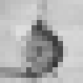
\includegraphics[width=0.1255\textwidth]{16pixel}}
\end{tabular}
\end{center}
\end{frame}

% New frame
\begin{frame}{Limitations with handcrafted prior models}
\structure{A priori information:} The image contains a rabbit.
\par\medskip
\visible<2->{
\structure{Designing $\RegFunc_{\param} \implies$ parametrise the notion of a rabbit}\par
Connected structure consisting of fused ellipsoids, two specific elongated structures near each other (ears), fibre-like texture (fur) with specific range of colours, \ldots then it is a rabbit!}
\par\bigskip
\centering
\visible<2->{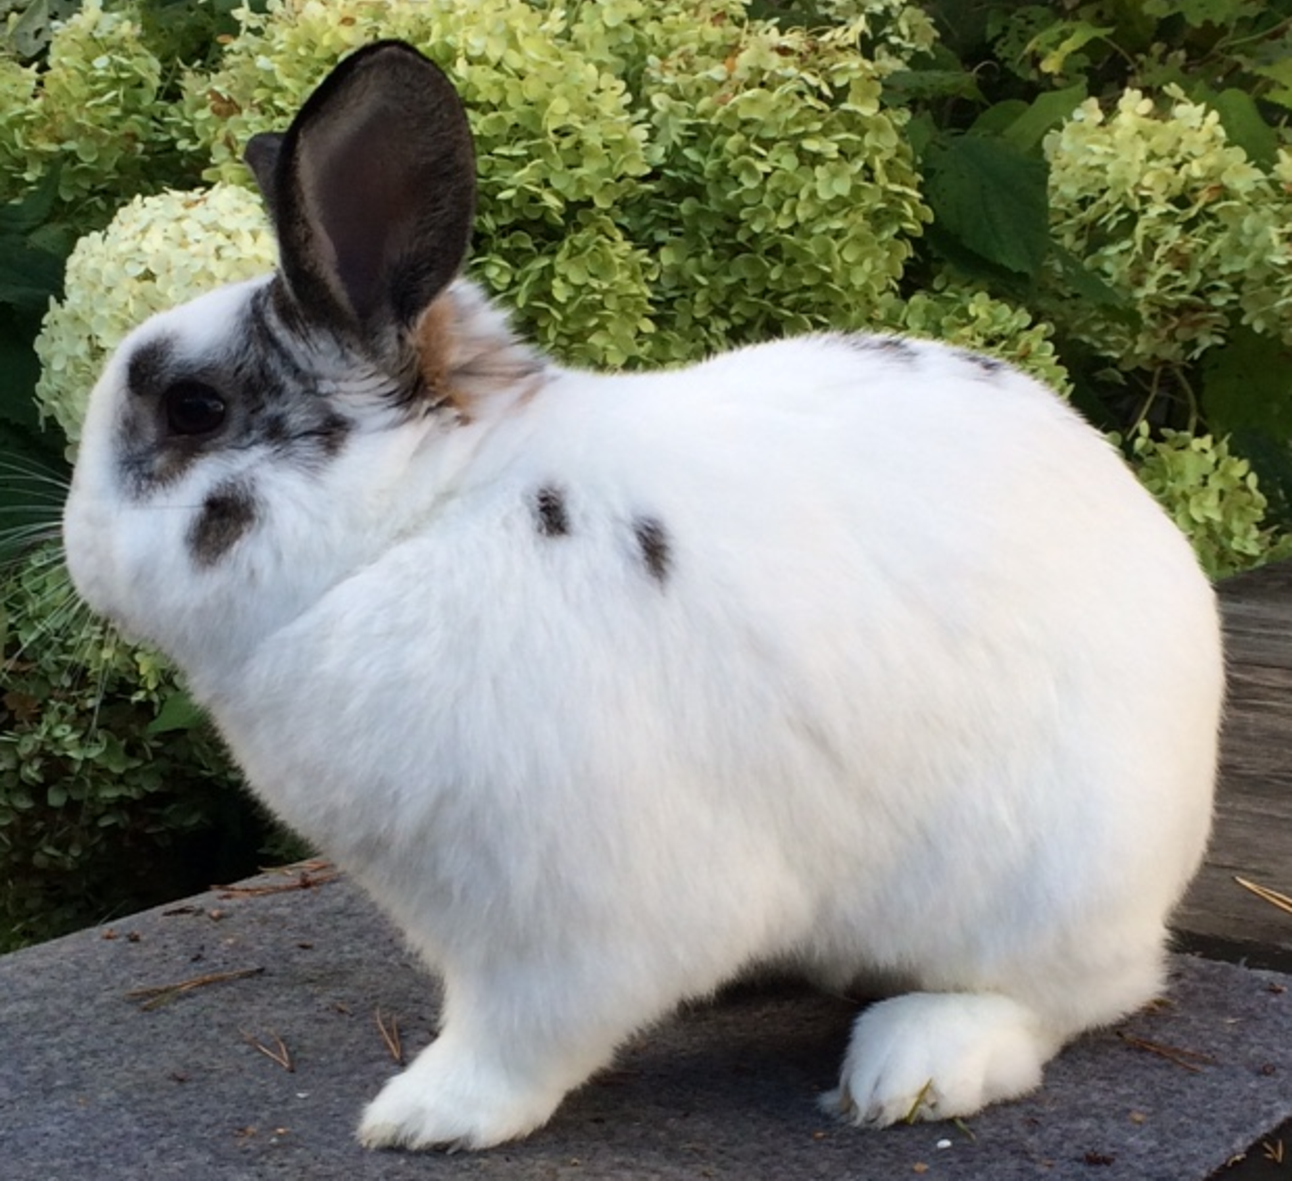
\includegraphics[height=0.6\textheight]{Onk_rabbit} \quad}
\visible<3>{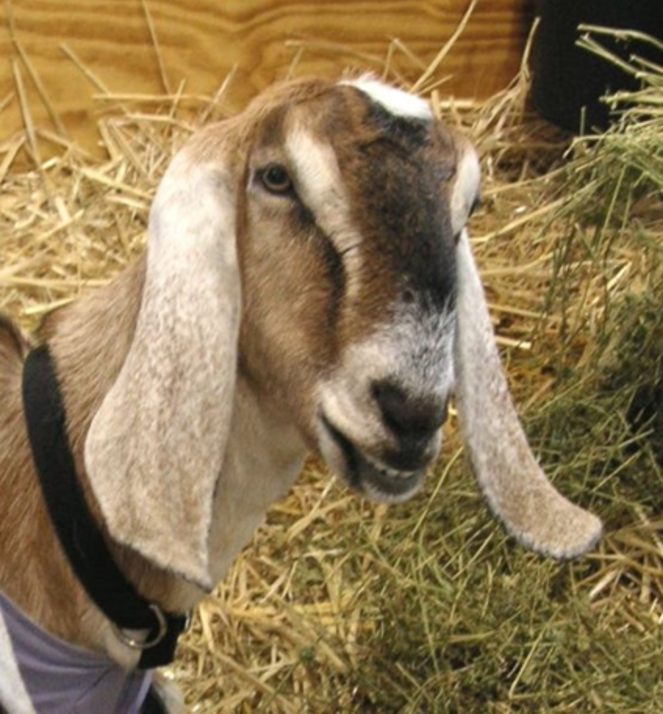
\includegraphics[height=0.6\textheight]{goat}}
\end{frame}


% New frame
\begin{frame}{Learned iterative reconstruction}{Approaches based on learning}
\par\medskip
\structure{Reconstruction methods based on learning}
\begin{itemize}
\item Learn prior and/or regularisation parameter in variational methods.
  \par $\implies$ Improves lack of flexibility in prior model.
  \par \qquad\, Does not improve upon computational feasibility.
  \par Se previous lecture (bi-level optimisation \& dictionary learning).
  %\cite{De-los-Reyes:2017aa,Xu:2012ab,Rusu:2017aa,Meinhardt:2017aa,Dokmanic:2016aa,Romano:2017aa}.
\visible<2->{
\item Learn how to iterate, i.e. learn an optimisation solver \cite{Gregor:2010aa,Oymak:2017aa,Giryes:2017aa}.
  \par $\implies$ Improves computational feasibility.
  \par \qquad\, Does not improve upon lack of flexibility in prior model.
%  \par \cite{Gregor:2010aa,Oymak:2017aa,Giryes:2017aa}
}
\visible<3->{
\item Learned reconstruction: Learn \alert<3>{both} the prior and how to iterate:
\begin{itemize}
\item \visible<4->{Fully learned reco. \cite{Argyrou:2012aa,Paschalis:2004aa,Zhu:2018aa}}
\item \visible<4->{Learned post-processing \cite{Kang:2017ab,Jin:2017aa}}
\item \visible<5>{\alert<5>{Learned iterative reconstruction}: Fourier inversion \cite{Yang:2016aa,Hammernik:2018aa}, 
  superesolution (small images) \cite{Putzky:2017aa},
  general (non-linear) inverse problem \cite{Adler:2017aa,Adler:2018aa}.
}
\end{itemize}
}
\end{itemize}
\end{frame}

% New frame
\begin{frame}{Learned iterative reconstruction}{Learned gradient descent}
\begin{columns}[T]
\begin{column}{0.5\textwidth}
\begin{algorithm}[H]
{\footnotesize
  \caption{Gradient descent}
  \begin{algorithmic}[1]
    \For{$i = 1, \dots$}
      \State $\signal_{i + 1} \gets 
        \signal_i - \alpha \bigl[\partial \ForwardOp(\signal_i)\bigr]^*\bigl(\ForwardOp(\signal_i) - \data \bigr)$
    \EndFor
  \end{algorithmic}
}  
\end{algorithm}
Solves variational problems with the following structure:
\[ \min_{\signal} \bigl\Vert \ForwardOp(\signal) - \data \bigr\Vert_\DataSpace^2 \]
\end{column}
\begin{column}{0.5\textwidth}
\visible<2>{%
\begin{algorithm}[H]
{\footnotesize
    \caption{Learned gradient descent}
    \begin{algorithmic}[1]
      \For{$i = 1, \dots, N$}
        \State $\signal_{i + 1} \gets \Lambda_{\param}\Bigl(\signal_i, 
           \bigl[\partial \ForwardOp(\signal_i)\bigr]^*\bigl(\ForwardOp(\signal_i) - \data\bigr)\Bigr)$
      \EndFor
      \State $\model{\param}(\data) \gets \signal_N$
  \end{algorithmic}
}
\end{algorithm}
\begin{itemize}
\item Finite number of iterates $N$.
\item
$\Lambda_{\param}$ given by a convolutional neural network (CNN), learn parameter $\param$ from training data in $\RecSpace \times \DataSpace$.
\end{itemize}
}
\end{column}
\end{columns}
\end{frame}

% New frame
\begin{frame}{Learned iterative reconstruction}{Learned primal-dual scheme}
\begin{overprint}
\onslide<1> %% Slide 1
\vskip-\baselineskip
\begin{columns}[T]
\begin{column}{0.5\textwidth}
\begin{algorithm}[H]
{\footnotesize 
    \caption{Non-linear PDHG}
    \begin{algorithmic}[1]
      \State \structure{Initialise:} $\sigma, \tau > 0$ s.t. $\sigma \tau \lVert \ForwardOp \rVert^2 < 1$, 
      \Statex $\zeta \in [0, 1]$ and $\primal_0 \in \RecSpace$, $\dual_0 \in \DataSpace$.
      \For{$i = 1, \dots$}
      \State $\dual_{i + 1} \gets \prox_{\sigma \OpF^*}\bigl(\dual_{i} + \sigma \ForwardOp(\bar{\primal}_{i}) \bigr)$ 
      \State $\primal_{i + 1} \gets \prox_{\tau \OpG}\bigl(\primal_{i} - \tau [ \partial \ForwardOp(\primal_{i})]^* (\dual_{i + 1}) \bigr)$
      \State $\bar{\primal}_{i + 1} \gets \primal_{i + 1} + \zeta (\primal_{i + 1} - \primal_{i})$
      \EndFor
    \end{algorithmic}
}  
  \end{algorithm}
Solves variational problems with the following structure:
\[  \min_{\primal \in \RecSpace} \Bigl[ \OpF\bigl( \ForwardOp(\primal)\bigr) + \OpG(\primal) \Bigr]  \]  
\end{column}
\begin{column}{0.5\textwidth}
\begin{algorithm}[H]
{\footnotesize 
    \caption{Learned PDHG}
      \begin{algorithmic}[1]
	\State \structure{Initialise:} $\primal_0 \in \RecSpace, \dual_0 \in \DataSpace$
	\For{$i = 1, \dots, N$}
	\State $\dual_{i+1} \gets
	\Gamma_{\param_{i+1}^d}\bigl(\dual_{i}, \ForwardOp(\primal_{i}), \data\bigr)$
	\State $\primal_{i+1} \gets 
	\Lambda_{\param_{i+1}^p}\bigl(\primal_{i}, [\partial\ForwardOp(\primal_{i})]^*(\dual_{i+1}) \bigr)$
	\EndFor
        \State $\model{\vparam}(\data) \gets \signal_N$
        \quad with $\vparam = (\param_1^d, \ldots, \param_N^p)$
      \end{algorithmic}
}
\end{algorithm}
\vskip-\baselineskip
\begin{itemize}
\item Unrolled primal-dual scheme inspired by the PDHG method. 
\item $\Gamma_{\param_i^d}$ and $\Lambda_{\param_i^p}$ given by CNNs, learn $\param_i^d$ and $\param_i^p$ from training data in $\RecSpace \times \DataSpace$ and \# iterates $N$.
\item Updates with memory 
  $\Longrightarrow$ learned primal dual method.
\end{itemize}
\end{column}
\end{columns}
\onslide<2> %% Slide 2
\begin{algorithm}[H]
{\footnotesize 
    \caption{Learned primal dual}
      \begin{algorithmic}[1]
	\State \structure{Initialise:} $\primal_0 \in \RecSpace \times \ldots \times \RecSpace$ ($N_p$ times),  $\dual_0 \in \DataSpace \times \ldots \times \DataSpace$ ($N_d$ times)
	\For{$i = 1, \dots, N$}
	\State $\dual_{i+1} \gets
	\Gamma_{\param_{i+1}^d}\bigl(\dual_{i}, \ForwardOp(\primal^{(2)}_{i}), \data\bigr)$
	\State $\primal_{i+1} \gets 
	\Lambda_{\param_{i+1}^p}\bigl(\primal_{i}, [\partial\ForwardOp(\primal^{(1)}_{i})]^*(\dual^{(1)}_{i+1}) \bigr)$
	\EndFor
        \State $\model{\vparam}(\data) \gets \signal^{(1)}_N$
        \quad with $\vparam = (\param_1^d, \param_1^p, \ldots, \param_N^d, \param_N^p)$
      \end{algorithmic}
}
\end{algorithm}
$\dual_i = ( \dual^{(1)}_i, \ldots, \dual^{(N_d)}_i )$

$\primal_i = ( \primal^{(1)}_i, \ldots, \primal^{(N_p)}_i )$

\onslide<3> %% Slide 3
\begin{itemize}
\item How to parametrise the learned operators $\Gamma_{\param^d}$ and $\Lambda_{\param^p}$?
\item Use recent advancements in deep learning and experience from variational regularisation:
  \begin{itemize}
  \item Translation invariance (convolutional networks) 
  \item Point-wise non-linearities
  \item Perturbations of the identity (residual networks)
  \end{itemize}
\item Structure for $\Gamma_{\param^d}$ (same for $\Lambda_{\param^p}$):
  \[ \Gamma_{\param} = \Id + W_{\param_3} \circ \rho_{2} \circ W_{\param_2} \circ \rho_{1} \circ W_{\param_1} \]
  $W$-operators of convolution type, $\rho$-operators pointwise non-linear (PReLU).
\item Example settings for 2D tomography:  
  \begin{itemize}
  \item In machine-learning lingo: `3 layer residual network with PReLU nonlinearities and $3 \times 3$ convolutions'
  \item Unroll with 10 `iterations' $\Longrightarrow$ 60 layers. 
  \item Deep learning network has `only' has $264\, 960$ parameters.
  \end{itemize}
\end{itemize}
\onslide<4> %% Slide 4
Network architecture
% \begin{center}
% 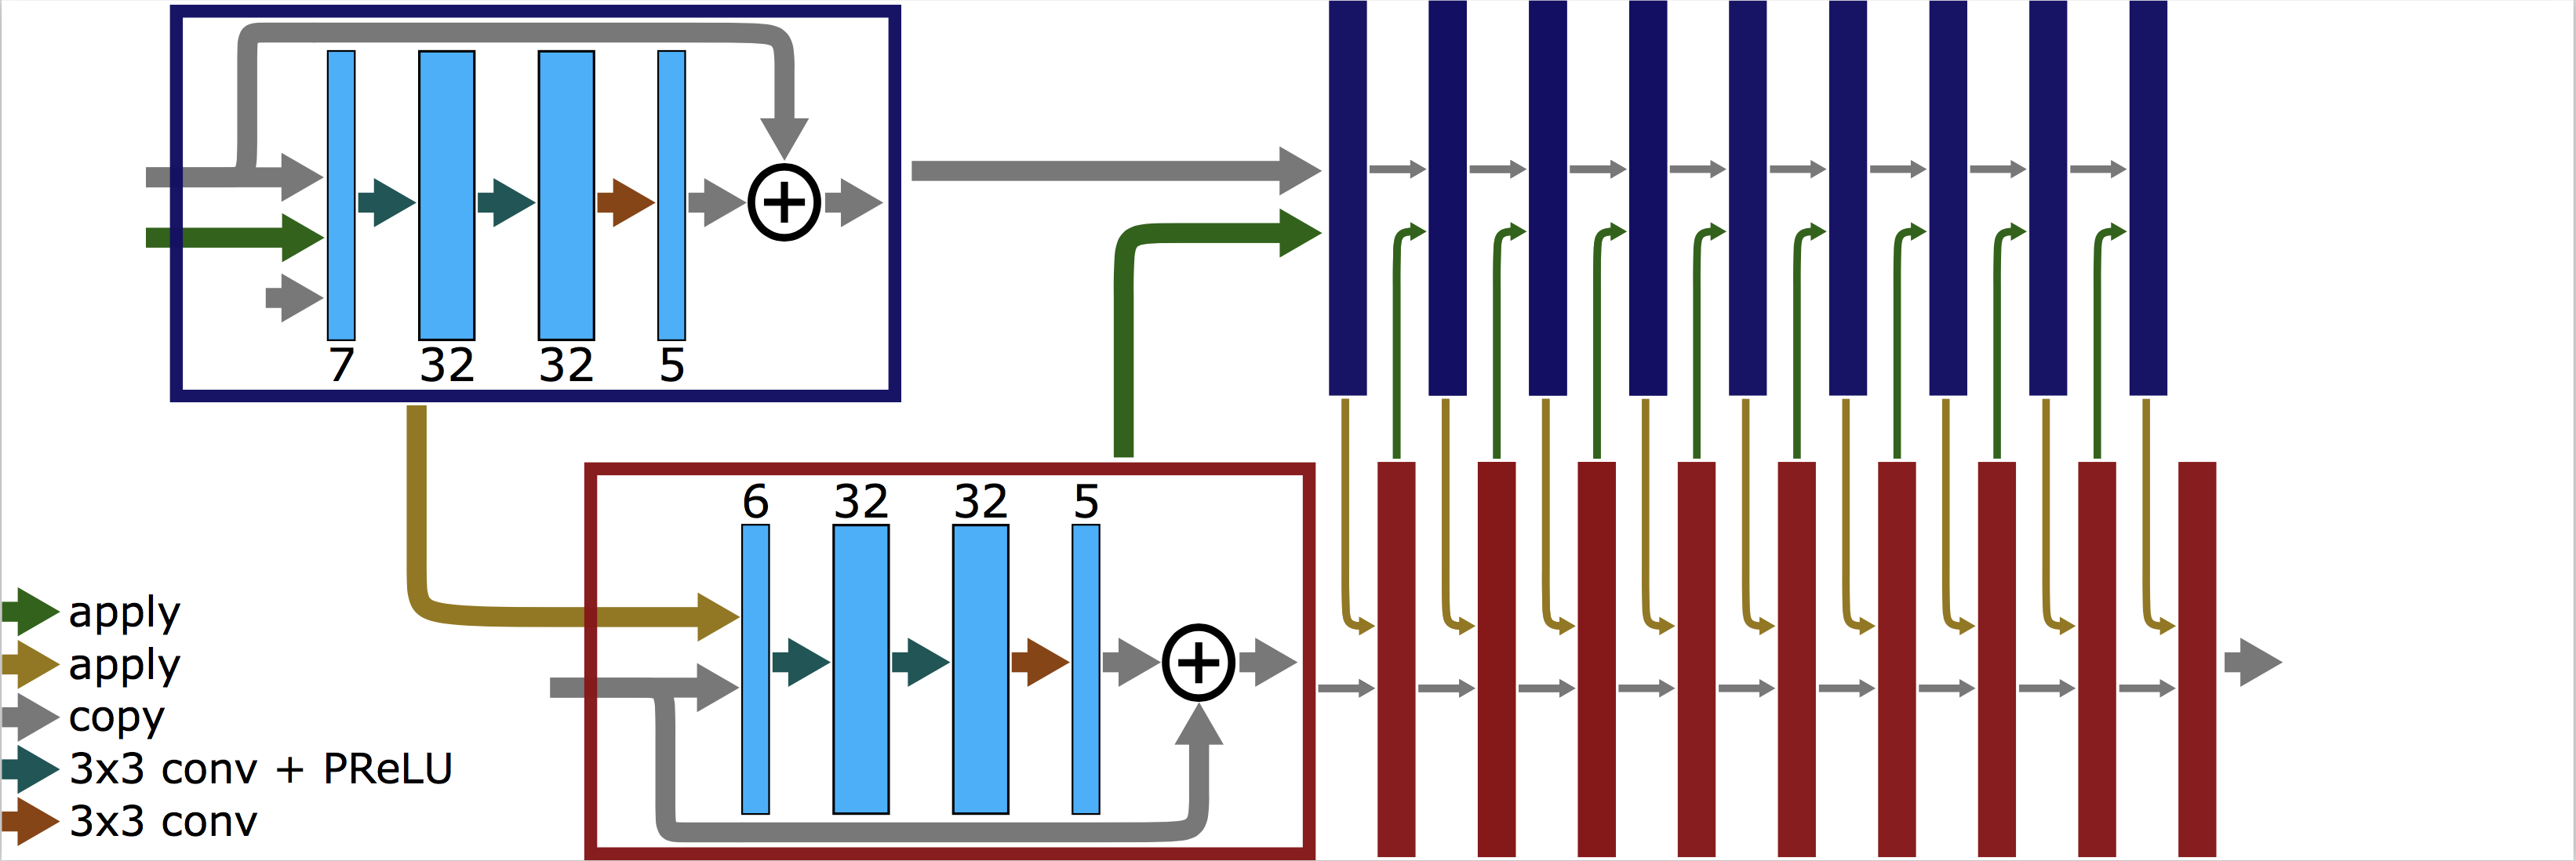
\includegraphics[width=0.95\linewidth]{primal_dual_network}
% \end{center}

\begin{tikzpicture}[overlay]
\node (img) at (current page.center) {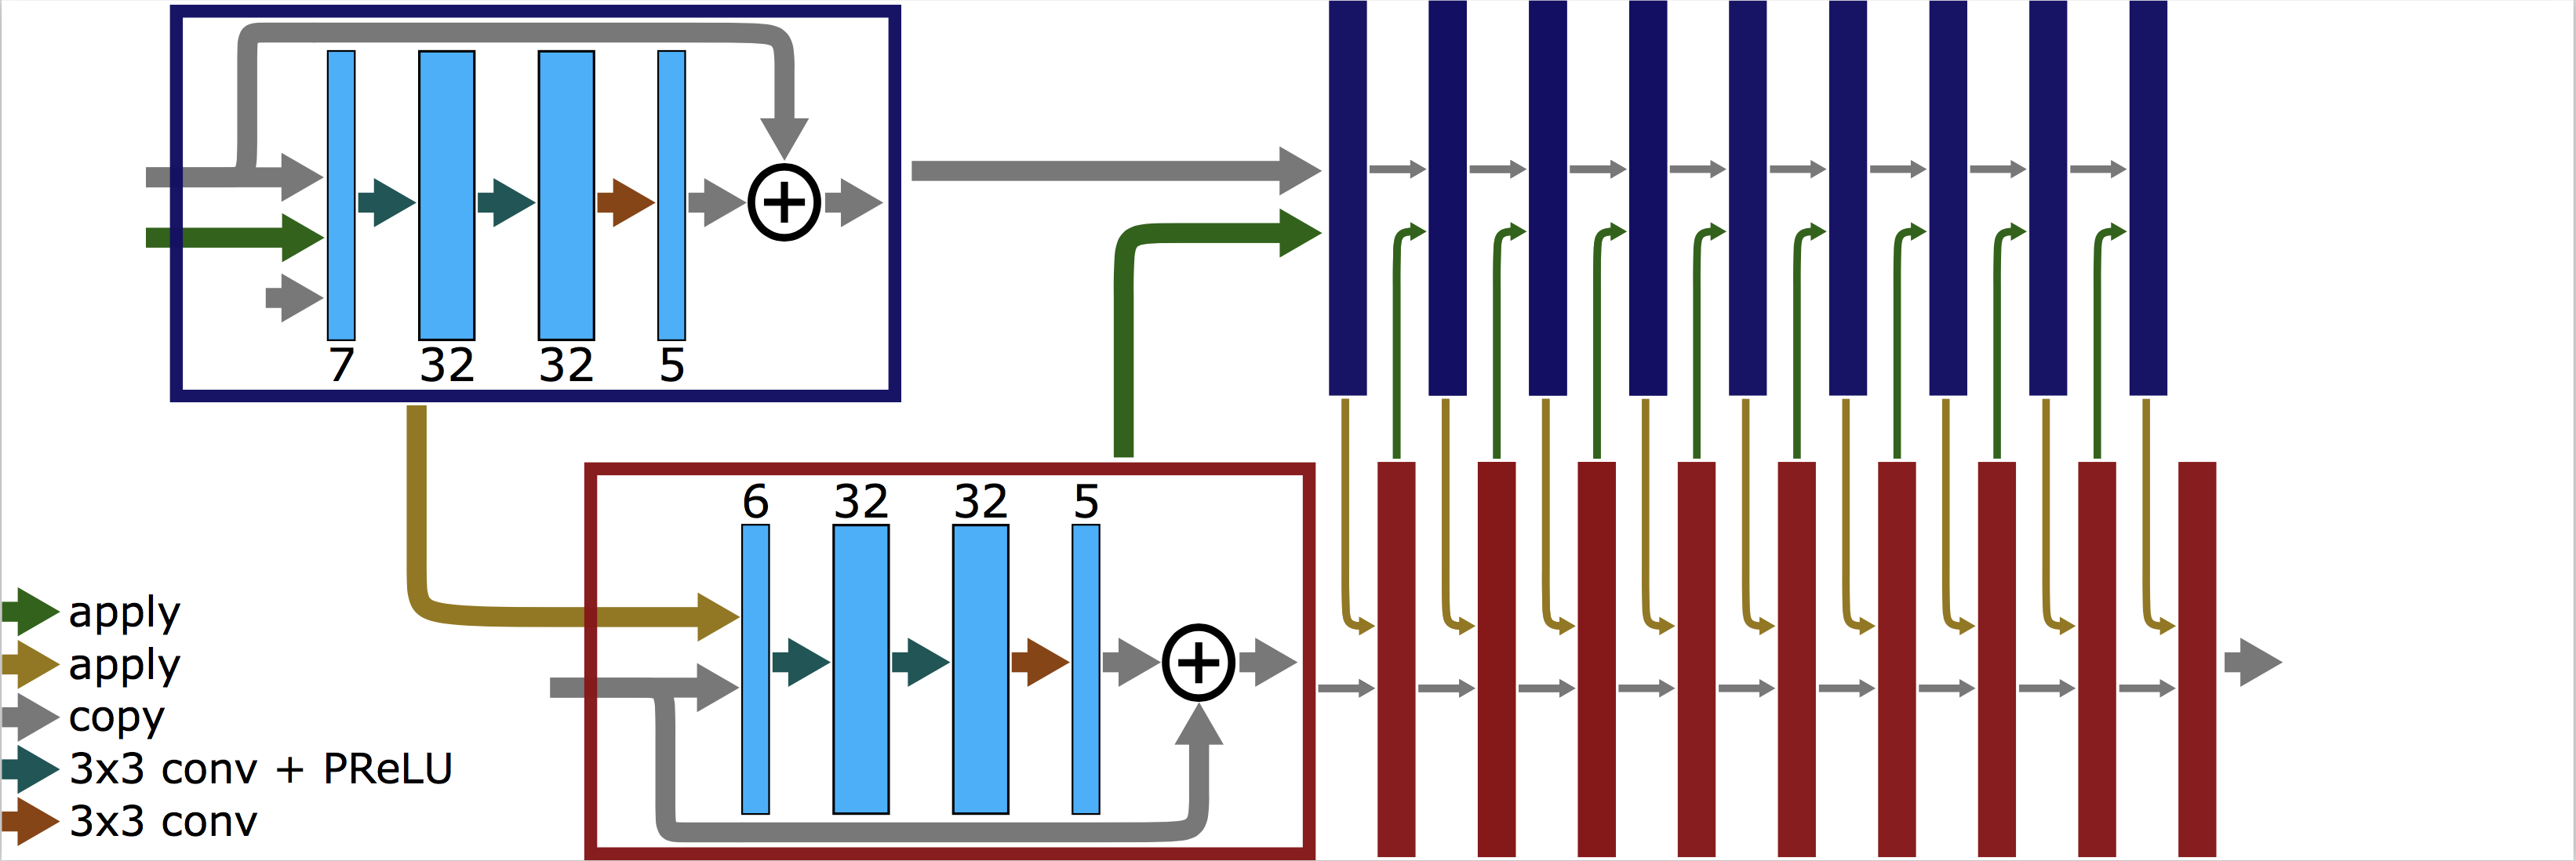
\includegraphics[width=0.95\linewidth]{primal_dual_network}};
% Data
\node [right,xshift=0.083\textwidth,yshift=-0.235\textheight] at (img.north west){\scriptsize{$\data$}};
% Initial primal
\node [right,xshift=0.03\textwidth,yshift=-0.19\textheight] at (img.north west){\scriptsize{$\primal_0$}};
\node [right,xshift=0.18\textwidth,yshift=-0.505\textheight] at (img.north west){\scriptsize{$\primal_0$}};
% Initial dual
\node [right,xshift=0.03\textwidth,yshift=-0.14\textheight] at (img.north west){\scriptsize{$\dual_0$}};
% Forward operator
\node [right,xshift=0.07\textwidth,yshift=-0.45\textheight] at (img.north west){\scriptsize{$\ForwardOp$}};
% Adjoint of derivative of forward operator
\node [right,xshift=0.07\textwidth,yshift=-0.495\textheight] at (img.north west){\scriptsize{$[ \partial\!\ForwardOp]^*$}};
% Reconstruction operator
\node [right,xshift=0.37\textwidth,yshift=-0.165\textheight] at (img.center){\scriptsize{$\model{\param}(\data)$}};
% Textbox
\node [right,text width=0.9\textwidth,align=left,yshift=-0.1\textheight] at (img.south west)%
  {Dual iterates are in blue boxes, primal iterates are in red boxes. The initial guesses enter from the left, while the data is supplied to the dual iterates.};
\end{tikzpicture} 
\end{overprint}
\end{frame}



\begin{frame}{2D tomography of Shepp-Logan}
\framesubtitle{Set-up}
\structure{Inverse problem:} Reconstruct 2D image from sinogram (tomographic data)
\[
\data = \ForwardOp(\signal) + \datanoise
\]
\vskip-0.5\baselineskip
\begin{itemize}
\item Forward operator:  2D ray transform 
\item Geometry: Parallel beam, 30 directions, 182 lines/directions
\item Noise: $5\%$ additive Gaussian
\item Image: $128 \times 128$ pixel
\item Training data: 50\,000 pairs (ellipses, sinogram)
\end{itemize}

\structure{Reconstruction methods:}
\begin{itemize}
\item Filtered backprojection (FBP): Standard clinical protocol \cite{Natterer:2001aa}.
\item Total variation (TV) \cite{Sidky:2012aa}.
\item FBP + U-Net denoising: Won 2016 low-dose CT challenge \cite{Kang:2017aa}.
\item Learned Primal-Dual in Shearlets.
\item Learned Primal-Dual \cite{Adler:2018aa}.
\item Conditional expectation (by MCMC).
\end{itemize}
\end{frame}

\begin{frame}[plain]
\setlength{\lineskip}{0pt}%<======== here
\begin{columns}[t]
\begin{column}{0.5\textwidth}
\begin{center}
\begin{minipage}{\textwidth}
\centering
Phantom\\ \rule{0pt}{2pt}
\end{minipage}\\
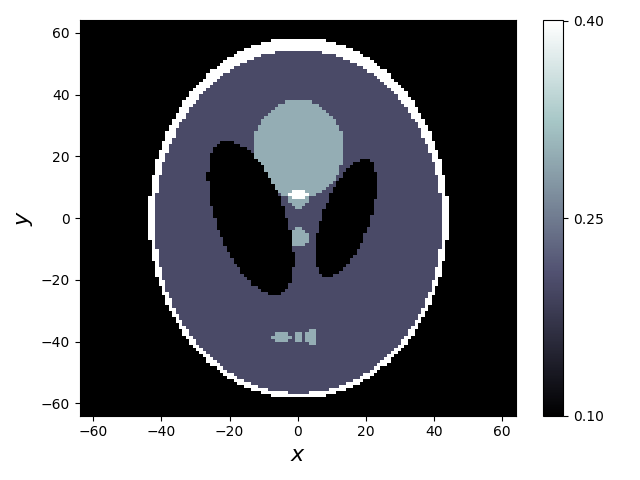
\includegraphics[width=\textwidth, trim={23mm 16mm 27mm 6mm}, clip]{shepp_logan_phantom_windowed} \\
\end{center}
\end{column}
\begin{column}{0.5\textwidth}
\begin{center}
\only<1>{
\begin{minipage}{\textwidth}
\centering
Training Phantom\\ \rule{0pt}{0pt}
\end{minipage}\\
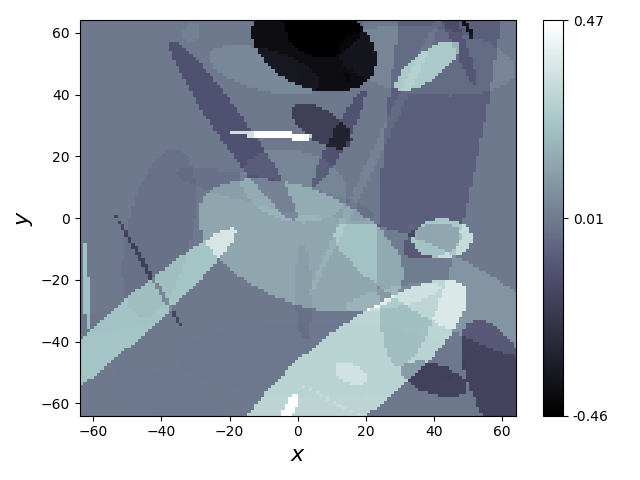
\includegraphics[width=\linewidth, trim={23mm 16mm 27mm 6mm}, clip]{ellipse_phantom} \\
}
\only<2>{
\begin{minipage}{\textwidth}
\centering
FBP\\ \rule{0pt}{0pt}
\end{minipage}\\
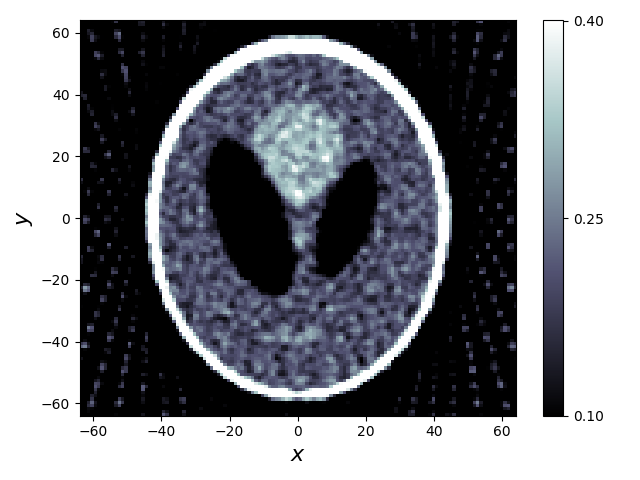
\includegraphics[width=\textwidth, trim={23mm 16mm 27mm 6mm}, clip]{shepp_logan_fbp_windowed} \\
}
\only<3>{
\begin{minipage}{\textwidth}
\centering
TV\\ \rule{0pt}{0pt}
\end{minipage}\\
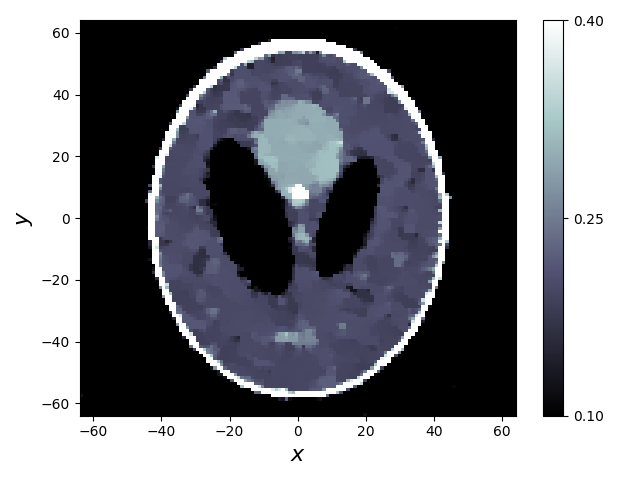
\includegraphics[width=\textwidth, trim={23mm 16mm 27mm 6mm}, clip]{shepp_logan_tv_windowed} \\
}
\only<4>{
\begin{minipage}{\textwidth}
\centering
FBP + Learned post-processing\\ \rule{0pt}{0pt}
\end{minipage}\\
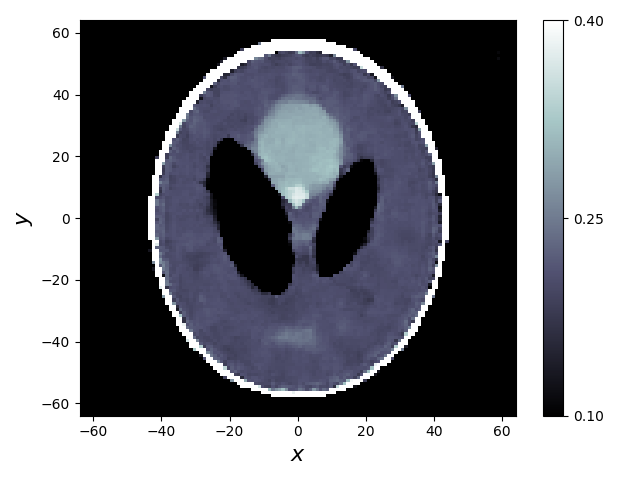
\includegraphics[width=\textwidth, trim={23mm 16mm 27mm 6mm}, clip]{shepp_logan_result_u_net} \\
}
\only<5>{
\begin{minipage}{\textwidth}
\centering
Learned Primal-Dual in Shearlets\\ \rule{0pt}{0pt}
\end{minipage}\\
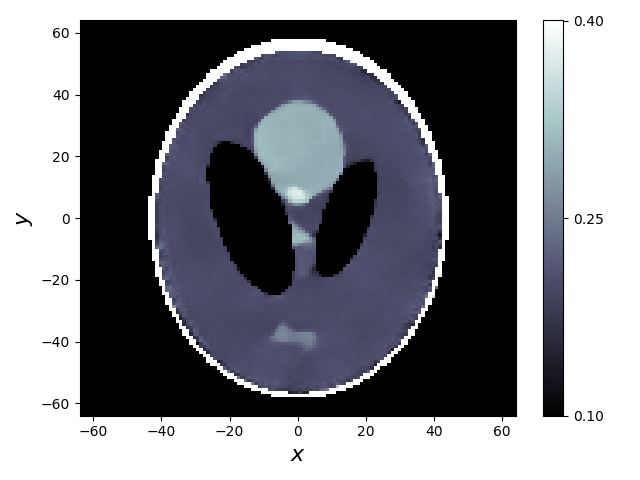
\includegraphics[width=\textwidth, trim={23mm 16mm 27mm 6mm}, clip]{primal_dual_ellipses_result_shearlets} \\
}
\only<6>{
\begin{minipage}{\textwidth}
\centering
Learned Primal-Dual\\ \rule{0pt}{0pt}
\end{minipage}\\
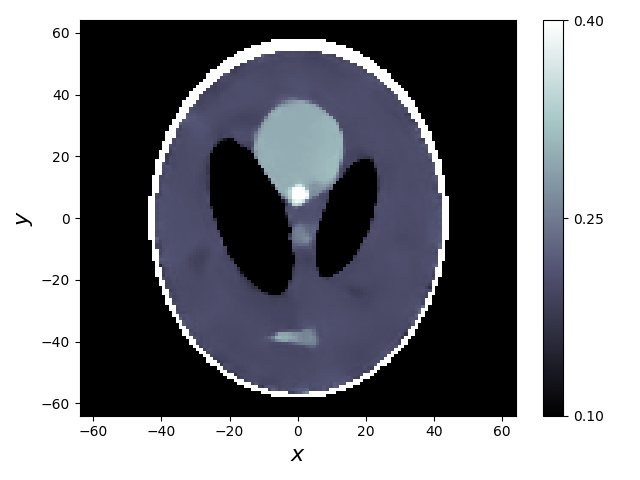
\includegraphics[width=\textwidth, trim={23mm 16mm 27mm 6mm}, clip]{primal_dual_ellipses_result} \\
}
\only<7>{
\begin{minipage}{\textwidth}
\centering
Conditional expectation\\ \rule{0pt}{0pt}
\end{minipage}\\
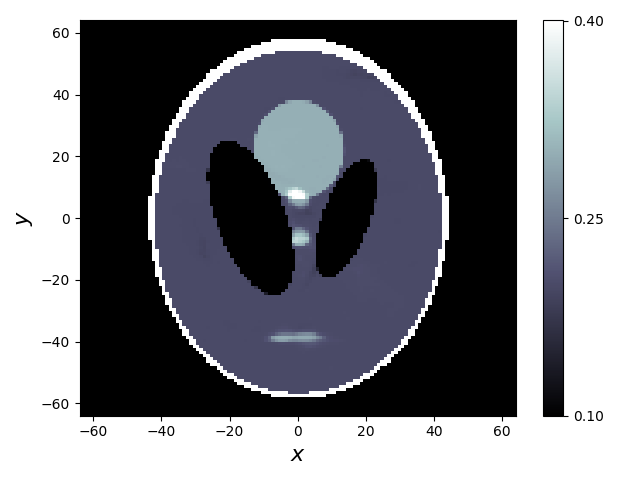
\includegraphics[width=\textwidth, trim={23mm 16mm 27mm 6mm}, clip]{shepp_logan_conditional_expectation} \\
}
\end{center}
\end{column}
\end{columns}
\end{frame}

\begin{frame}{2D tomography of Shepp-Logan}{Quantitative comparison}
{\small
\begin{tabular}{ l r r r}
\toprule
Method & PSNR (dB) & SSIM & Parameters\\
\midrule
FBP  & 19.75 & 0.597 & 1 \\
TV & 28.06 & 0.928 & 1 \\
Learned U-Net & 29.20 & 0.943 & $10^7$\\
Learned Primal-Dual & 38.28 & 0.988 & $2.4 \cdot 10^5$\\
Conditional expectation & 45.46 & 0.993 & $0$\\
\bottomrule
\end{tabular}
\par\bigskip
SSIM = structural similarity index, ($1$ perfect match).
\par\bigskip
\begin{itemize}
\item Very large quantitative improvement
\item Noticeable visual improvement
\item Very competitive speed
\item We are remarkably close to the theoretical optimum!!
\end{itemize}
}
\end{frame}

% New frame
\begin{frame}{Tomography of anthropomorphic phantom}{Set-up}
\structure{Inverse problem:} Recover attenuation coefficient from tomographic data (sinogram).
\begin{itemize}
\item Simulator: Radiative transport equation + noise.
\item Noise: Poisson noise with $10^4$ incident photons/pixel (\alert{low dose CT}).
\item Digitisation of data: Fan beam with 1000 lines/angle, 1000 angles.
\item Digitisation of model parameter: $512 \times 512$ pixel 2D image of attenuation coefficient.
\item \alert{Deep learning training data}: 2\,000 pairs of $(\text{`image'},\text{`noisy data'})$ from \alert{9~patients}. 
\end{itemize}

\structure{Reconstruction methods:}
\begin{itemize}
\item Filtered backprojection (FBP): Standard clinical protocol \cite{Natterer:2001aa}.
\item Total variation (TV) \cite{Sidky:2012aa}.
\item FBP + U-Net denoising: Won 2016 low-dose CT challenge \cite{Kang:2017aa}.
\item Learned Primal-Dual \cite{Adler:2018aa}.
\end{itemize}
\end{frame}

% New frame
\begin{frame}[plain]
\begin{columns}[b]
\begin{column}{0.5\textwidth}
\begin{center}
\begin{tikzpicture}[
      overlay,
      remember picture,
      spy using outlines={%
        circle,
        red,
        magnification=5,
        size=1.5cm,
        connect spies
        }
  ]
  \node {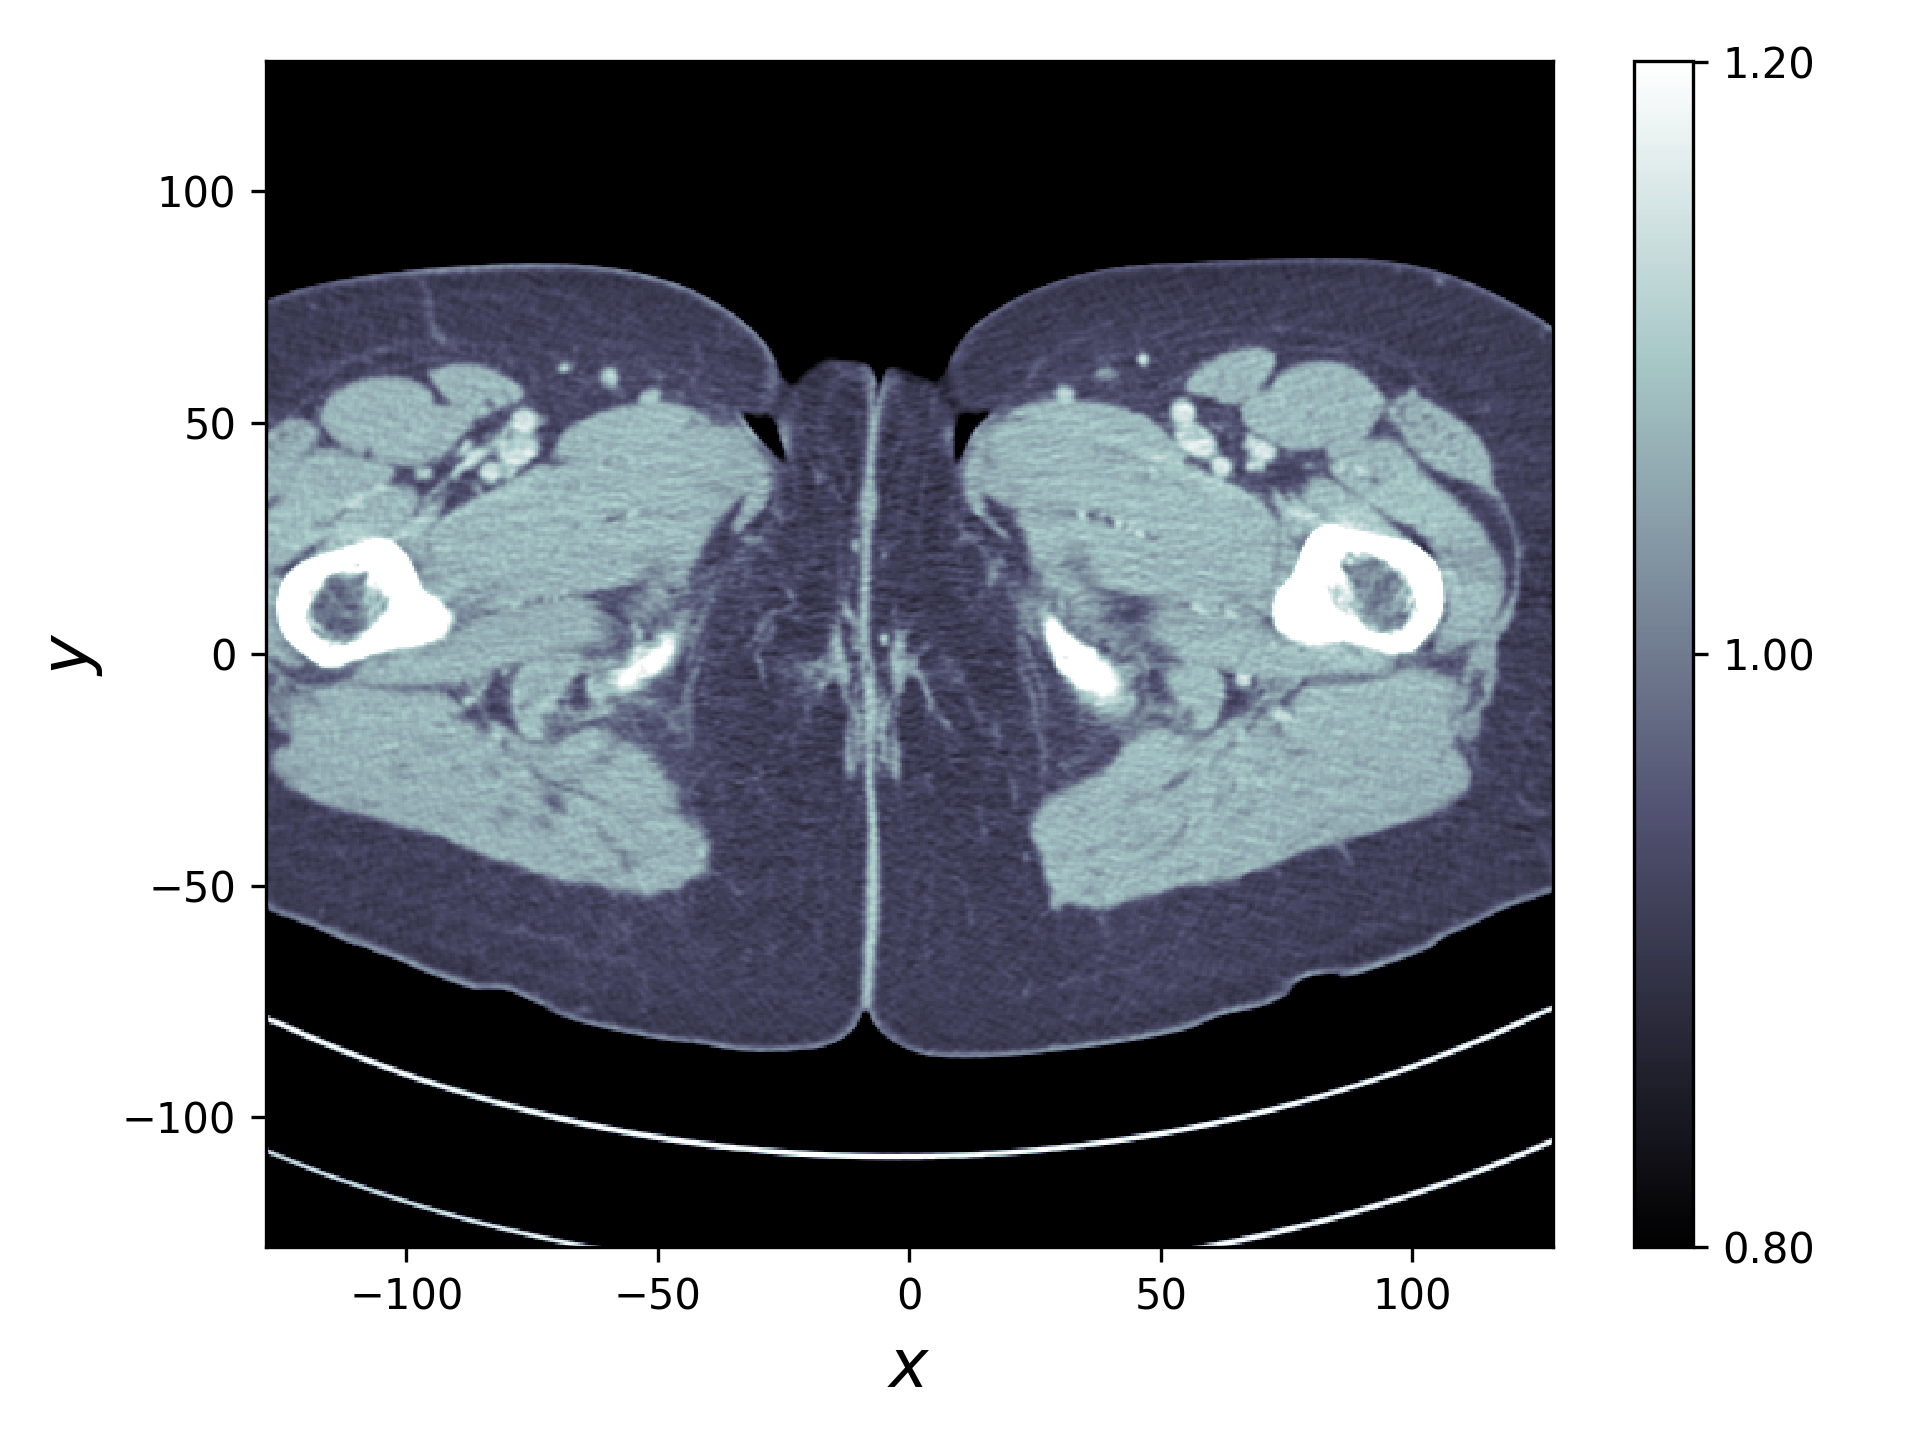
\includegraphics[width=\linewidth, trim={22.5mm 16mm 27mm 6mm}, clip]{mayo_phantom}};
  \node[text centered,xshift=0.6\textwidth,yshift=0.2\textheight] at (current page.south west) {\captionfix{Ground truth.}};
  \only<2->{
  \spy on (-1.7,0.8) in node [left] at (-0.5,3);
  \spy on (2,1.2) in node [left] at (2.4,3);}
\end{tikzpicture}
\end{center}
\end{column}
\begin{column}{0.5\textwidth}
\begin{overprint}
%and FBP
\onslide<3>
\begin{center}
\begin{tikzpicture}[
      overlay,
      remember picture,
      spy using outlines={%
        circle,
        red,
        magnification=5,
        size=1.5cm,
        connect spies
        }
  ]
  \node {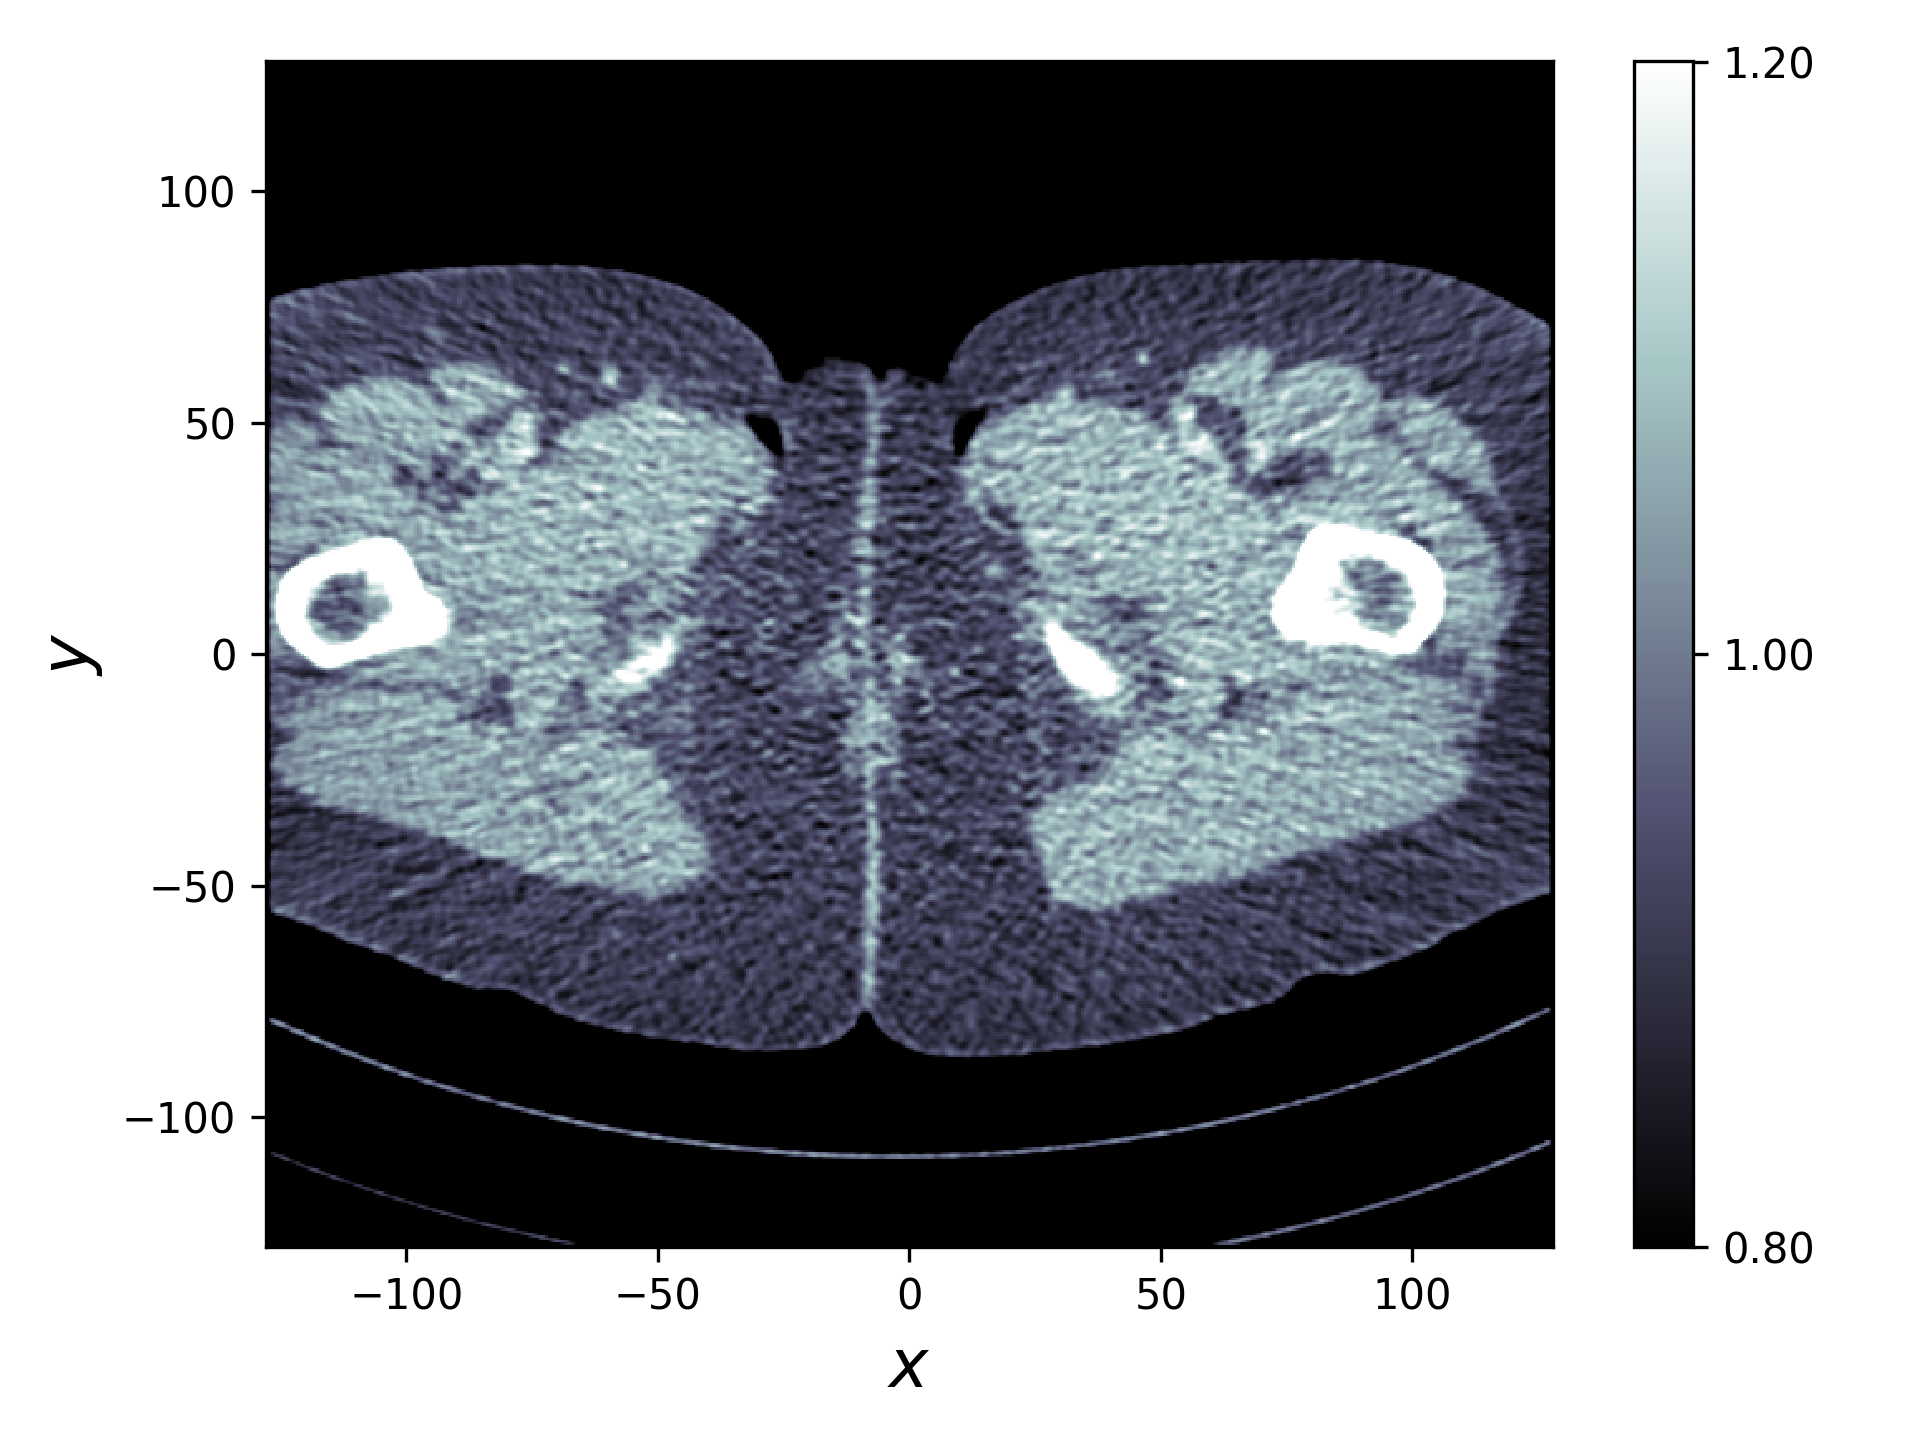
\includegraphics[width=\linewidth, trim={22.5mm 16mm 27mm 6mm}, clip]{mayo_fbp}};
  \node[text centered,xshift=1.7\textwidth,yshift=0.2\textheight] at (current page.south west) {\captionfix{FBP reconstruction.}};
  \spy on (-1.7,0.8) in node [left] at (-0.5,3);
  \spy on (2,1.2) in node [left] at (2.4,3);
\end{tikzpicture}
\end{center}
% TV
\onslide<4>
\begin{center}
\begin{tikzpicture}[
      overlay,
      remember picture,
      spy using outlines={%
        circle,
        red,
        magnification=5,
        size=1.5cm,
        connect spies
        }
  ]
  \node {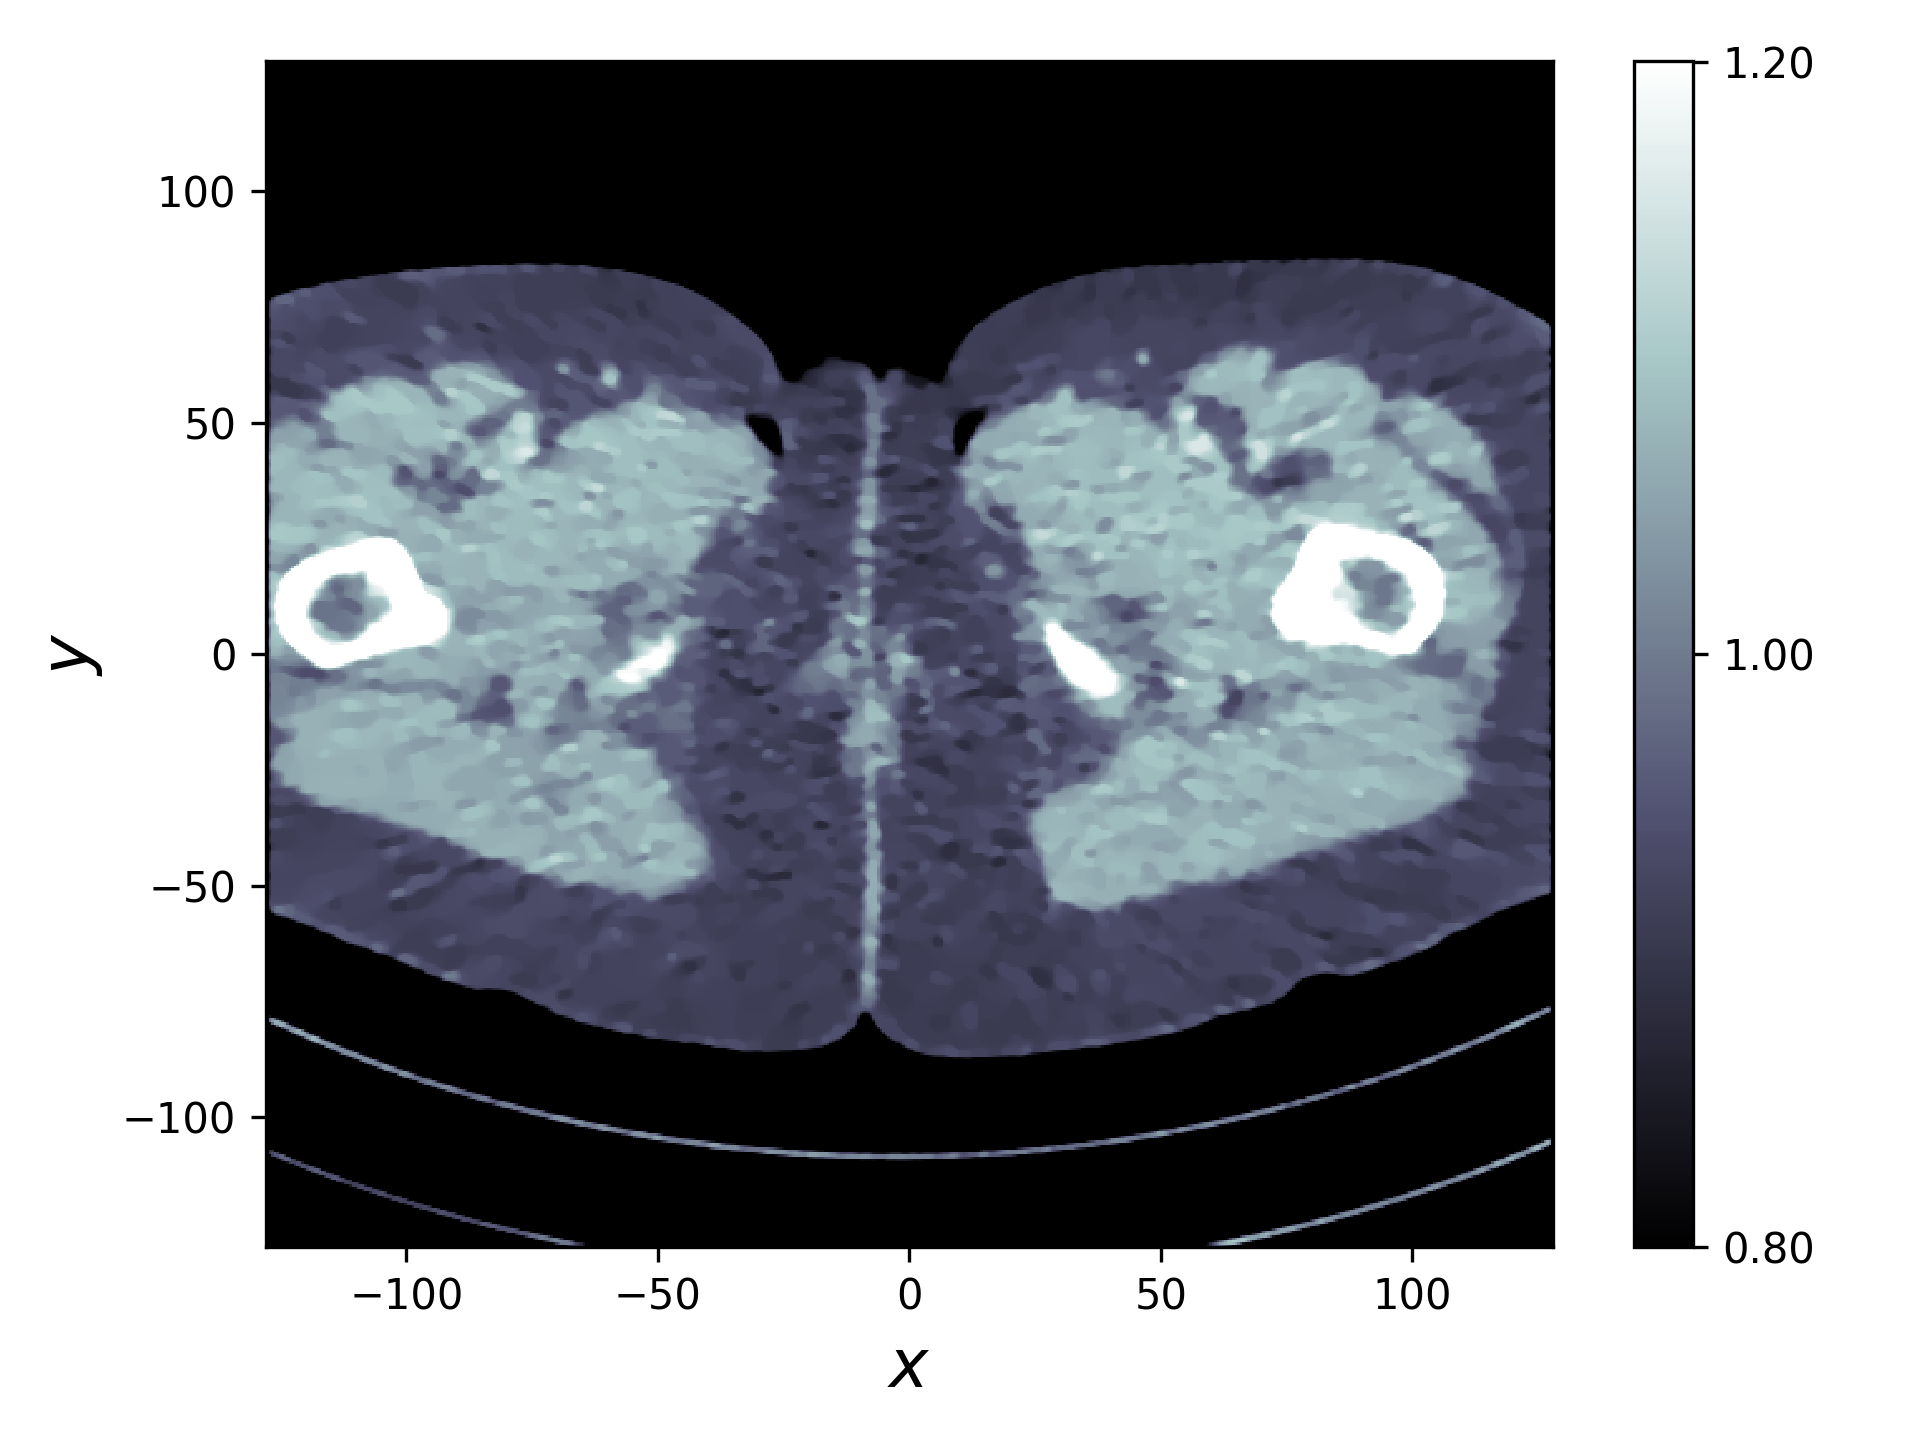
\includegraphics[width=\linewidth, trim={22.5mm 16mm 27mm 6mm}, clip]{mayo_tv}};
  \node[text centered,xshift=1.7\textwidth,yshift=0.2\textheight] at (current page.south west) {\captionfix{TV reconstruction.}};
  \spy on (-1.7,0.8) in node [left] at (-0.5,3);
  \spy on (2,1.2) in node [left] at (2.4,3);
\end{tikzpicture}
\end{center}
% FBP + Unet
\onslide<5>
\begin{center}
\begin{tikzpicture}[
      overlay,
      remember picture,
      spy using outlines={%
        circle,
        red,
        magnification=5,
        size=1.5cm,
        connect spies
        }
  ]
  \node {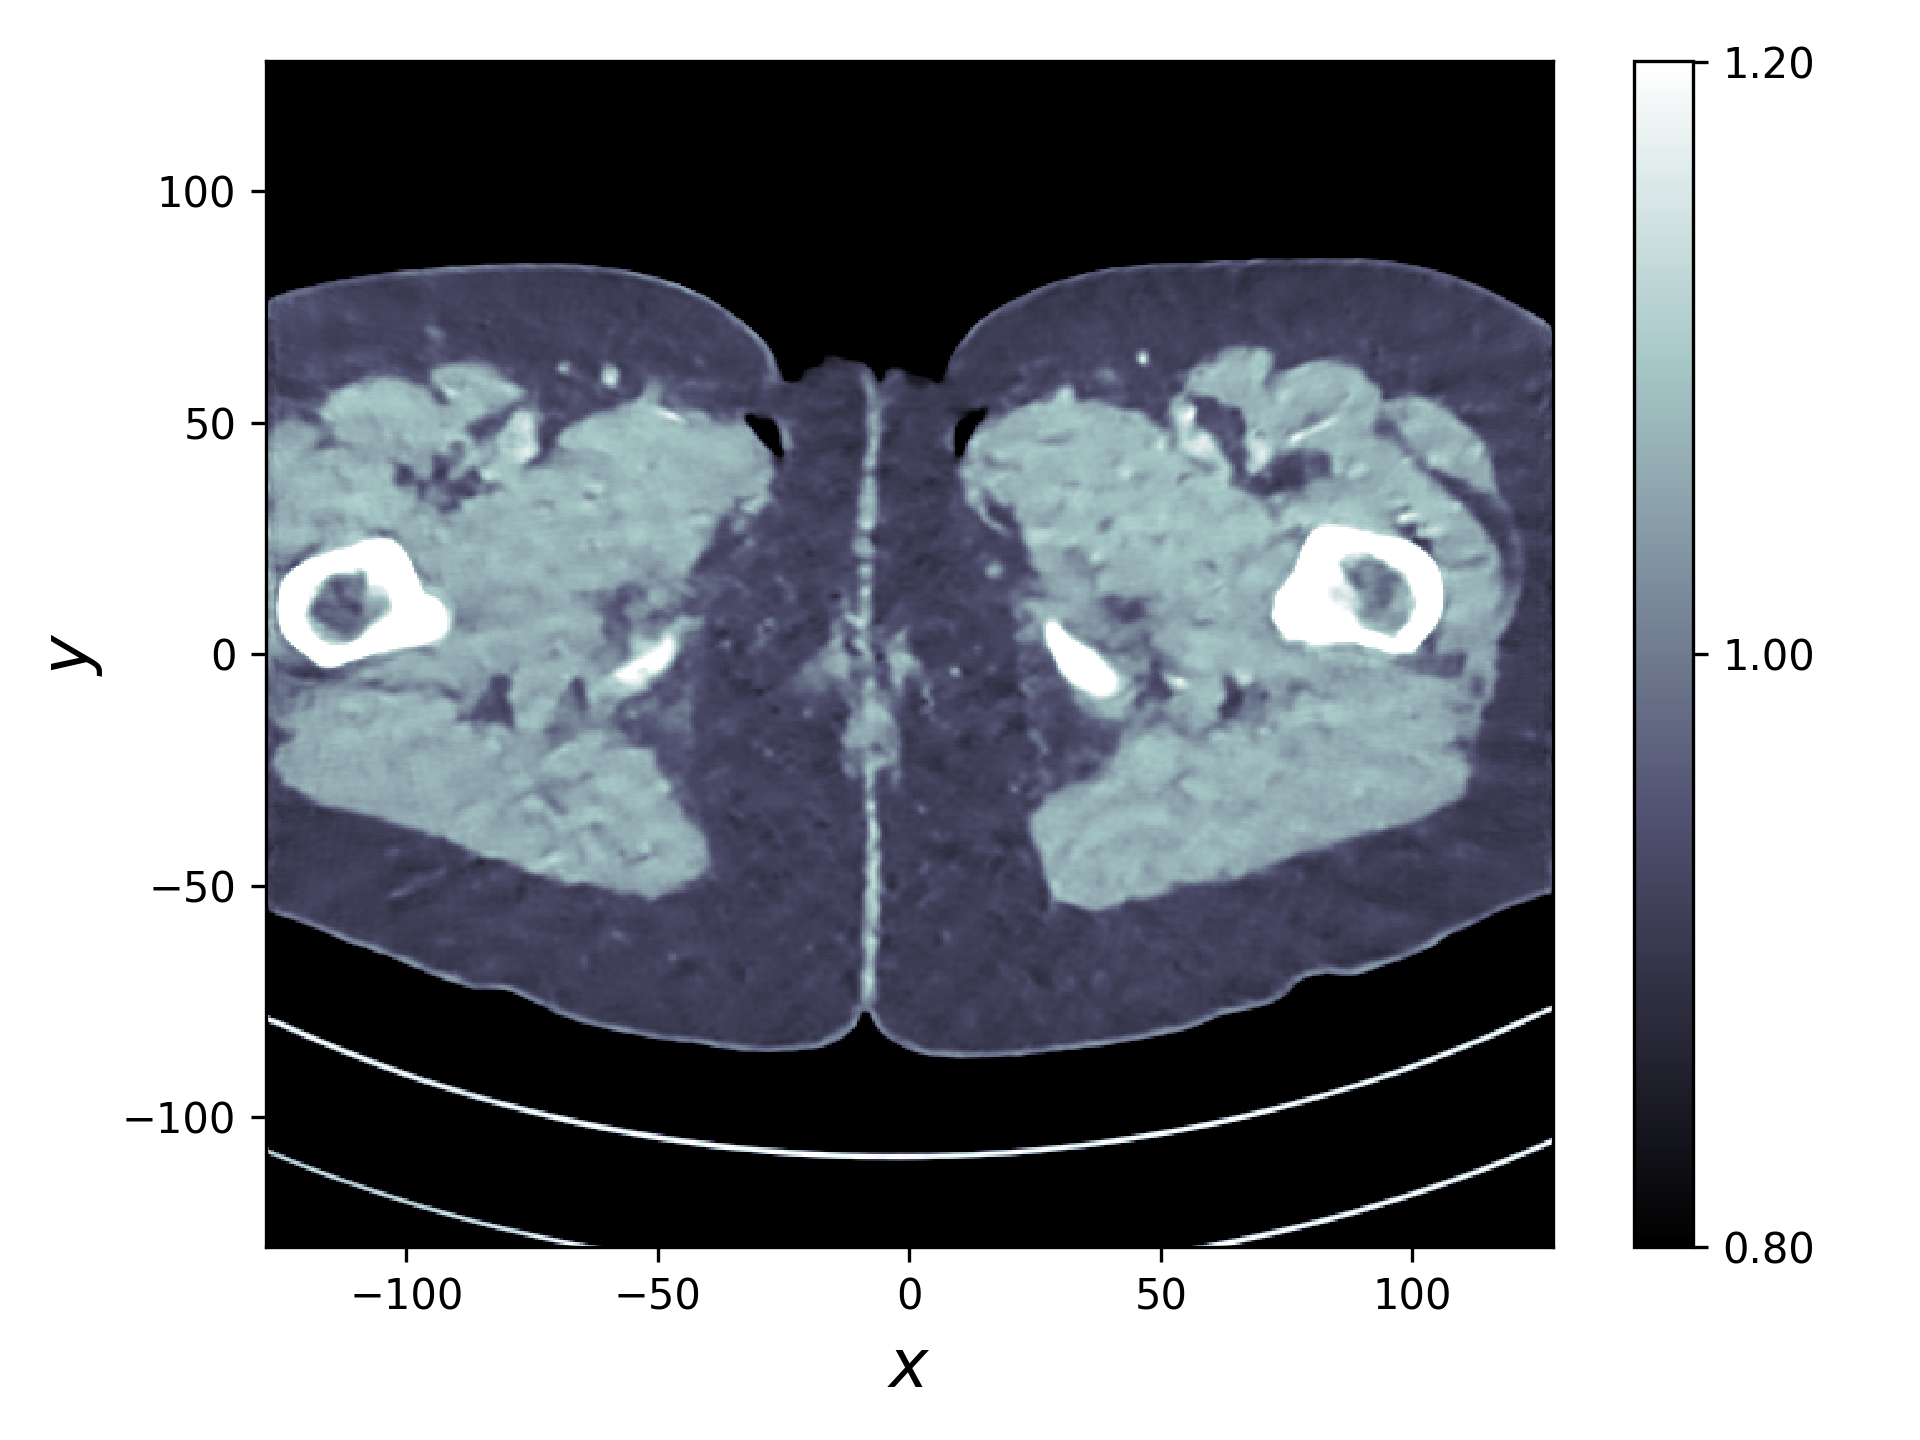
\includegraphics[width=\linewidth, trim={22.5mm 16mm 27mm 6mm}, clip]{mayo_unet}};
  \node[text centered,xshift=1.7\textwidth,yshift=0.2\textheight] at (current page.south west) {\captionfix{FBP + U-Net denoising.}};
  \spy on (-1.7,0.8) in node [left] at (-0.5,3);
  \spy on (2,1.2) in node [left] at (2.4,3);
\end{tikzpicture}
\end{center}
% Learned primal-dual
\onslide<6>
\begin{center}
\begin{tikzpicture}[
      overlay,
      remember picture,
      spy using outlines={%
        circle,
        red,
        magnification=5,
        size=1.5cm,
        connect spies
        }
  ]
  \node {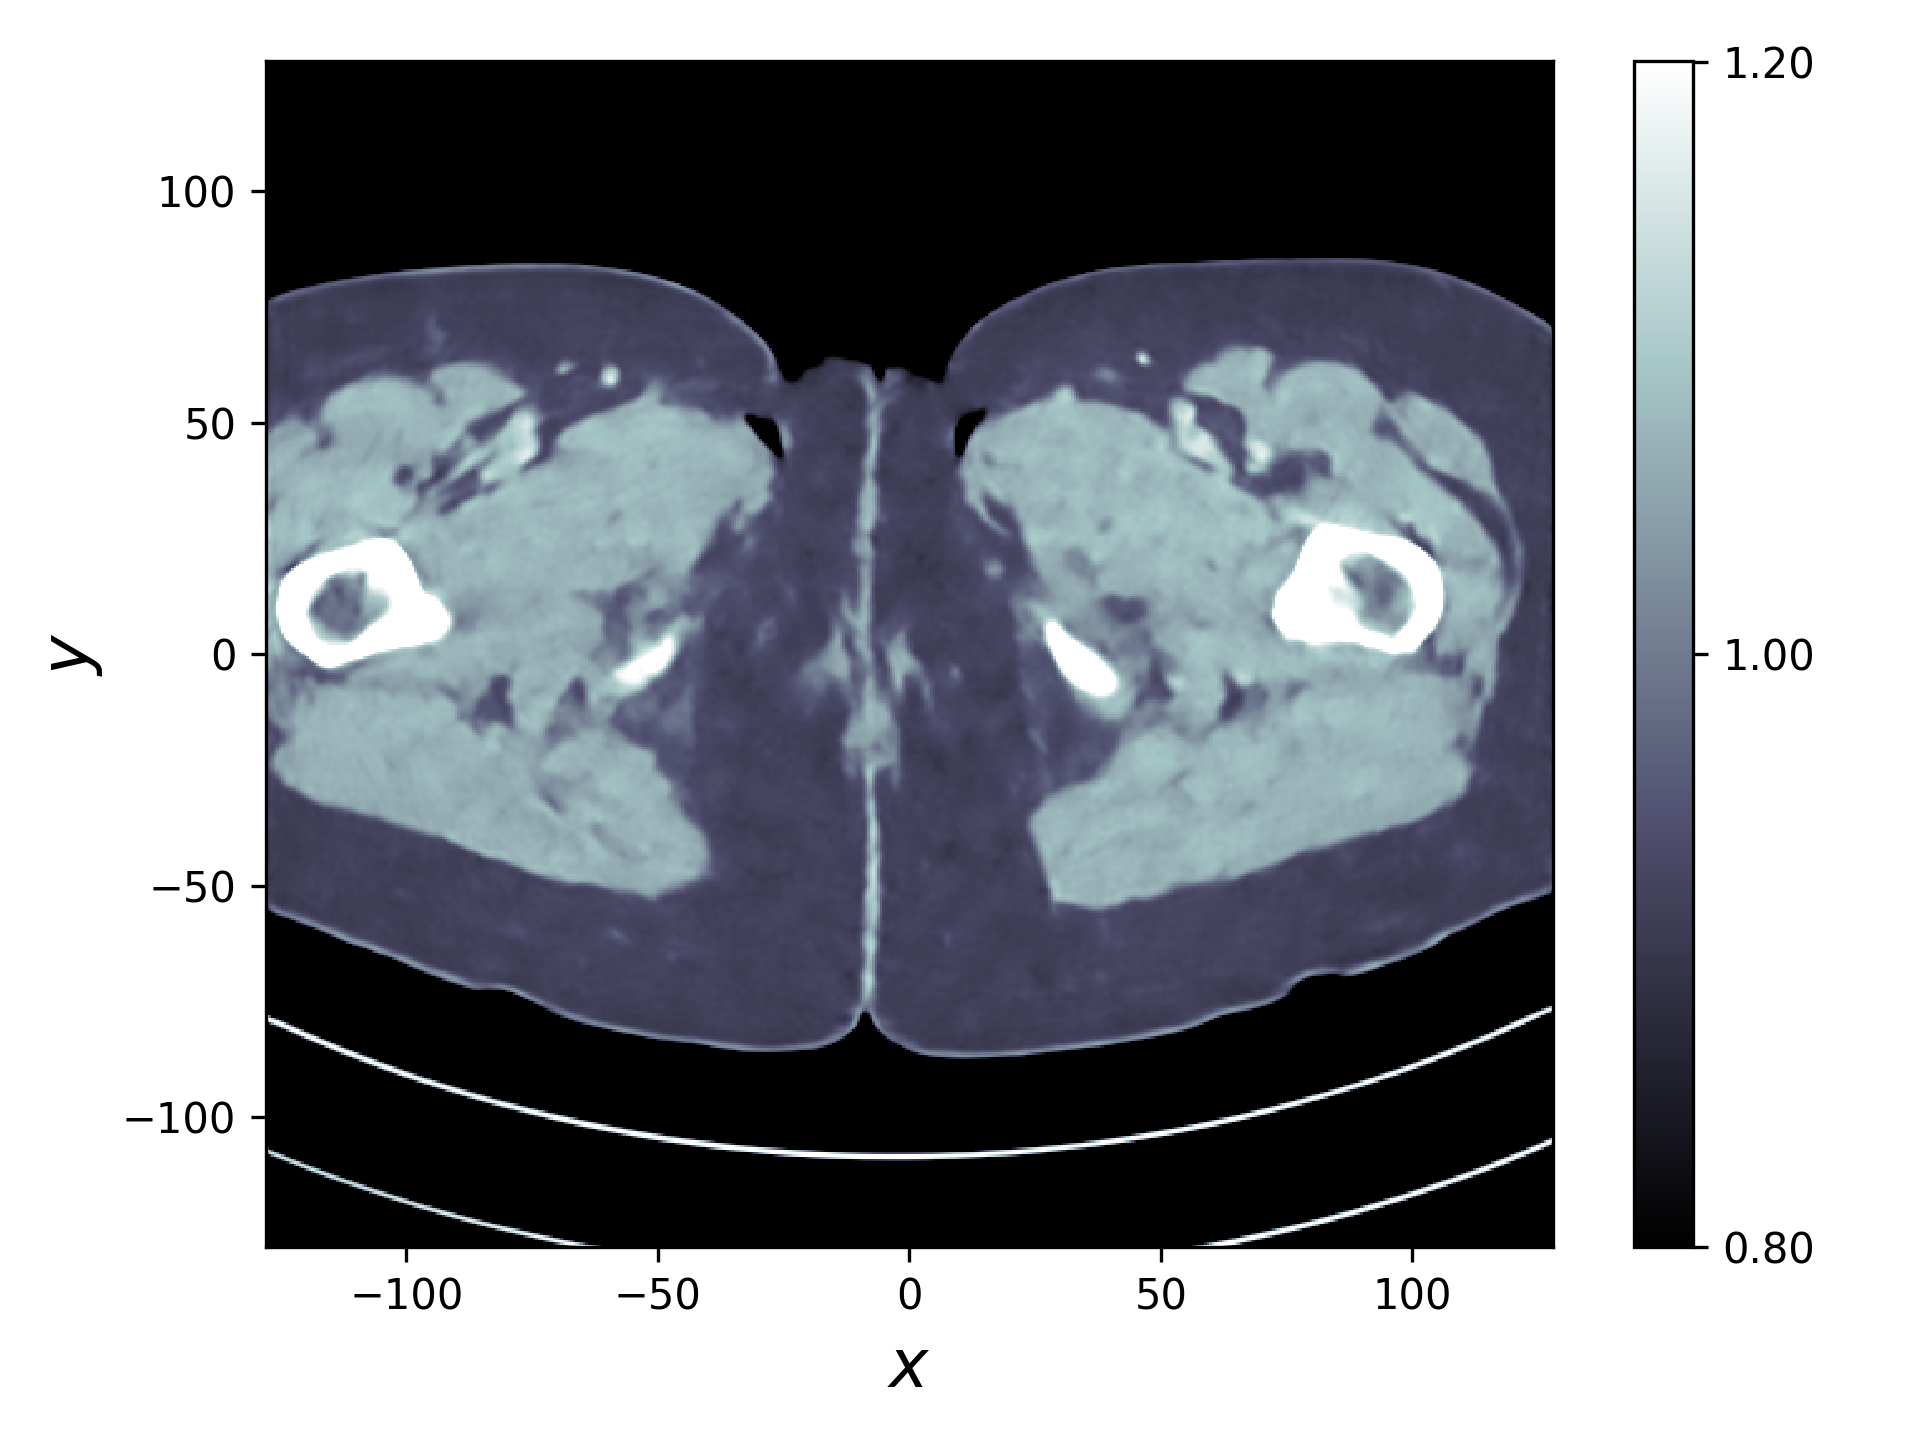
\includegraphics[width=\linewidth, trim={22.5mm 16mm 27mm 6mm}, clip]{mayo_learned_pd_log}};
  \node[text centered,xshift=1.7\textwidth,yshift=0.2\textheight] at (current page.south west) {\captionfix{Learned Primal-Dual.}};
  \spy on (-1.7,0.8) in node [left] at (-0.5,3);
  \spy on (2,1.2) in node [left] at (2.4,3);
\end{tikzpicture}
\end{center}
\end{overprint}
\end{column}
\end{columns}
\end{frame}

% New frame
\begin{frame}{Tomography of anthropomorphic phantom}
\structure{Quantitative comparison}\par\bigskip
{\small
\begin{tabular}{ l r r r r}
\toprule
Method & PSNR (dB) & SSIM & Runtime (ms) & Parameters\\
\midrule
FBP  & 33.65 & 0.829 & 423 & 1 \\
TV & 37.48 & 0.946 & 64\,371 & 1\\
FBP + U-Net & 41.92 & 0.941 & 463 & $10^7$\\
\alert<2>{Learned Primal-Dual} & \alert<2>{44.11} & \alert<2>{0.969} & \alert<2>{620} & \alert<2>{$2.4 \cdot 10^5$} \\
\bottomrule
\end{tabular}
\par\bigskip
SSIM = structural similarity index, $1=$ perfect match.
}
\par\medskip
\structure{Comments}
\begin{itemize}
\item Improved reconstruction quality against state-of-the-art.
  \begin{itemize}
  \item Very large improvement in PSNR.
  \item Significant clinically relevant improvement.
  \end{itemize}
\item No need to manually set `obscure' parameters.
\item Speedup enables clinical implementation.
\end{itemize}
\end{frame}


% New frame
\begin{frame}{Importance of appropriate loss function}
\structure{Inverse problem:} Recover 'shape' from misaligned 2D tomographic data (object has undergone unknown 2D translation).
\begin{columns}[T]
\begin{column}{0.3\textwidth}
\centering
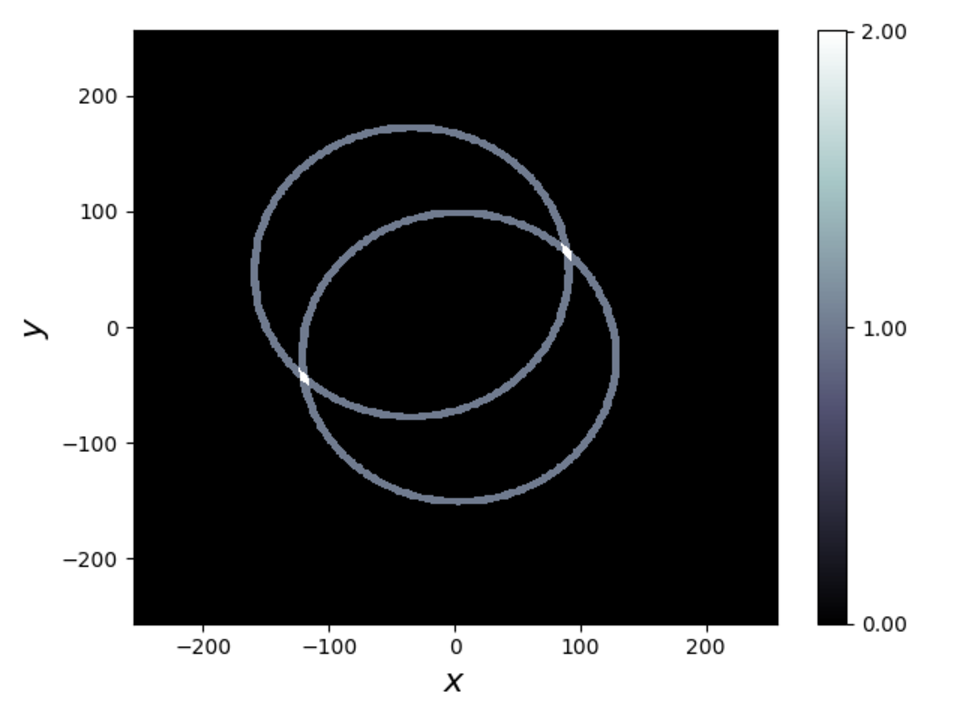
\includegraphics[height=0.45\textheight, trim={23mm 17mm 32mm 6mm}, clip]{truth}
\\ {\footnotesize Phantom}
\end{column}
\begin{column}{0.3\textwidth}
\centering
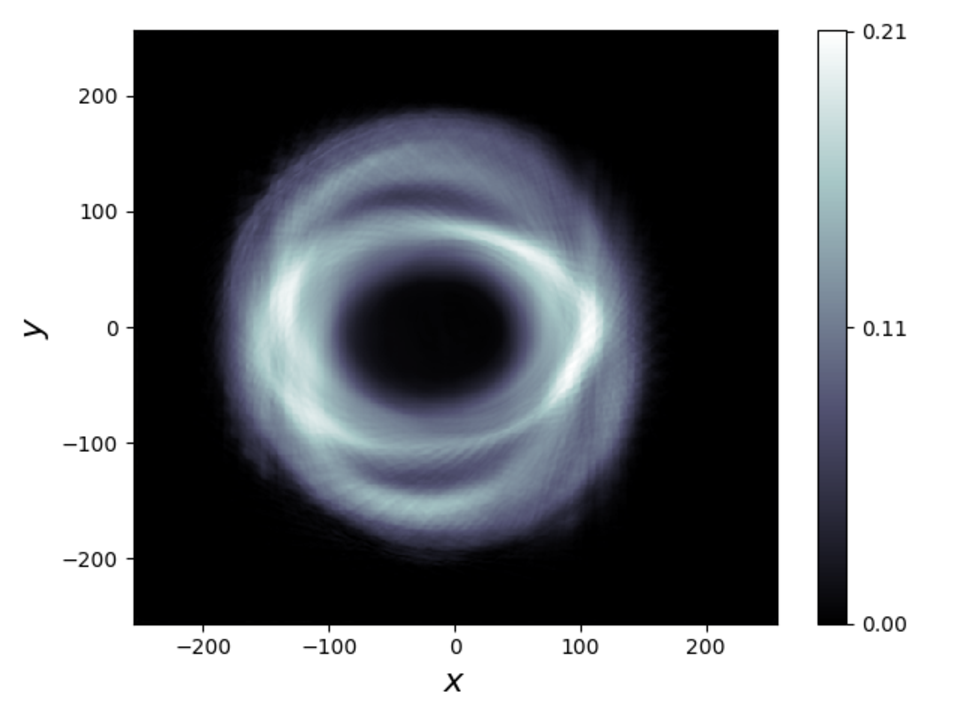
\includegraphics[height=0.45\textheight, trim={23mm 17mm 32mm 6mm}, clip]{learned_l2}
\\ {\footnotesize Using $L^2$-loss}
\end{column}
\begin{column}{0.3\textwidth}
\centering
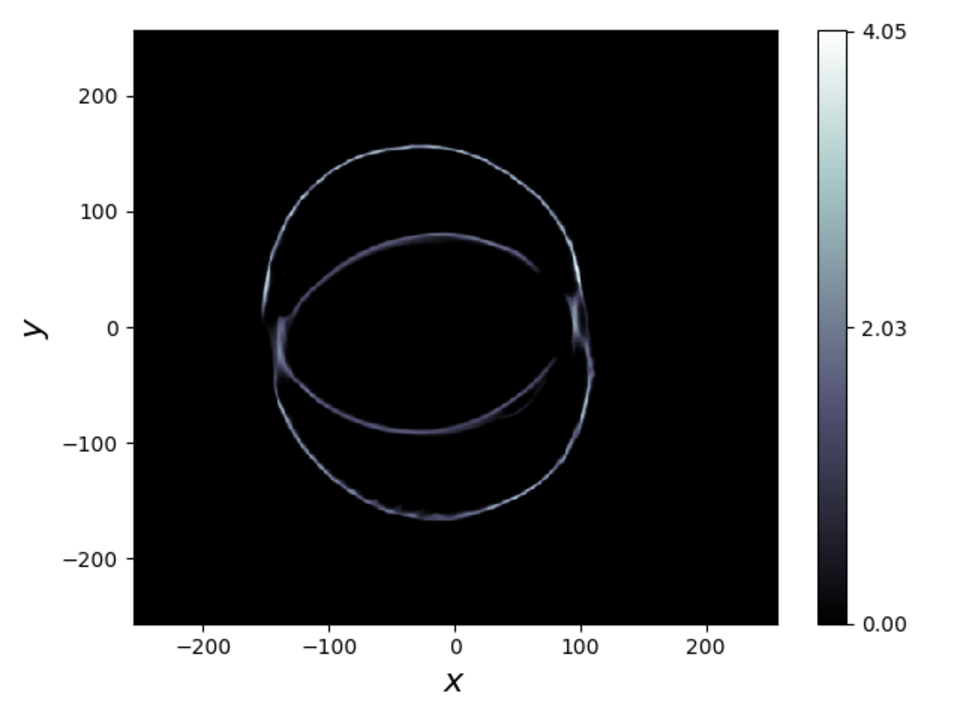
\includegraphics[height=0.45\textheight, trim={23mm 17mm 32mm 6mm}, clip]{learned_wasserstein}
\\ {\footnotesize Using OMT-loss}
\end{column}
\end{columns}
\par\bigskip
Learned Primal-Dual reconstructions when trained against misaligned training data using two loss functions:
\begin{itemize}
\item OMT-loss recovers `shape' but not position/orientation \cite{Adler:2017ab}.
\item $L^2$-loss recovers neither `shape' nor position/orientation \cite{Adler:2018aa}.
\end{itemize}
\end{frame}


% New frame
\begin{frame}{Integrating machine learning with inverse problems}
\begin{overprint}
\onslide<1> %% Slide 1: Overview
Approaches differ based on the type of training data, but all share following common traits:
\begin{itemize}
\item Fixed parametrisation $\{ \model{\param} \}_{\param}$ of reconstruction operators $\model{\param} \colon \DataSpace \to \RecSpace$
  by deep neural network.
\item Find optimal $\param^*$ by training/learning.
\item Use learned iterative method to embed data model (forward operator $\ForwardOp \colon \RecSpace \to \DataSpace$ and 
  data discrepancy $\DataLogLikelihood \colon \DataSpace \times \DataSpace \to \Real$) into deep neural network architecture 
  $\{ \model{\param} \}_{\param}$.
\item Possible to use (partially) learned forward operator.  
\end{itemize}
\alert{Let type of training data guide which approach to use!}
\onslide<2> %% Slide 2
\begin{itemize}
\item \structure{Supervised learning} % Supervised learning
  \begin{itemize}
  \item \structure{Statistical model:} 
    $(\RecSpace \times \DataSpace)$-valued random variable $(\stsignal,\stdata) \sim \JointLaw$ such that 
    $\ForwardOp(\stsignal) \approx \stdata$.
  \item \structure{Training data:} $(\signal_i, \data_i) \in \RecSpace \times \DataSpace \implies \JointLawEmp$.
  \item \structure{Learning:} 
    Compute $\param^*\in \ParamSet$ by solving 
    \vskip-0.5\baselineskip
    \[  \param^* \in \argmin_{\param\in\ParamSet} \loss(\param)
       \quad\text{where}\quad
       \loss(\param) := \Expect_{\JointLawEmp} \Bigl[ \SignalDist\bigl( \model{\param}(\stdata), \stsignal\bigr) \Bigr].
    \]
    \vskip-0.5\baselineskip
  \item \structure{Usage:} $\model{\param^*} \colon \DataSpace \to \RecSpace$ can be used for reconstruction.  
  \end{itemize}
\item \structure{Supervised priors} % Supervised priors
  \begin{itemize}
  \item \structure{Statistical model:} 
    Know marginal distribution $\MargDistr{\stsignal}$ of $\RecSpace$-valued random variable $\stsignal$ generating $\signaltrue$.
  \item \structure{Training data:} $\signal_i \in \RecSpace \implies \MargDistrEmp{\stsignal}$.
  \item \structure{Learning:}  
    Learn a prior distribution $\RegFunc_{\param}(\signal) \approx -\log \bigl( \MargDistrEmp{\stsignal}(\signal) \bigr)$ for 
    $\signal \in \RecSpace$. 
  \item \structure{Usage:} 
    Use $\RegFunc_{\param} \colon \RecSpace \to \Real$ as regulariser, e.g., in a variational method.
  \end{itemize}
\end{itemize}
\onslide<3> %% Slide 3
\begin{itemize}
\item \structure{Unsupervised learning} % Supervised priors
  \begin{itemize}
  \item \structure{Statistical model:} 
    Closely related to supervised priors, know marginal distribution $\MargDistr{\stdata}$ of $\DataSpace$-valued random variable 
    $\stdata$ generating $\data$. Cannot learn a prior, but one can use maximum-likelihood to address computational complexity.
  \item \structure{Training data:} $\data_i \in \DataSpace \implies \MargDistrEmp{\stdata}$.
  \item \structure{Learning:} Compute $\param^*\in \ParamSet$ by solving 
    \[
      \param^* := \argmin_{\param\in \ParamSet} \loss(\param)
      \quad\text{with}\quad
      \loss(\param) :=
        \Expect_{\MargDistrEmp{\stdata}} \Bigl[ 
        \DataLogLikelihood\Bigl(\ForwardOp\bigl(\model{\param}(\stdata)\bigr), \stdata\Bigr) 
        + \RegFunc\bigl(\model{\param}(\stdata) \bigr) 
      \Bigr].
    \]
  \item \structure{Usage:} 
    Improves performance.
  \end{itemize}
\end{itemize}
\onslide<4> %% Slide 4
\begin{itemize}
\item \structure{Unpaired data} % Unpaired data
  \begin{itemize}
  \item \structure{Statistical model:} 
    One has is access to marginal distributions $\MargDistr{\stsignal}$ and  $\MargDistr{\stdata}$ for both $\stsignal$ and $\stdata$, respectively. 
    Can make combinations of the above, e.g., either first train a learned prior, and then use unsupervised learning to minimise it, or something 
    similar to CycleGAN \cite{Zhu:2017aa}.
  \item \structure{Training data:} $\signal_i \sim \RecSpace$ and $\data_i \in \DataSpace \implies \MargDistrEmp{\stsignal} \otimes \MargDistrEmp{\stdata}$.
  \item \structure{Learning:} Compute $\param^*_D, \param^*_C,\param^*$ by solving 
\begin{multline*}
  (\param^*_D, \param^*_C,\param^*) :=
  \argmax_{\param_D, \param_C} \biggl\{ \argmin_{\param}
    \Expect_{\MargDistrEmp{\stsignal} \otimes \MargDistrEmp{\stdata}}
    \biggl[
        \SignalDist\Bigl( 
      	  \model{\param}\bigl(\ForwardOp(\stsignal) \bigr),
      	  \stsignal
        \Bigr)
      +
      \mathcal{D}_{\param_D}(\stdata)
      -
      \mathcal{D}_{\param_D}\bigl(\ForwardOp(\stsignal)\bigr) 
    \\
   + \DataLogLikelihood\Bigl(
         \ForwardOp\bigl( \model{\param}(\stdata) \bigr),
         \stdata
      \Bigr)
      +
      \mathcal{C}_{\param_C}(\stsignal)
      -
      \mathcal{C}_{\param_C}\bigl(\model{\param}(\stdata) \bigr)
    \biggr] \biggr\}.
  \end{multline*}  
  In the above, $\mathcal{C}_{\param_C} \colon \RecSpace \to \Real$ and $\mathcal{D}_{\param_D} \colon \DataSpace \to \Real$ are 
  adversarial discriminators that try to distinguish generated signal/data from actual signal/data, respectively.
  \item \structure{Usage:} $\model{\param^*} \colon \DataSpace \to \RecSpace$ can be used for reconstruction.  
  \end{itemize}
\end{itemize}
\end{overprint}
\end{frame}


% New frame
\begin{frame}[plain]
\slideTitle{Task based reconstruction}
\begin{itemize}
\item Motivation
\item Functional analytic framework
\item Statistical framework
\item Examples
  \begin{itemize}
  \item Joint reconstruction and segmentation
  \item Joint reconstruction and image comparison
  \item Joint reconstruction and classification
  \end{itemize}
\end{itemize}
\end{frame}


% New frame
\begin{frame}{Motivation}
\begin{itemize}
\item \structure{Decision making related to task:}
Reconstruction often only one step in pipeline for decision making related to a task.
\begin{itemize}
\item Model parameters are typically summarised, either by an expert or by using specific descriptors, in an analysis step.
\item Summaries used as input for decision making.
\end{itemize}
\item \structure{Natural question:}
Can one adapt the reconstruction method for the specific task at hand? 
\item \structure{Task based reconstruction:}
Reconstruction methods that aim to integrate (parts of) decision making related to a task.
\\
Frequently also referred to as `end-to-end'.
\end{itemize}
\end{frame}

% New frame
\begin{frame}{Example: Radiomics}
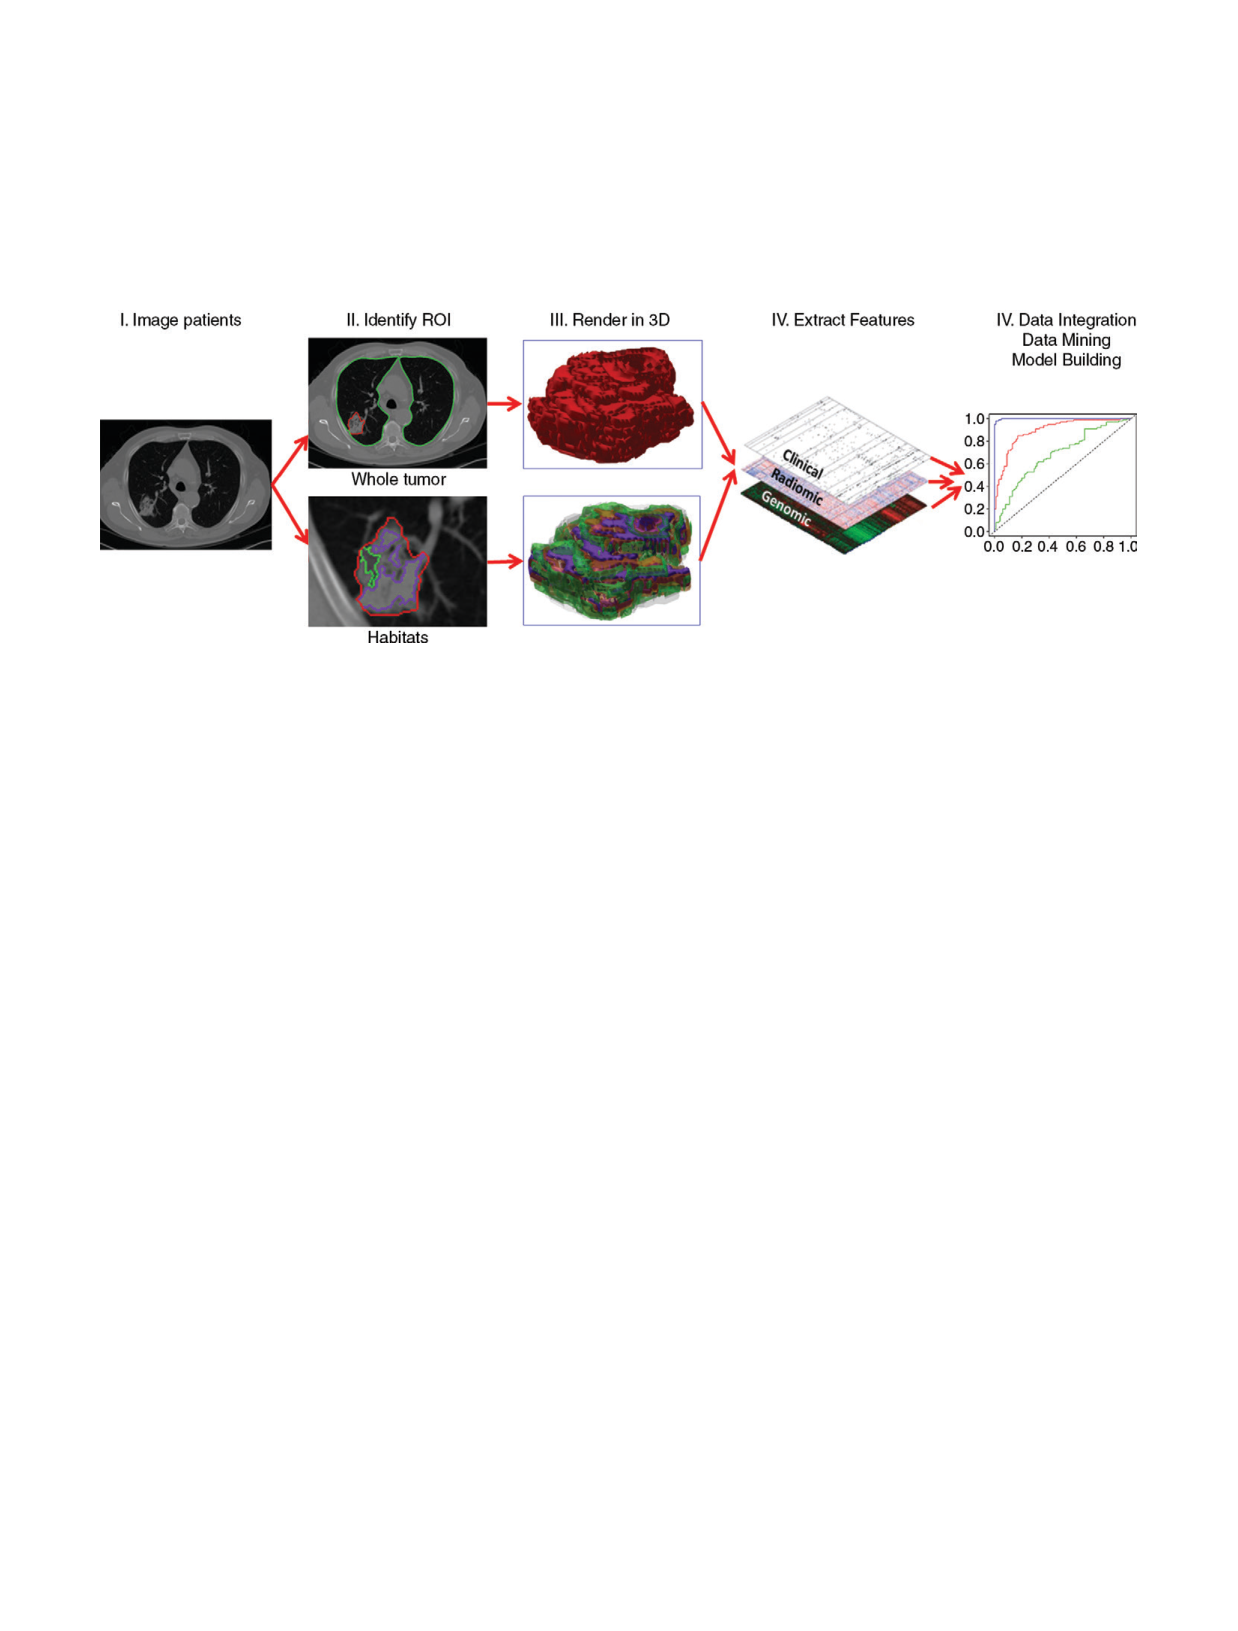
\includegraphics[width=\textwidth]{radiomics_pipeline}
\par\bigskip
Radiomics and its usage in decision support \cite{Gillies:2016aa}.
\end{frame}

% New frame
\begin{frame}{Typical workflow involving an inverse problem}
\begin{figure}
\centering
% Define block styles
\tikzstyle{decision} = [diamond, draw, fill=blue!20, 
    text width=4.5em, text badly centered, node distance=3cm, inner sep=0pt]
\tikzstyle{block} = [rectangle, draw, fill=blue!20, 
    text width=6.7em, text centered, rounded corners, minimum height=4em]
\tikzstyle{line} = [draw, -latex']
\tikzstyle{cloud} = [draw, ellipse,fill=red!20, node distance=3cm,
    minimum height=4em]
\begin{tikzpicture}[node distance = 0.23\linewidth, auto,scale=0.85, every node/.style={scale=0.85}]
    % Place nodes
    % Row 1
    \node [block] (device) {Data acquisition device};
    \node [cloud, left of=device, node distance = 0.35\linewidth] (sample) {Sample};
    \node [block, right of=device, node distance = 0.35\linewidth] (preprocess) {Data pre-processing};
    % Row 2
    \node [block, below of=preprocess] (reconstruction) {Reconstruction};
    \node [block, left of=reconstruction, node distance = 0.35\linewidth] (postprocess) {Feature extraction};
    \node [block, left of=postprocess, node distance = 0.35\linewidth] (model building) {Model building};
    % Row 3
    \node [cloud, below of=model building] (scientist) {End user};
    % Draw edges
    \path [line] (sample) -- node[align=left] {Sample \\ preparation} (device);
    \path [line] (device) -- node[align=left] {Raw \\ data} (preprocess);
    \path [line] (preprocess) -- node[align=left] {Cleaned \\ data} (reconstruction);
    \path [line] (reconstruction) -- node[above,align=left] {Signal} (postprocess);
    \path [line] (postprocess) -- node[above,align=left] {Extracted \\ features} (model building);
    \path [line] (model building) -- node[align=left] {Task related \\ model} (scientist);
    % Highlight region
     \visible<2>{\fill[overlay,red,fill opacity=0.4] (-6.5,-4.25) rectangle (6.5,-2.2);}
\end{tikzpicture}
\end{figure}
\end{frame}

% New frame
\begin{frame}{Functional analytic framework}
\begin{itemize}
\item \structure{Inverse problem:}
Recover model parameters $\signaltrue \in \RecSpace$ given data $\data \in \DataSpace$ were $\data = \ForwardOp(\signaltrue) + \datanoise$. 
\begin{itemize}
\item $\ForwardOp \colon \RecSpace \to \DataSpace$ forward operator 
\item $\datanoise \in \DataSpace$ sample of $\DataSpace$-valued random variable $\stdatanoise \sim \noisedist$.
\end{itemize}
\visible<2->{
\item \structure{Feature reconstruction:}
As above, but goal is to recover features $\decision \in \DecisionSpace$ given data $\data \in \DataSpace$ and $\featuremap \colon \RecSpace \to \DecisionSpace$ (task related feature extraction operator) where:
\begin{columns}[c]
\begin{column}{0.4\textwidth}
Need to find the dotted operator.
\end{column}
\begin{column}{0.3\textwidth}
\hskip-0.5\columnwidth
\begin{tikzpicture}[ampersand replacement=\&]
\begin{tikzcd}[column sep=large,row sep=large]
 \RecSpace \arrow[r, "\ForwardOp"] \arrow[swap, d, "\featuremap"] \& 
 \DataSpace \arrow[ld, dotted] \\
 \DecisionSpace \&
\end{tikzcd}
\end{tikzpicture}
\end{column}
\end{columns}
}
\visible<3->{
\item $\featuremap$ often highly non-injective, makes no sense to consider $\ForwardOp \circ \featuremap^{-1} \colon \DecisionSpace \to \DataSpace$ as `new forward operator'.
}
\end{itemize}
\end{frame}

% New frame
\begin{frame}{Functional analytic framework}{Examples from tomography}
\begin{overprint}
\onslide<1-3>
\begin{itemize}
\visible<1->{
\item \structure{Edge reconstruction}
\begin{itemize}
  \item Lambda tomography \cite{Krishnan:2015aa}.
  \item Variational regularisation using TV-type of regularisers \cite{Burger:2013aa}.
  \item Sparse regularisation w.r.t. learned or analytic (curvelets, shearlets, beamlets, bandlets, \ldots) dictionary
    \cite{Foucart:2013aa,Rubinstein:2010aa,Kutyniok:2012aa}.
\end{itemize}
}
\visible<2->{
\item \structure{Joint reconstruction and segmentation}
\begin{itemize}
  \item Approximate inverse with segmentation operator \cite{Louis:2011aa}.
  \item Variational regularisation using Mumford-Shah penalty \cite{Ramlau:2007aa,Hohm:2015aa}.
  \item Level set approaches \cite{Yoon:2010aa}.
\end{itemize}
}
\visible<3->{
\item \structure{Joint reconstruction and pixel classification (labelling)}
\begin{itemize}
  \item MAP estimation using Gauss-Markov-Potts priors \cite{Mohammad-Djafari:2009aa,Romanov:2016aa}
\end{itemize}  
}
\end{itemize}  
\onslide<4->
\visible<4->{
\begin{itemize}  
\item \structure{Joint reconstruction and (non-rigid) image registration}
\begin{itemize}
  \item Optical flow based methods \cite{Burger:2017aa}.
  \item LDDMM based diffeomorphic deformations \cite{Chen:2018aa}.
  \item Optimal transport priors \cite{Karlsson:2017aa}.
\end{itemize}
\end{itemize}    
}
\end{overprint} 
\end{frame}

% New frame
\begin{frame}{Functional analytic framework}{Summary}
\structure{State-of-the-art approaches:}
  Based on variational methods, which have some serious drawbacks.
  \begin{itemize}
  \item Computationally unfeasible
  \item Can only handle `simple' features that need further processing before usage in decision making.
  \item Single estimator of feature often inadequate for decision making, need to recover the feature along with its uncertainty. 
  \end{itemize}
\end{frame}

% New frame
\begin{frame}{Statistical framework}
\begin{itemize}
\item \structure{Setting}
\begin{itemize}
\item $\RecSpace$ space of model parameters, $\stsignal$ is $\RecSpace$-valued random variable generating $\signaltrue \in \RecSpace$
\item $\DataSpace$ space of data, $\stdata$ is $\DataSpace$-valued random variable generating data: $\stdata = \ForwardOp(\stsignal) + \stdatanoise$
\item $\DecisionSpace$ space of (task related) decisions, $\stdecision$ is $\DecisionSpace$-valued random variable generating task related decisions. 
\visible<4->{\item Training data: Samples $(\signal_i,\data_i,\decision_i)$ of $(\stsignal,\stdata,\stdecision)$.}
\end{itemize}
\visible<2->{\item \structure{Operators}
\begin{itemize}
\item Parametrised reconstruction: $\model{\signalpara} \colon \DataSpace \to \RecSpace$
\item Parametrised task operator: $\TaskOpLearned{\taskpara} \colon \RecSpace \to \DecisionSpace$
\item Task based reconstruction: 
$\TaskOpLearned{\taskpara} \circ \model{\signalpara} \colon \DataSpace \to \DecisionSpace$
\end{itemize}
}
\visible<3->{\item \structure{Distance notions:} 
\vskip-\baselineskip
\[
 \DistFunc{\RecSpace} \colon \RecSpace \times \RecSpace \to \Real \quad\text{and}\quad
 \DecisionDist \colon \DecisionSpace \times \DecisionSpace \to \Real 
\] 
}
\visible<4->{
\item \vskip-\baselineskip \structure{Joint training:} 
Determine $(\signalpara,\taskpara)$ by minimising \alert{joint} expected loss (risk) against training data
{\small
\begin{equation*}
  \JointRisk(\signalpara,\taskpara) 
       = \Expect_{(\stsignal,\stdata,\stdecision)}\Bigl[            
            C_1 \DistFunc{\RecSpace}\bigl( \model{\signalpara}(\stdata),
            \stsignal \bigr) 
            + 
            C_2 \DecisionDist\bigl( \TaskOpLearned{\taskpara} \circ \model{\signalpara}(\stdata),
            \stdecision \bigr) 
          \Bigr] 
\end{equation*}
}       
}
\end{itemize}
\end{frame}


% New frame
\begin{frame}{Task based reconstruction}{Computational framework}
\begin{itemize}
\item \structure{Flexibility:} Possible to \alert<1>{jointly set} $\signalpara$ and $\taskpara$
\item \structure{Computational complexity:} 
  Possible to apply task based reconstruction $\TaskOpLearned{\taskpara} \circ \model{\signalpara}$ on large-scale problems.
\end{itemize}
\visible<2->{
\begin{itemize}
\item $\model{\signalpara} \colon \DataSpace \to \RecSpace$ given by \alert<2>{learned iterative reconstruction}.\\[0.35em]
\item $\TaskOpLearned{\taskpara} \colon \RecSpace \to \DecisionSpace$ typically given by off-the shelf machine learning method relevant for 
  the task (without reconstruction step): 
  \begin{itemize}
  \item segmentation
  \item image comparison
  \item classification
  \end{itemize}
}  
\end{itemize}
\visible<3->{
\structure{Pre-training:} If there are training data $\tData_1 \subset \RecSpace \times \DataSpace$ and 
$\tData_2 \subset \RecSpace \times \DecisionSpace$, then we can pre-train to learn preliminary values:
\begin{alignat*}{3}
  \tData_1 &\,\,\,\Longrightarrow\,\,\, \signalpara^* \in \SignalParamSpace 
    &\,\,\,\Longrightarrow\,\,\,& \model{\signalpara^*} \colon \DataSpace \to \RecSpace \\
  \tData_2 &\,\,\,\Longrightarrow\,\,\, \taskpara^* \in \taskparamSpace 
    &\,\,\,\Longrightarrow\,\,\,& \TaskOpLearned{\taskpara^*} \colon \RecSpace \to \DecisionSpace
\end{alignat*}
}
\end{frame}

% New frame
\begin{frame}[plain]
\begin{center}
{\Large \structure{Examples of task based reconstruction}}
\end{center}
  \begin{itemize}
  \item Joint reconstruction and segmentation
  \item Joint reconstruction and image comparison
  \item Joint reconstruction and classification
  \end{itemize}
\end{frame}

% New frame
\begin{frame}{Joint reconstruction and segmentation}
\begin{overprint}
\onslide<1>
\structure{Task based reconstruction problem:} Recover probability map of segmented part of the attenuation coefficient from a sinogram (tomographic data)
\[
\data = \ForwardOp(\signal) + \datanoise
\]
\begin{itemize}
\item Forward operator: 2D ray transform 
\item Geometry: Parallel beam, 183 lines/angle, 30 angles
\item Noise: 0.1\% additive Gaussian
\item Image: $128 \times 128$ pixel 
\item Training data: 100 triplets $(\signal_i,\data_i,\decision_i)$ where $\decision_i$ is the segmentation (binary image).
\\
Extended with data argumentation ($\pm 5$ pixel translation and $\pm 10^{\circ}$ rotation).
\end{itemize}
\onslide<2-4>
\begin{itemize}
\item \structure{Learned reconstruction $\model{\signalpara} \colon \DataSpace \to \RecSpace$}
\cite{Adler:2018aa}
\begin{itemize}
\item Learned primal dual
\item Distance: $\DistFunc{\RecSpace}$ is $L^2$-distance on $\RecSpace$
\end{itemize}
\visible<3->{
\item \structure{Learned task operator $\TaskOpLearned{\taskpara} \colon \RecSpace \to \DecisionSpace$}
  \cite{Ronneberger:2015aa}.
\begin{itemize}
\item $\DecisionSpace =$ probability distributions over binary images on $\domain$, i.e., 
  grey-scale images with values in $[0,1]$ that gives probability that point is in segmented object.
\item $\TaskOpLearned{\taskpara}$ given by `off the shelf' U-net convolutional neural net architecture for segmentation
\item Distance: $\DecisionDist$ is cross entropy
\end{itemize}
}
\visible<4->{
\item \structure{Task based reconstruction
$\TaskOpLearned{\taskpara} \circ \model{\signalpara} \colon \DataSpace \to \DecisionSpace$}
\begin{itemize}
\item No pre-training
\item Joint risk: Case with $C_1=C$ and $C_2=1$, so 
\[  \JointRisk(\signalpara,\taskpara) 
       = \Expect_{(\stsignal,\stdata,\stdecision)}\Bigl[            
            C \, \SignalDist(\signalpara) + \DecisionDist(\taskpara)
          \Bigr] 
\]
\end{itemize}
}
\end{itemize}
\end{overprint}
\end{frame}

% New frame
\begin{frame}{Joint reconstruction and segmentation}
%\onslide<1> %% Slide 1
\begin{tikzpicture}
\begin{axis}[
  height=0.4\textheight,
  width=0.9\textwidth,
  x label style={at={(axis description cs:1,0.35)},anchor=north,xshift=0.2cm},
  xlabel=$C$,
  xmode=log,
  log basis x={10},  
  ylabel style={yshift=0.3cm,rotate=-90},  
%  ylabel near ticks,  
  ylabel=$\SignalDist$,  
  ymode=log,
  log basis y={10}
]  
\addplot table [y=SLoss, x=C, col sep=comma]{rec_seg_data.txt};
\end{axis}
\end{tikzpicture} 
\\[0.75em]
\begin{tikzpicture}
\begin{axis}[
  height=0.42\textheight,
  width=0.9\textwidth,
  x label style={at={(axis description cs:1,0.35)},anchor=north,xshift=0.2cm},
  xlabel=$C$,
  xmode=log,
  log basis x={10},
  ylabel style={yshift=0.3cm,rotate=-90},  
%  ylabel near ticks,
  ylabel=$\DecisionDist$,
  ymode=log,
  log basis y={10}
]  
\addplot table [y=DLoss, x=C, col sep=comma]{rec_seg_data.txt};
\end{axis}
\end{tikzpicture}
\\[0.75em]
\begin{tikzpicture}
\begin{axis}[
  height=0.42\textheight,
  width=0.9\textwidth,
  x label style={at={(axis description cs:1,0.35)},anchor=north,xshift=0.2cm},
  xlabel=$C$,
  xmode=log,
  log basis x={10},  
  ylabel style={yshift=0.4cm,rotate=-90},  
%  ylabel near ticks,  
  ylabel=$\JointLoss$,  
  ymode=log,
  log basis y={10}
]  
\addplot table [y=JointLoss, x=C, col sep=comma]{rec_seg_data.txt};
\end{axis}
\end{tikzpicture} 
% Rent teoretiskt borde C -> \infty svara mot att man g�r segmenteringen efter�t.
\end{frame}

% New frame
\begin{frame}[plain]
\begin{columns}
\begin{column}{0.5\textwidth}
\begin{center}
Phantom \\[0.5em]
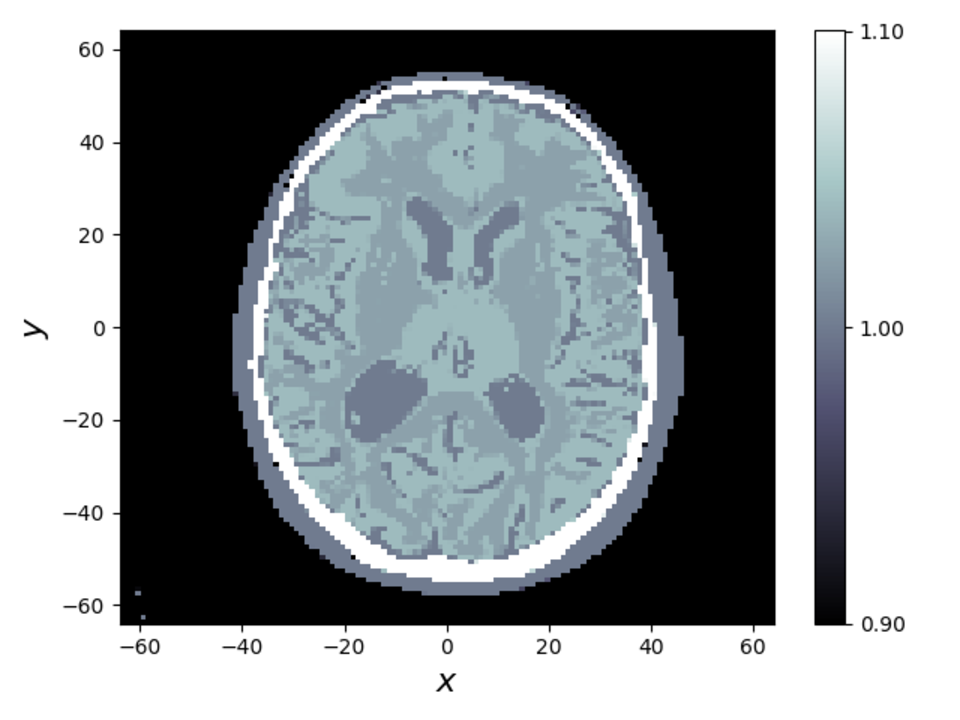
\includegraphics[height=0.47\textheight, trim={23mm 16mm 27mm 6mm}, clip]{result_true} 
\\[0.15em]
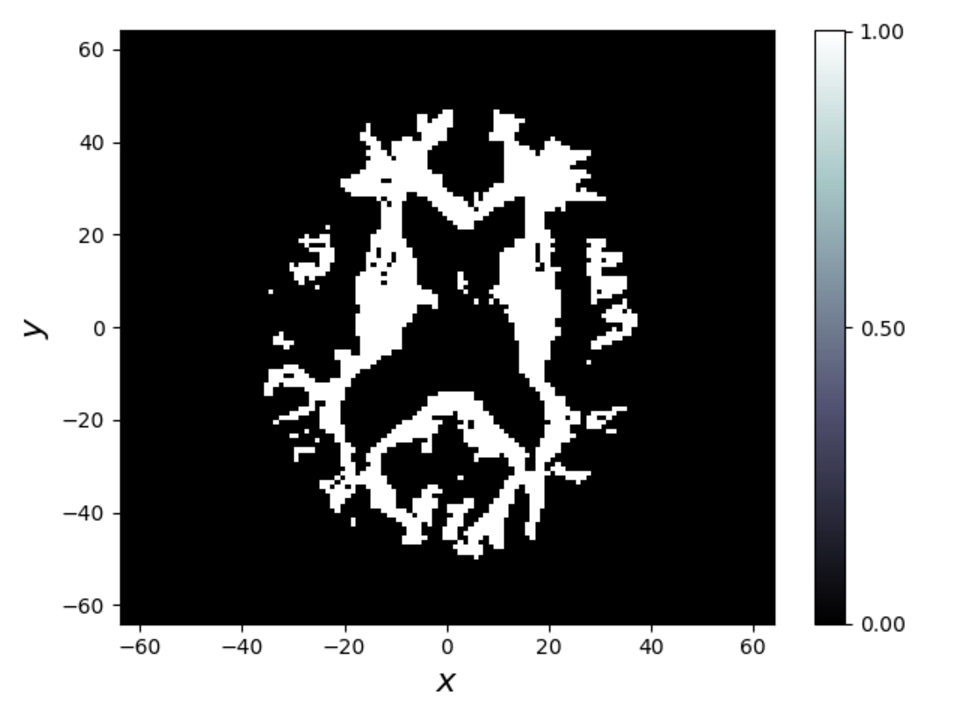
\includegraphics[height=0.47\textheight, trim={23mm 16mm 27mm 6mm}, clip]{segment_true} 
\end{center}
\end{column}
\begin{column}{0.5\textwidth}
\begin{center}
\begin{overprint}
\onslide<2> %% Slide 2
\hskip0.25\linewidth $C=0.01$ \\[0.5em]
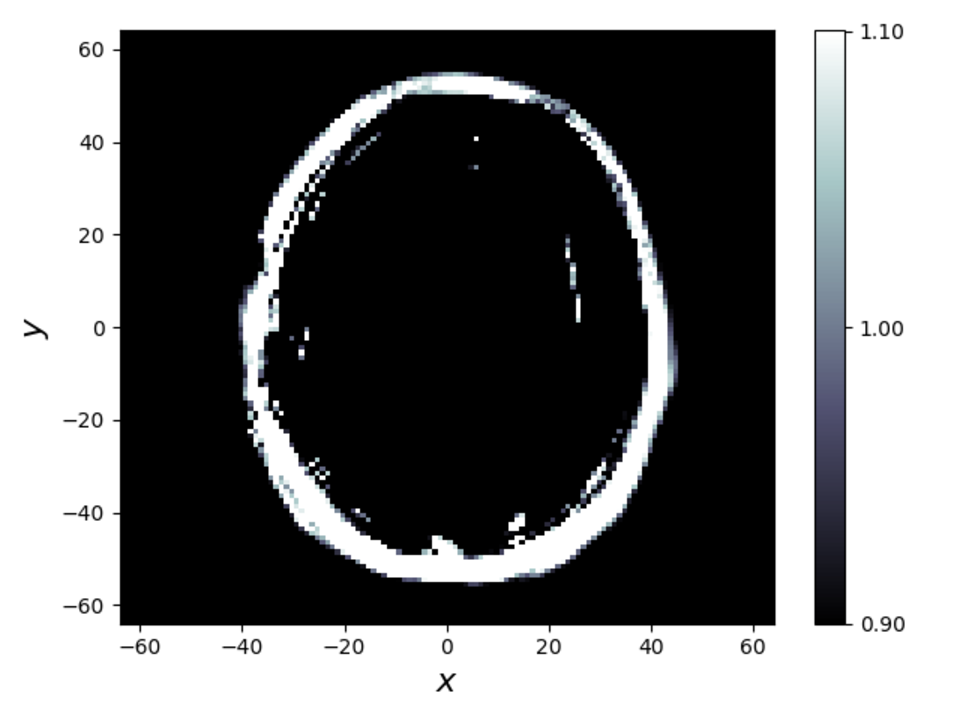
\includegraphics[height=0.47\textheight, trim={23mm 16mm 27mm 6mm}, clip]{result_0_01} 
\\[0.15em]
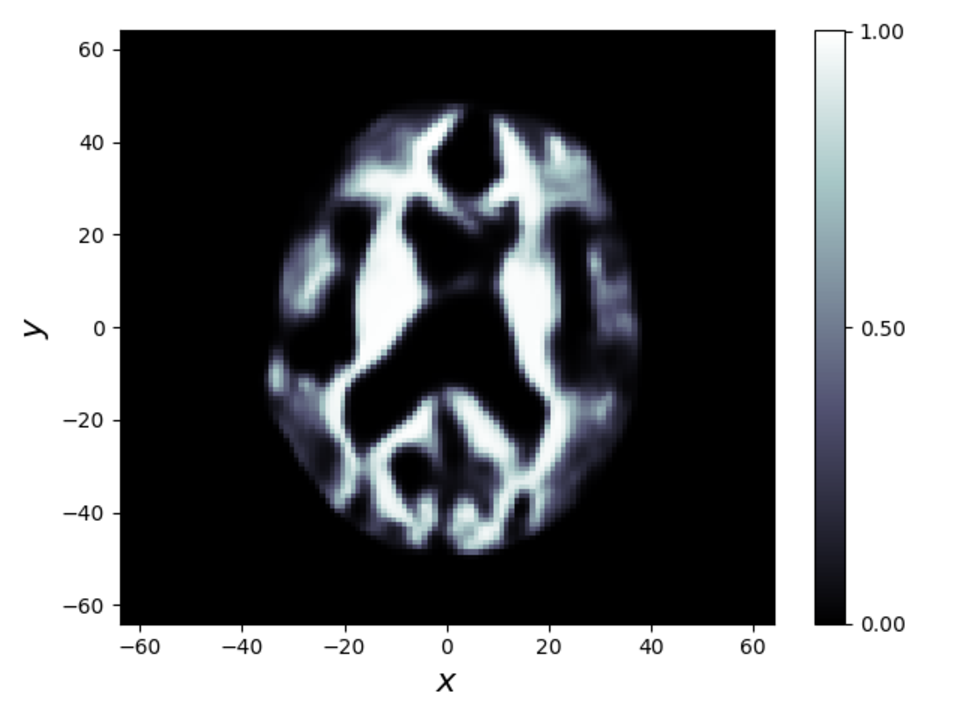
\includegraphics[height=0.47\textheight, trim={23mm 16mm 27mm 6mm}, clip]{segment_0_01} 
\onslide<3> %% Slide 3
\hskip0.25\linewidth $C=0.10$ \\[0.5em]
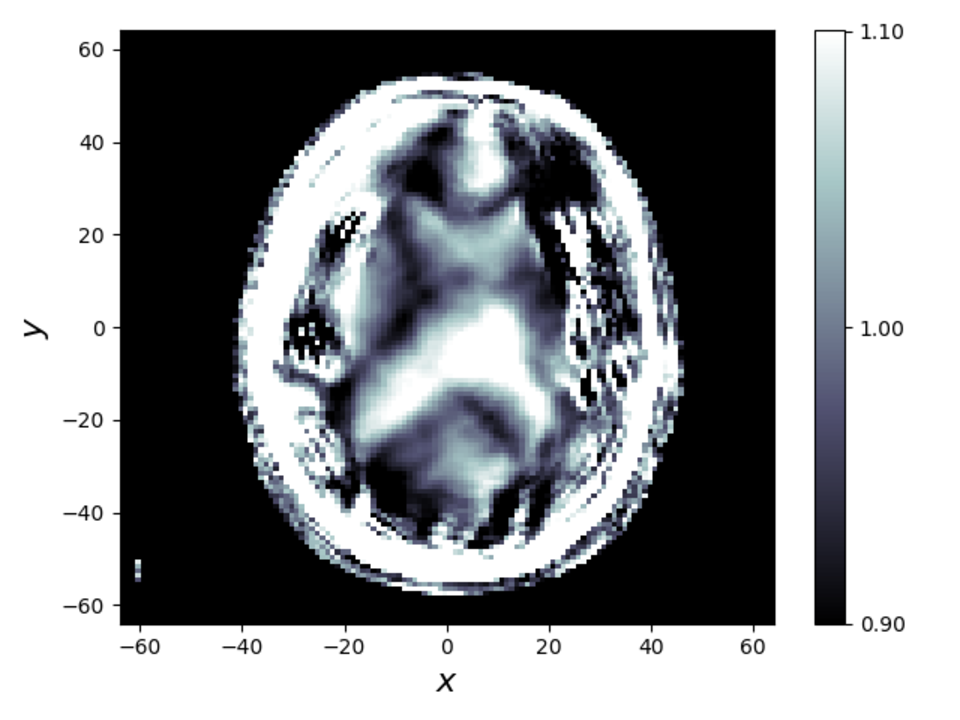
\includegraphics[height=0.47\textheight, trim={23mm 16mm 27mm 6mm}, clip]{result_0_10} 
\\[0.15em]
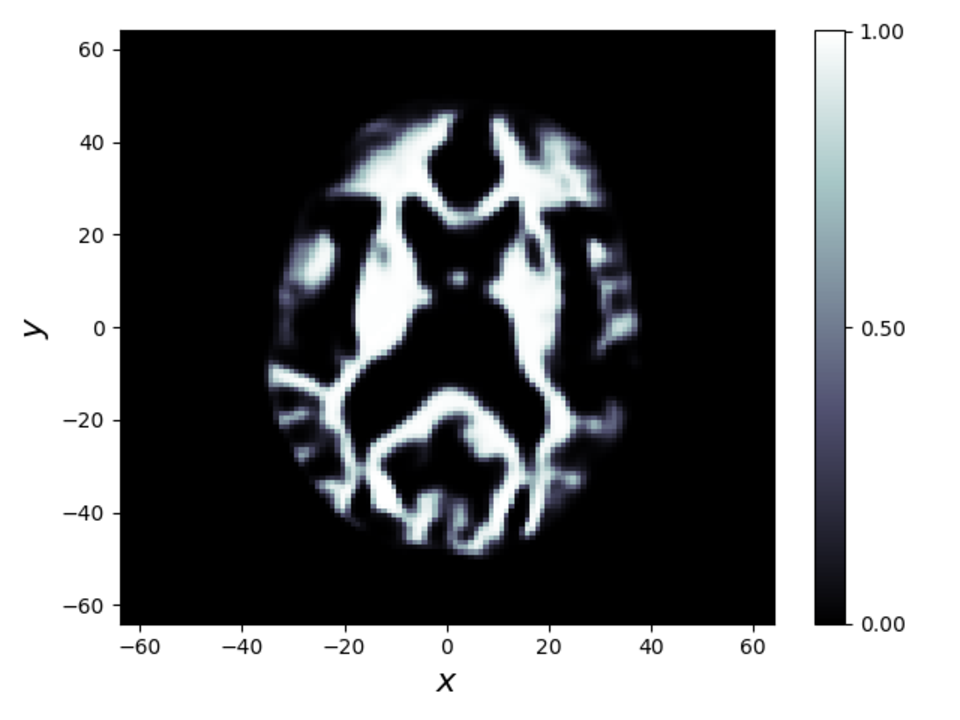
\includegraphics[height=0.47\textheight, trim={23mm 16mm 27mm 6mm}, clip]{segment_0_10} 
\onslide<4> %% Slide 4
\hskip0.25\linewidth $C=1.0$ \\[0.5em]
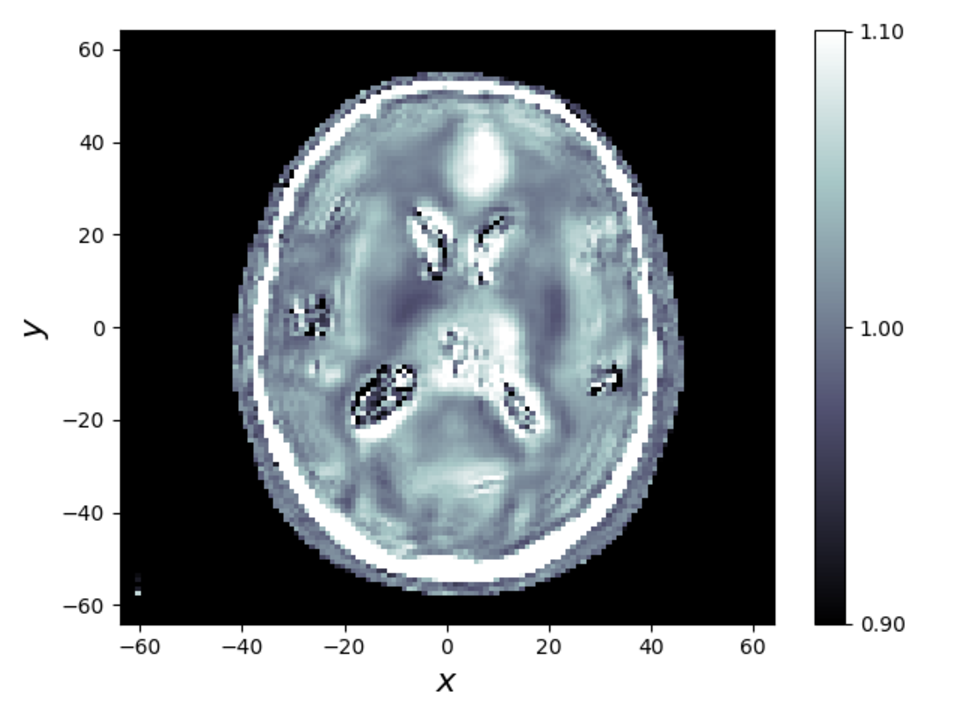
\includegraphics[height=0.47\textheight, trim={23mm 16mm 27mm 6mm}, clip]{result_1_0} 
\\[0.15em]
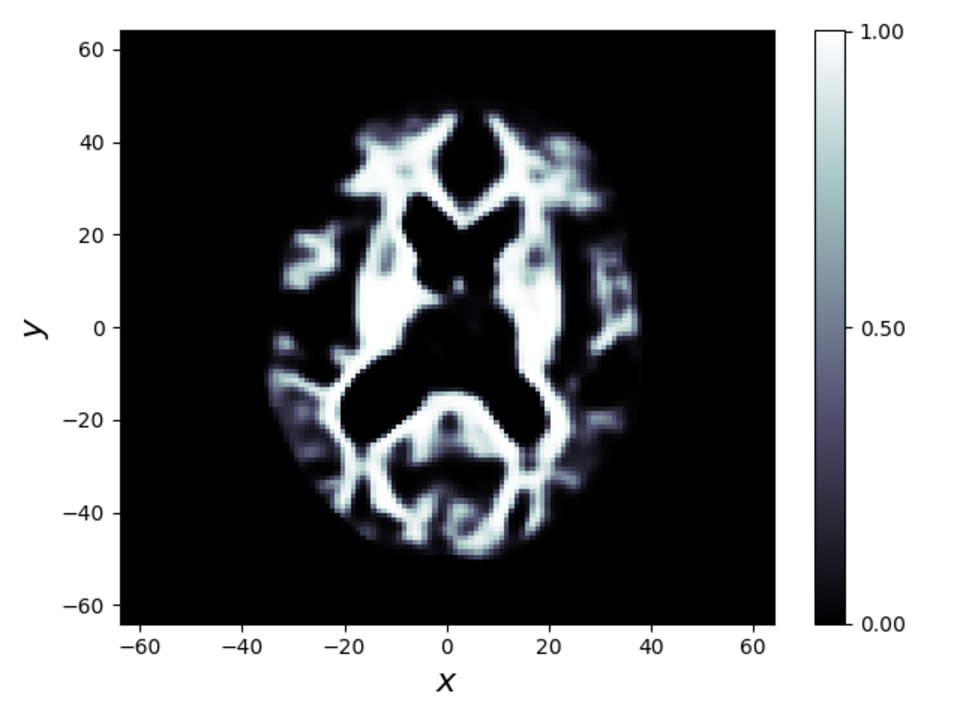
\includegraphics[height=0.47\textheight, trim={23mm 16mm 27mm 6mm}, clip]{segment_1_0} 
\onslide<5> %% Slide 5
\hskip0.25\linewidth $C=10.0$ \\[0.5em]
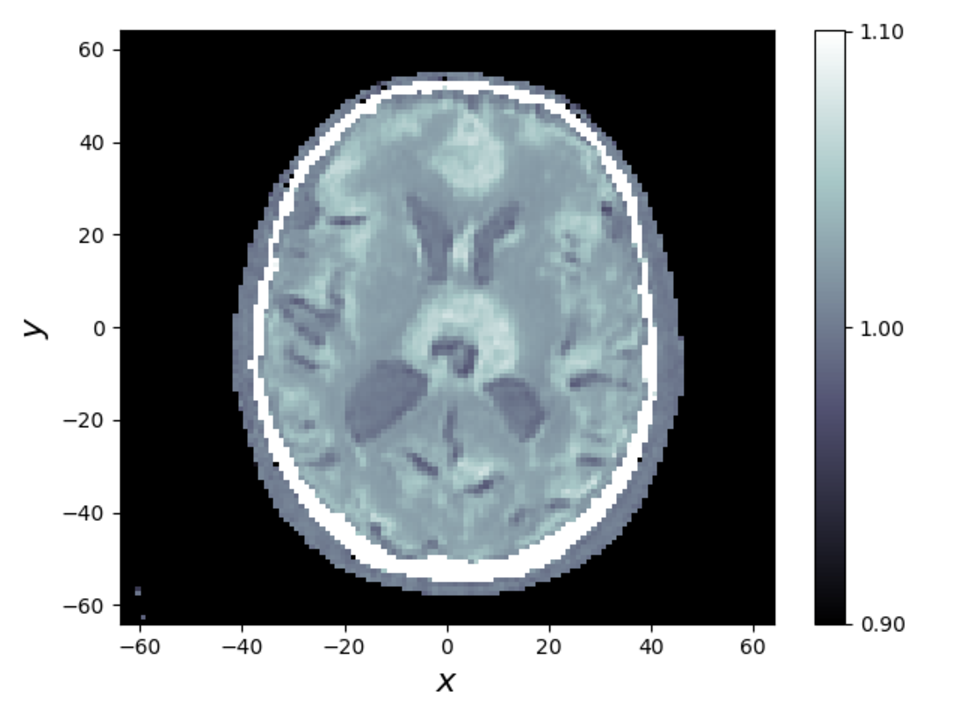
\includegraphics[height=0.47\textheight, trim={23mm 16mm 27mm 6mm}, clip]{result_10_0} 
\\[0.15em]
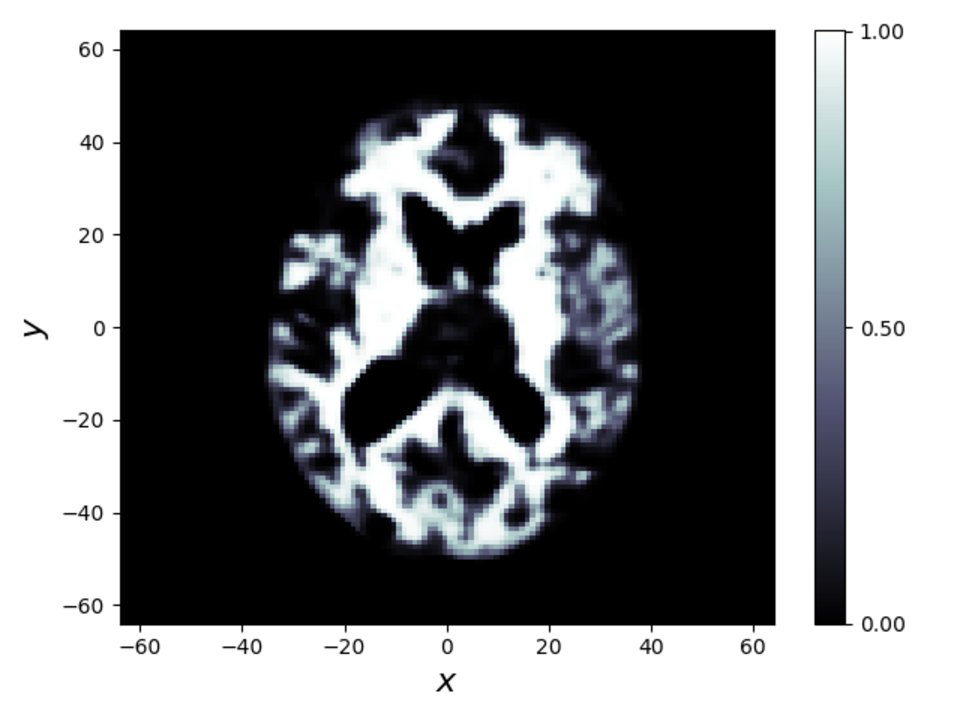
\includegraphics[height=0.47\textheight, trim={23mm 16mm 27mm 6mm}, clip]{segment_10_0} 
\onslide<6> %% Slide 6
\hskip0.25\linewidth $C=100.0$ \\[0.5em]
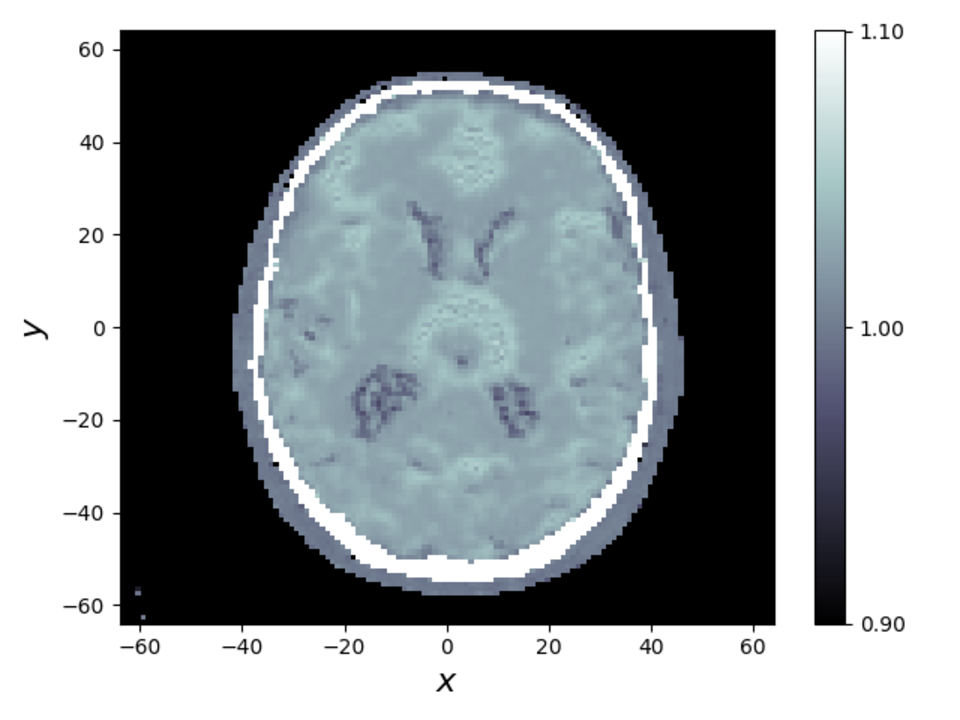
\includegraphics[height=0.47\textheight, trim={23mm 16mm 27mm 6mm}, clip]{result_100_0} 
\\[0.15em]
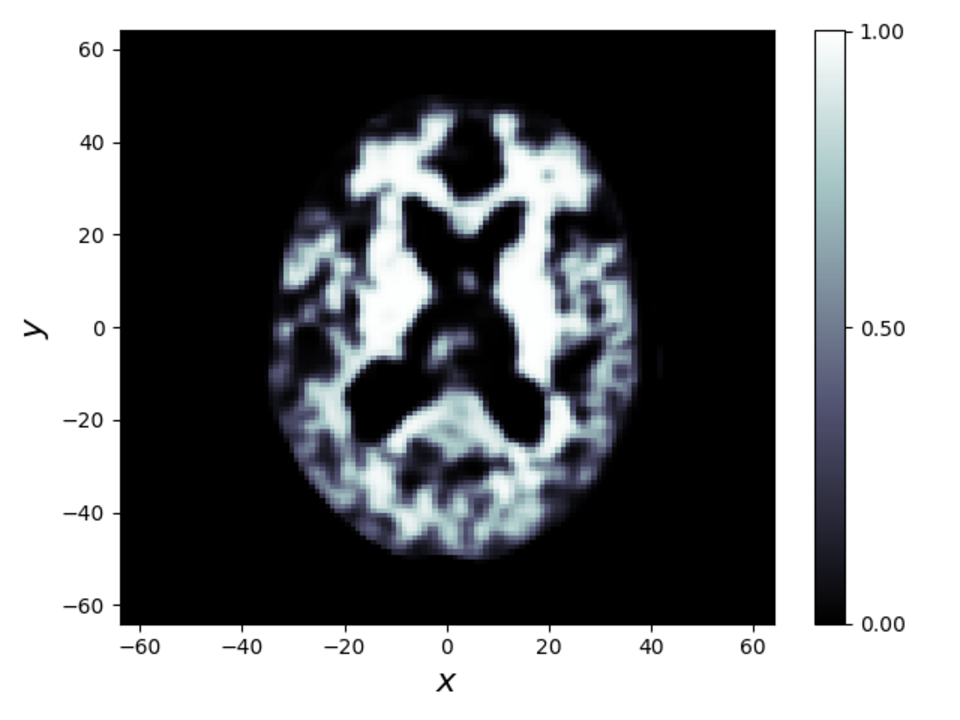
\includegraphics[height=0.47\textheight, trim={23mm 16mm 27mm 6mm}, clip]{segment_100_0} 
\onslide<7> %% Slide 7
\hskip0.25\linewidth $C=1000.0$ \\[0.5em]
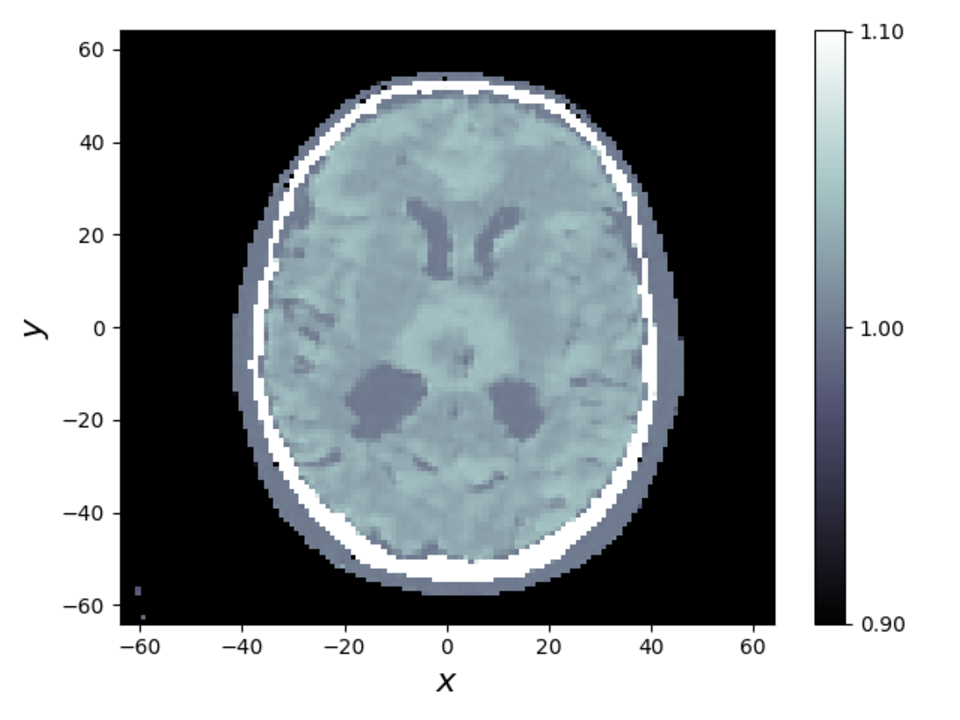
\includegraphics[height=0.47\textheight, trim={23mm 16mm 27mm 6mm}, clip]{result_1000_0} 
\\[0.15em]
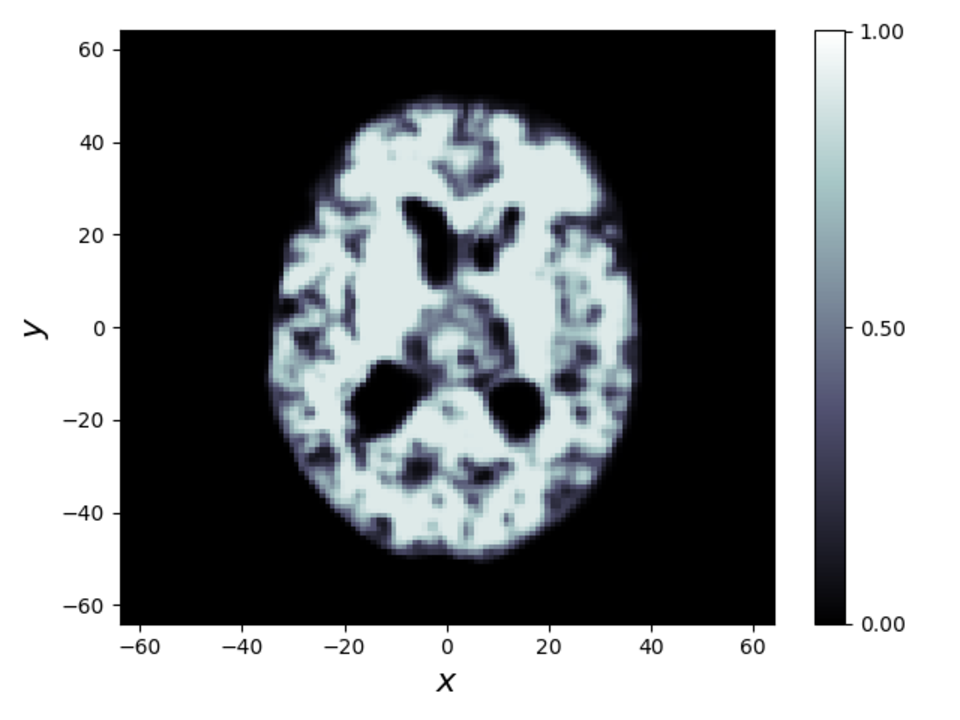
\includegraphics[height=0.47\textheight, trim={23mm 16mm 27mm 6mm}, clip]{segment_1000_0} 
\end{overprint}
\end{center}
\end{column}
\end{columns}
\end{frame}

% New frame
\begin{frame}{Joint reconstruction and image comparison}
\begin{overprint}
\onslide<1>
\structure{Task based reconstruction problem:} Recover the difference map for the attenuation coefficient in two images from their sinograms (tomographic data)
\[
\data_1 = \ForwardOp(\signal_1) + \datanoise_1
\quad\text{and}\quad
\data_2 = \ForwardOp(\signal_2) + \datanoise_2
\]
\vskip-0.5\baselineskip
\begin{itemize}
\item Forward operators: 2D ray transform 
\item Geometries: Parallel beam, 183 lines/angle, 30 angles
\item Noise: 0.1\% additive Gaussian
\item Images: $128 \times 128$ pixel 
\item Training data: Triplets 
$\bigl( (\signal^1_i,\signal^2_i), (\data^1_i, \data^2_i), \decision_i \bigr)$ where $\decision_i := \signal^1_i-\signal^2_i$.
\end{itemize}
\onslide<2-4>
\begin{itemize}
\item \structure{Learned reconstruction $\model{\signalpara} \colon \DataSpace \times \DataSpace  \to \RecSpace \times \RecSpace$}
\cite{Adler:2018aa}.
\begin{itemize}
\item Learned primal dual in each channel
\item Distance: $\DistFunc{\RecSpace}$ is sum of channel-wise $L^2$-distances on $\RecSpace$.
\end{itemize}
\visible<3->{
\item \structure{Task operator $\TaskOpLearned{\taskpara} \colon \RecSpace \times \RecSpace \to \DecisionSpace$}
\begin{itemize}
\item $\DecisionSpace$ real-valued functions (difference images) defined on $\domain$.
\item $\TaskOpLearned{\taskpara}(\signal_1,\signal_2) = $ U-net that maps pair of images in $\RecSpace$ to an image in $\DecisionSpace$ (no probabilities).
\item Distance: $\DecisionDist$ is $L^2$-distance
\end{itemize}
}
\visible<4->{
\item \structure{Task based reconstruction
$\TaskOpLearned{\taskpara} \circ \model{\signalpara} \colon \DataSpace \times \DataSpace \to \DecisionSpace$}
\begin{itemize}
\item No pre-training
\item Joint risk: Case with $C_1=C$ and $C_2=1$, i.e., 
\[  \JointRisk(\signalpara,\taskpara) =
      \Expect\Bigl[ 
         C\,\SignalDist(\signalpara) +
         \Bigr\Vert 
              \TaskOpLearned{\taskpara}\bigr( 
                 \model{\signalpara}(\stdata_1,\stdata_2)
               \bigr) - (\stsignal_1-\stsignal_2)
           \Bigr\Vert_2
         \Bigr]
\]
\end{itemize}
}
\end{itemize}
\end{overprint}
\end{frame}

% New frame
\begin{frame}{Joint reconstruction and image comparison}
\begin{tikzpicture}
\begin{axis}[
  height=0.4\textheight,
  width=0.9\textwidth,
  x label style={at={(axis description cs:1,0.35)},anchor=north,xshift=0.2cm},
  xlabel=$C$,
  xmode=log,
  log basis x={10},  
  ylabel style={yshift=0.3cm,rotate=-90},  
%  ylabel near ticks,  
  ylabel=$\SignalDist$,  
  ymode=log,
  log basis y={10}
]  
\addplot table[y=LossTomo, x=C,col sep=comma]{rec_delta_data.txt};
\end{axis}
\end{tikzpicture} 
\\[0.75em]
\begin{tikzpicture}
\begin{axis}[
  height=0.42\textheight,
  width=0.9\textwidth,
  x label style={at={(axis description cs:1,0.35)},anchor=north,xshift=0.2cm},
  xlabel=$C$,
  xmode=log,
  log basis x={10},
  ylabel style={yshift=0.3cm,rotate=-90},  
%  ylabel near ticks,
  ylabel=$\DecisionDist$,
  ymode=log,
  log basis y={10}
]  
\addplot table [y=LossDiff, x=C, col sep=comma]{rec_delta_data.txt};
\end{axis}
\end{tikzpicture}
\\[0.75em]
\begin{tikzpicture}
\begin{axis}[
  height=0.42\textheight,
  width=0.9\textwidth,
  x label style={at={(axis description cs:1,0.35)},anchor=north,xshift=0.2cm},
  xlabel=$C$,
  xmode=log,
  log basis x={10},  
  ylabel style={yshift=0.4cm,rotate=-90},  
%  ylabel near ticks,  
  ylabel=$\JointLoss$,  
  ymode=log,
  log basis y={10}
]  
\addplot table [y=JointLoss, x=C, col sep=comma]{rec_delta_data.txt};
\end{axis}
\end{tikzpicture} 
\end{frame}

% New frame
\begin{frame}[plain]
\begin{columns}[T]
\begin{column}{0.49\paperwidth}
\centering
\captionfix{Phantom(s)}
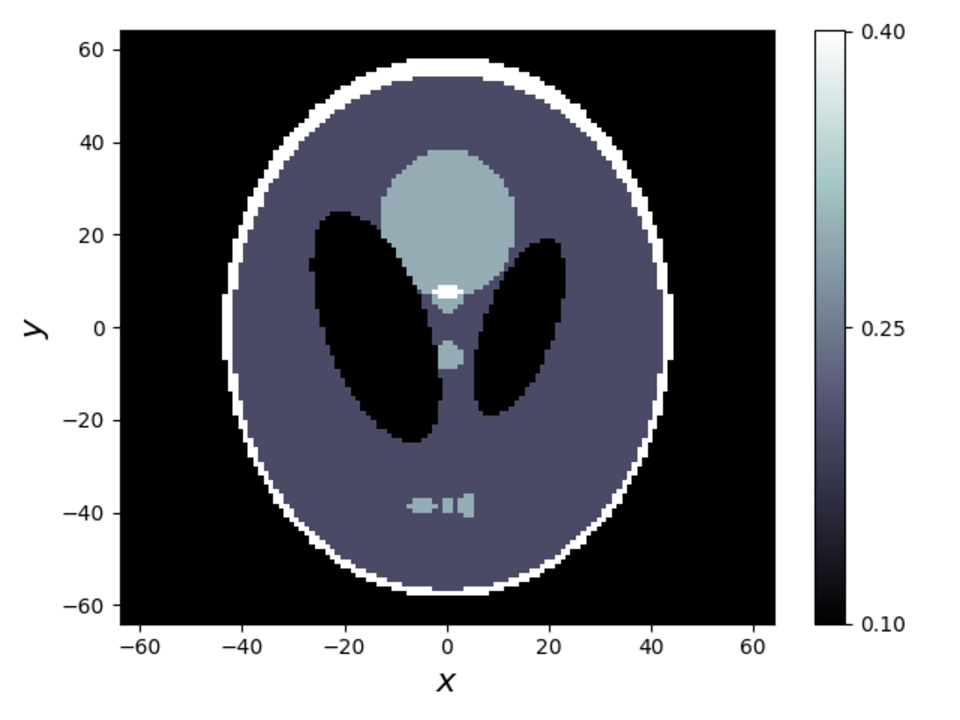
\includegraphics[width=0.49\columnwidth, trim={23mm 17mm 32mm 6mm}, clip]{true1} \hfill
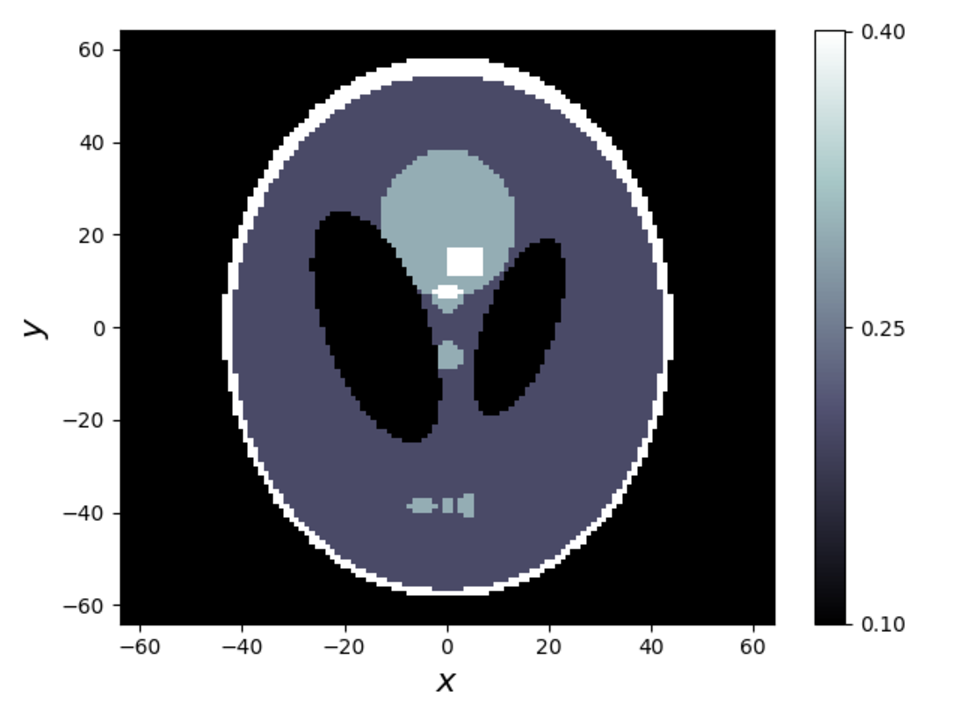
\includegraphics[width=0.49\columnwidth, trim={23mm 17mm 32mm 6mm}, clip]{true2} \\
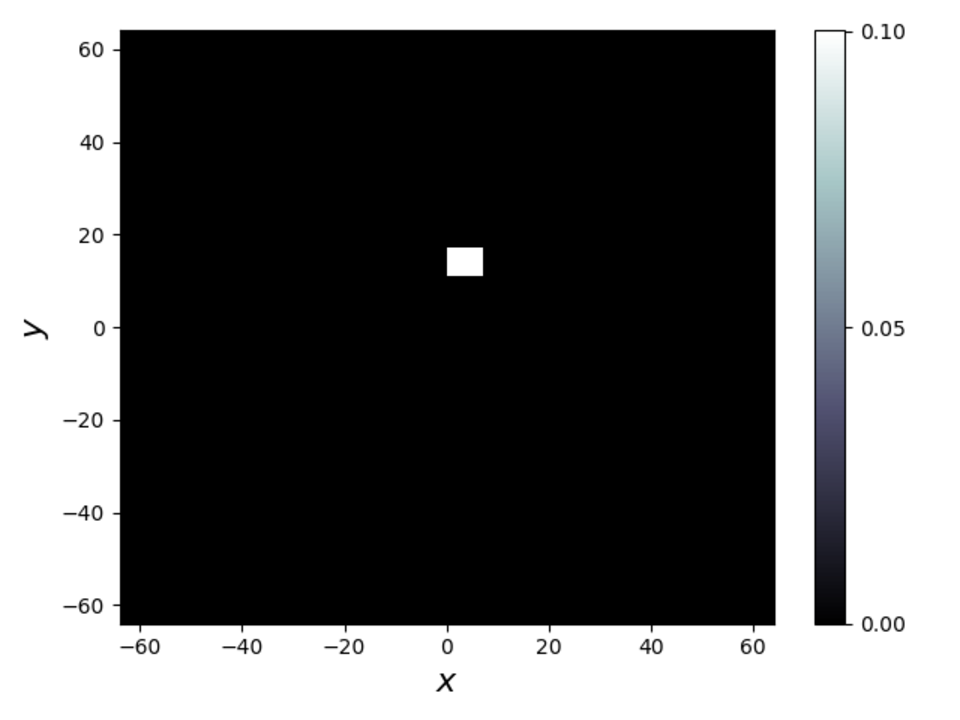
\includegraphics[width=0.49\columnwidth, trim={23mm 17mm 32mm 6mm}, clip]{difference_true} 
\end{column}
\hfill
\begin{column}{0.49\paperwidth}
\begin{overprint}
\onslide<2> % C=0.001
\centering
\captionfix{Reconstructions $C=0.001$}
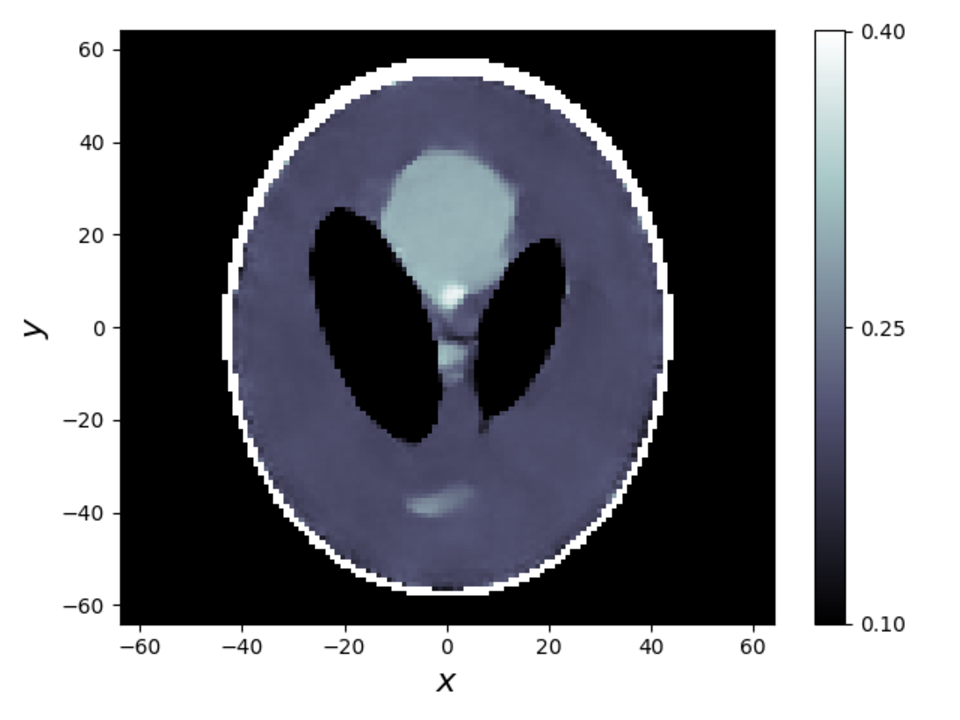
\includegraphics[width=0.49\columnwidth, trim={23mm 17mm 32mm 6mm}, clip]{recon1_0_001} \hfill
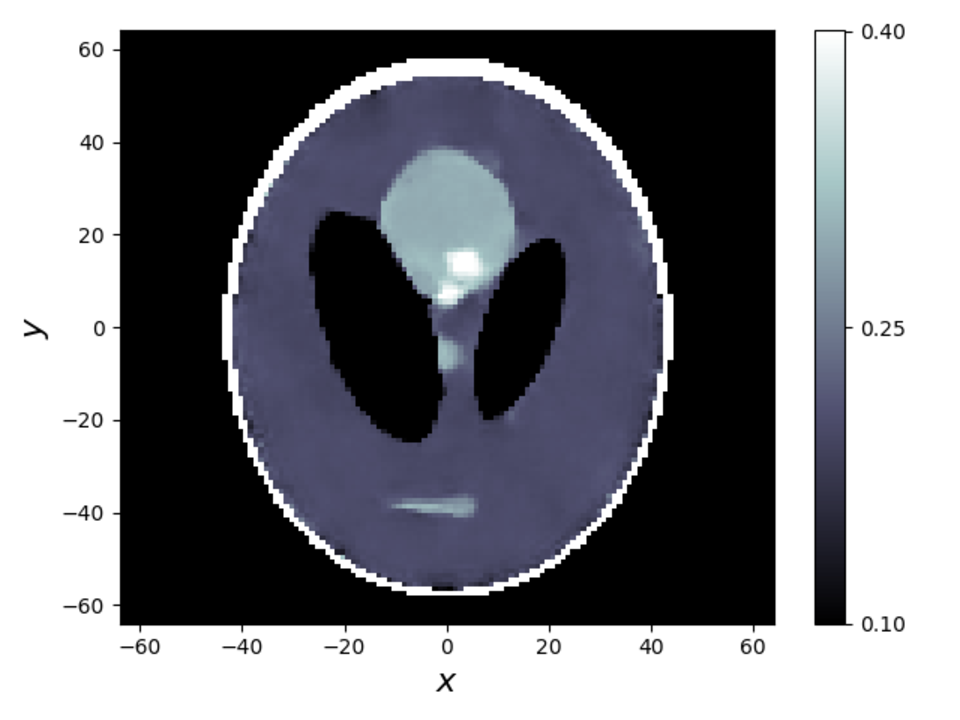
\includegraphics[width=0.49\columnwidth, trim={23mm 17mm 32mm 6mm}, clip]{recon2_0_001} \\
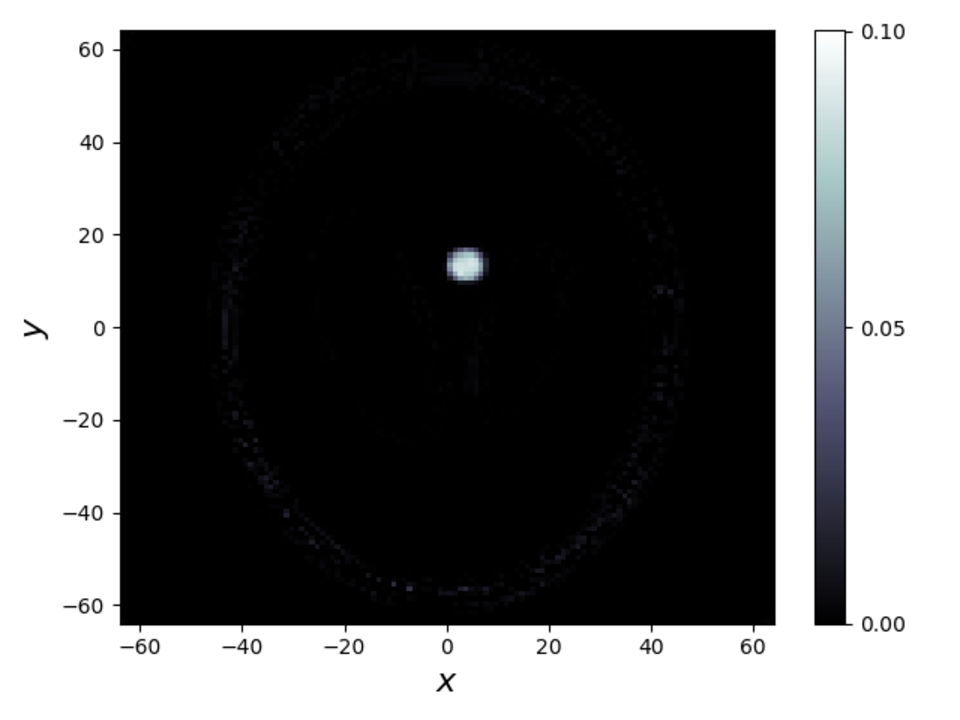
\includegraphics[width=0.49\columnwidth, trim={23mm 17mm 32mm 6mm}, clip]{difference_0_001} 
\onslide<3> % C=0.01
\centering
\captionfix{Reconstructions $C=0.010$}
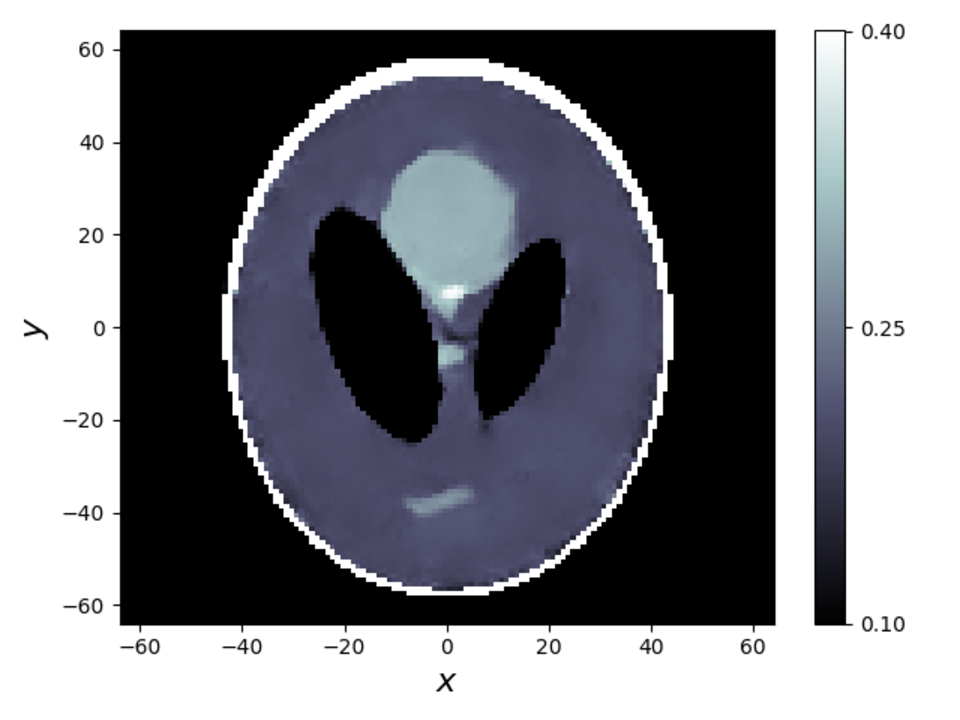
\includegraphics[width=0.49\columnwidth, trim={23mm 17mm 32mm 6mm}, clip]{recon1_0_010} \hfill
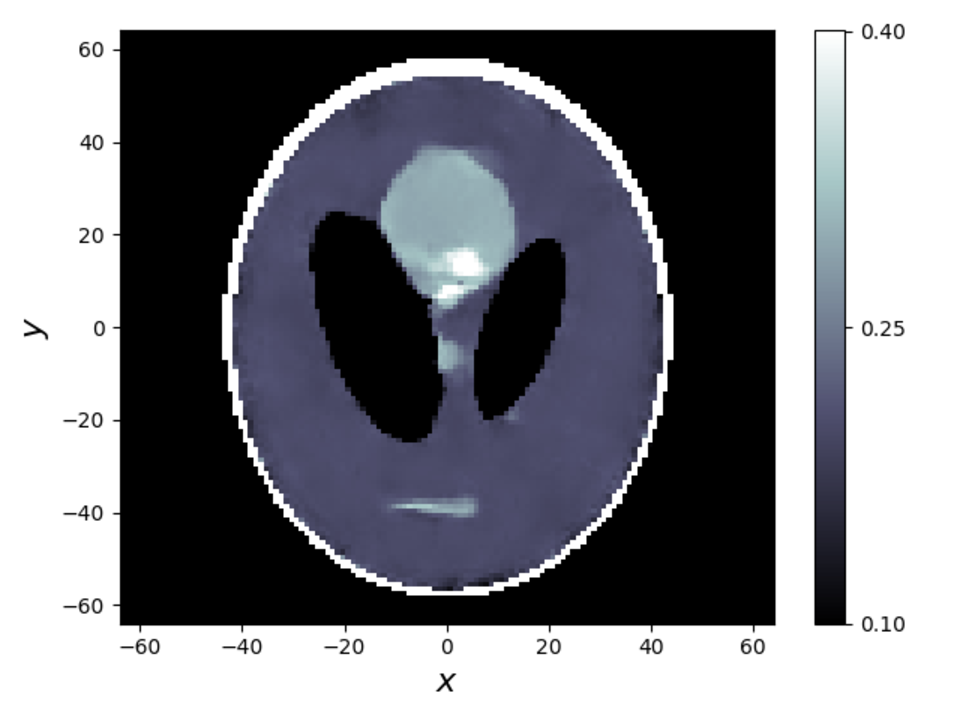
\includegraphics[width=0.49\columnwidth, trim={23mm 17mm 32mm 6mm}, clip]{recon2_0_010} \\
\includegraphics[width=0.49\columnwidth, trim={23mm 17mm 32mm 6mm}, clip]{difference_0_010} 
\onslide<4> % C=0.1
\centering
\captionfix{Reconstructions $C=0.10$}
\includegraphics[width=0.49\columnwidth, trim={23mm 17mm 32mm 6mm}, clip]{recon1_0_100} \hfill
\includegraphics[width=0.49\columnwidth, trim={23mm 17mm 32mm 6mm}, clip]{recon2_0_100} \\
\includegraphics[width=0.49\columnwidth, trim={23mm 17mm 32mm 6mm}, clip]{difference_0_100} 
\onslide<5> % C=1.0
\centering
\captionfix{Reconstructions $C=1.0$}
\includegraphics[width=0.49\columnwidth, trim={23mm 17mm 32mm 6mm}, clip]{recon1_1_0} \hfill
\includegraphics[width=0.49\columnwidth, trim={23mm 17mm 32mm 6mm}, clip]{recon2_1_0} \\
\includegraphics[width=0.49\columnwidth, trim={23mm 17mm 32mm 6mm}, clip]{difference_1_0} 
\onslide<6> % C=10.0
\centering
\captionfix{Reconstructions $C=10$}
\includegraphics[width=0.49\columnwidth, trim={23mm 17mm 32mm 6mm}, clip]{recon1_10_0} \hfill
\includegraphics[width=0.49\columnwidth, trim={23mm 17mm 32mm 6mm}, clip]{recon2_10_0} \\
\includegraphics[width=0.49\columnwidth, trim={23mm 17mm 32mm 6mm}, clip]{difference_10_0} 
\onslide<7> % C=100.0
\centering
\captionfix{Reconstructions $C=100$}
\includegraphics[width=0.49\columnwidth, trim={23mm 17mm 32mm 6mm}, clip]{recon1_100_0} \hfill
\includegraphics[width=0.49\columnwidth, trim={23mm 17mm 32mm 6mm}, clip]{recon2_100_0} \\
\includegraphics[width=0.49\columnwidth, trim={23mm 17mm 32mm 6mm}, clip]{difference_100_0} 
\onslide<8> % C=1000.0
\centering
\captionfix{Reconstructions $C=1000$}
\includegraphics[width=0.49\columnwidth, trim={23mm 17mm 32mm 6mm}, clip]{recon1_1000_0} \hfill
\includegraphics[width=0.49\columnwidth, trim={23mm 17mm 32mm 6mm}, clip]{recon2_1000_0} \\
\includegraphics[width=0.49\columnwidth, trim={23mm 17mm 32mm 6mm}, clip]{difference_1000_0} 
\onslide<9> % C=10 000.0
\centering
\captionfix{Reconstructions $C=10\,000$}
\includegraphics[width=0.49\columnwidth, trim={23mm 17mm 32mm 6mm}, clip]{recon1_10000_0} \hfill
\includegraphics[width=0.49\columnwidth, trim={23mm 17mm 32mm 6mm}, clip]{recon2_10000_0} \\
\includegraphics[width=0.49\columnwidth, trim={23mm 17mm 32mm 6mm}, clip]{difference_10000_0} 
\end{overprint}
\end{column}
\end{columns}
\end{frame}

% New frame
\begin{frame}{Joint reconstruction and classification of MNIST}
\begin{overprint}
\onslide<1>
\structure{Task based reconstruction problem:} Recover probabilities that MNIST image is a `0',`1', \ldots, `9'  from its  sinogram (tomographic data)
\[
\data = \ForwardOp(\signal) + \datanoise
\]
\begin{itemize}
\item Forward operator: Exponential of 2D ray transform (non-linear)
\item Geometry: Parallel beam, 25 lines/angle, 5 angles
\item Noise: Poisson noise corresponding to 60 photons measurement, i.e., 
  $\stdata \sim \frac{1}{60} \Poisson\bigl(60 \cdot \ForwardOp(\signaltrue) \bigr)$
\item Image: $28 \times 28$ pixel 
\item Training data: Triplets $(\signal_i,\data_i,\decision_i)$ where $\decision_i \in \{\text{`0'},\text{`1'}, \ldots, \text{`9'} \}$.
\end{itemize}
\onslide<2-4>
\begin{itemize}
\item \structure{Learned reconstruction $\model{\signalpara} \colon \DataSpace \to \RecSpace$}
\cite{Adler:2017aa}
\begin{itemize}
\item Learned gradient descent scheme
\item Distance: $\DistFunc{\RecSpace}$ is $L^2$-distance on $\RecSpace$
\end{itemize}
\visible<3->{
\item \structure{Learned task operator $\TaskOpLearned{\taskpara} \colon \RecSpace \to \DecisionSpace$ (classifier)}
\begin{itemize}
\item $\DecisionSpace =$ probability distributions over $\{\text{`0'},\text{`1'}, \ldots, \text{`9'} \}$
\item Given by `off the shelf' convolutional neural net classifier with 3 convolutional layers, each followed by $2 \times 2$ max pooling for segmentation
% The activation functions used were Relus. The layers had 32,64 and 128 channels respectively. I ended with one dense layer that transformed the output of the last convolutional layer to a logit layer of size 10, with the last activation function being a softmax.
\item Distance: $\DecisionDist$ is cross entropy
\end{itemize}
\visible<4->{
\item \structure{Task based reconstruction
$\TaskOpLearned{\taskpara} \circ \model{\signalpara} \colon \DataSpace \to \DecisionSpace$}
\begin{itemize}
\item Both networks pre-trained 
\begin{itemize}
\item Learned reconstruction pre-trained 
% using 500 steps with a batch size of 64 --> 64*500 = 32 000
\item Task operator (classifier) pre-trained until 97.5\% accuracy
% The amount of training steps used for that was around 1000 (again each training step on a batch of size 64)
\end{itemize}
\item Joint risk: Case with $C_1=C$ and $C_2=1-C$, i.e., 
\vskip-0.5\baselineskip
\[  \JointRisk(\signalpara,\taskpara) =
      \Expect\Bigl[  C \SignalDist(\signalpara) + (1-C) \, \DecisionDist(\taskpara) \Bigr].
\]      
\end{itemize}
}}
\end{itemize}
\end{overprint}
\end{frame}

% New frame
\begin{frame}{Joint reconstruction and classification of MNIST}

{\small
\begin{center}  
\begin{tabular}{l r r l}
  \toprule 
    Method & $L^2$-loss & CE-loss & Accuracy \\
  \otoprule  
  Case 1 & 10.3 & 0.41 & 93.35\% \\
  Case 2 & 14.7 & 0.13 & 96.00\% \\
  Case 3 & 19.6 & 0.40 & 90.95\% \\
  \alert<2>{Case 4} & \alert<2>{21.5} & \alert<2>{0.11} & \alert<2>{96.60\%} \\
  Clean data &  &  & 97.5\% \\
  \bottomrule
\end{tabular} 
\end{center}  
}
\begin{overprint}
\onslide<1>
\begin{itemize}
\item \structure{Case 1 -- Sequential pipeline}
\begin{itemize}
\item Reconstruction operator $\model{\signalpara}$ pre-trained with $L^2$-loss 
\item Classifier $\TaskOpLearned{\taskpara}$ pre-trained with cross-entropy loss
\end{itemize}
\item \structure{Case 2 -- Joint pipeline (partial joint training with $C=0$)}
\begin{itemize}
\item Reconstruction operator $\model{\signalpara}$ pre-trained with $L^2$-loss 
\item Classifier $\TaskOpLearned{\taskpara}$ trained with cross-entropy loss
\end{itemize}
\end{itemize}
\onslide<2>
\begin{itemize}
\item \structure{Case 3 -- Joint pipeline (partial joint training with $C=0$)}
\begin{itemize}
\item Reconstruction operator $\model{\signalpara}$ trained with cross-entropy loss
\item Classifier $\TaskOpLearned{\taskpara}$ pre-trained with cross-entropy loss
\end{itemize}
\item \structure{Case 4 -- Joint pipeline (with $C=0$)}
\begin{itemize}
\item $\model{\signalpara}$ and $\TaskOpLearned{\taskpara}$ both trained with cross-entropy loss.
\end{itemize}
\end{itemize}
\end{overprint}
\end{frame}


\begin{frame}[plain] %%%%% Joint reco + class of "4"
\begin{columns}[T]
\begin{column}{0.4\textwidth}
\begin{overprint}
\onslide<1-4> %% FBP
  \captionfix{FBP} 
  \centering
  \includegraphics[height=0.7\textheight,trim={9.75mm 49mm 3.5mm 3.2mm}, clip]{JointlyTrained_FBP_2} 
  \par\medskip
  \visible<2-4>{
    {\small
    \begin{tabular}{c r c r}
    \toprule 
      Class & Prob & Class & Prob \\
    \otoprule  
    `0' & 0.00\%  & `5' & 0.01\% \\
    `1' & 0.00\%  & `6' & 0.00\% \\
    `2' & 0.00\%  & `7' & 0.00\% \\
    `3' & 0.00\%  & \alert{`8'} & \alert{99.99\%} \\
    `4' & 0.00\%  & `9' & 0.00\% \\
    \bottomrule
    \end{tabular}}
  }
\onslide<5> %% Phantom
  \captionfix{Phantom} 
  \includegraphics[height=0.7\textheight,trim={9.75mm 49mm 3.5mm 3.2mm}, clip]{JointlyTrained_True_2}
  \par\bigskip
  \structure{True class:} `4'
\end{overprint}
\end{column}
\hfill
\begin{column}{0.4\textwidth}
\begin{overprint}
\onslide<3-5> %% Task based reco
  \captionfix{Task reco.: image} 
  \centering
  \visible<4-5>{
  \includegraphics[height=0.7\textheight,trim={9.75mm 49mm 3.5mm 3.2mm}, clip]{JointlyTrained_Reconstruction_2} 
  }
  \par\medskip
    {\small
    \begin{tabular}{c r c r}
    \toprule 
      Class & Prob & Class & Prob \\
    \otoprule  
    `0' & 0.00\%  & `5' & 0.00\% \\
    `1' & 0.00\%  & `6' & 0.00\% \\
    `2' & 0.00\%  & `7' & 0.00\% \\
    `3' & 0.00\%  & `8' & 0.00\% \\
    \alert{`4'} & \alert{99.70\%}  & `9' & 0.30\% \\
    \bottomrule
  \end{tabular}}
\end{overprint}
\end{column}
\end{columns}
\end{frame}

\begin{frame}[plain] %%%%% Joint reco + class of "4"
\begin{columns}[T]
\begin{column}{0.4\textwidth}
\begin{overprint}
\onslide<1-4> %% FBP
  \captionfix{FBP} 
  \centering
  \includegraphics[height=0.7\textheight,trim={9.75mm 49mm 3.5mm 3.2mm}, clip]{JointlyTrained_FBP_3} 
  \par\medskip
  \visible<2-4>{
    {\small
    \begin{tabular}{c r c r}
    \toprule 
      Class & Prob & Class & Prob \\
    \otoprule  
    `0' & 0.00\%  & `5' & 0.01\% \\
    `1' & 0.00\%  & `6' & 0.00\% \\
    `2' & 0.00\%  & `7' & 31.07\% \\
    `3' & 0.00\%  & `8' & 0.00\% \\
    \alert{`4'} & \alert{68.93\%}  & `9' & 0.00\% \\
    \bottomrule
    \end{tabular}}
  }
\onslide<5> %% Phantom
  \captionfix{Phantom} 
  \includegraphics[height=0.7\textheight,trim={9.75mm 49mm 3.5mm 3.2mm}, clip]{JointlyTrained_True_3}
  \par\bigskip
  \structure{True class:} `4'
\end{overprint}
\end{column}
\hfill
\begin{column}{0.4\textwidth}
\begin{overprint}
\onslide<3-5> %% Task based reco
  \captionfix{Task reco.: image} 
  \centering
  \visible<4-5>{
  \includegraphics[height=0.7\textheight,trim={9.75mm 49mm 3.5mm 3.2mm}, clip]{JointlyTrained_Reconstruction_3} 
  }
  \par\medskip
    {\small
    \begin{tabular}{c r c r}
    \toprule 
      Class & Prob & Class & Prob \\
    \otoprule  
    `0' & 0.00\%  & `5' & 0.00\% \\
    `1' & 0.00\%  & `6' & 0.00\% \\
    `2' & 0.00\%  & `7' & 0.00\% \\
    `3' & 0.00\%  & `8' & 0.00\% \\
    \alert{`4'} & \alert{99.97\%}  & `9' & 0.03\% \\
    \bottomrule
  \end{tabular}}
\end{overprint}
\end{column}
\end{columns}
\end{frame}

% Frame
\begin{frame}[plain] %%%%% Summary
\begin{columns}[T]
\begin{column}{0.24\textwidth}
\centering
\begin{overprint}
\onslide<1>
  \includegraphics[height=0.5\textheight,trim={9.75mm 49mm 3.5mm 3.2mm}, clip]{JointlyTrained_FBP_0} \\
  \includegraphics[height=0.5\textheight,trim={9.75mm 49mm 3.5mm 3.2mm}, clip]{JointlyTrained_FBP_1}
\onslide<2->
  \includegraphics[height=0.5\textheight,trim={9.75mm 49mm 3.5mm 3.2mm}, clip]{JointlyTrained_Reconstruction_0} \\
  \includegraphics[height=0.5\textheight,trim={9.75mm 49mm 3.5mm 3.2mm}, clip]{JointlyTrained_Reconstruction_1}
\end{overprint}
\end{column}
\begin{column}{0.24\textwidth}
\visible<3->{
  \includegraphics[height=0.5\textheight,trim={9.75mm 49mm 3.5mm 3.2mm}, clip]{JointlyTrained_True_0} \\
  \includegraphics[height=0.5\textheight,trim={9.75mm 49mm 3.5mm 3.2mm}, clip]{JointlyTrained_True_1}
}  
\end{column}
\quad
\begin{column}{0.24\textwidth}
\centering
\begin{overprint}
\onslide<1>
  \includegraphics[height=0.5\textheight,trim={9.75mm 49mm 3.5mm 3.2mm}, clip]{JointlyTrained_FBP_2} \\
  \includegraphics[height=0.5\textheight,trim={9.75mm 49mm 3.5mm 3.2mm}, clip]{JointlyTrained_FBP_3}
\onslide<2->
  \includegraphics[height=0.5\textheight,trim={9.75mm 49mm 3.5mm 3.2mm}, clip]{JointlyTrained_Reconstruction_2} \\
  \includegraphics[height=0.5\textheight,trim={9.75mm 49mm 3.5mm 3.2mm}, clip]{JointlyTrained_Reconstruction_3}
\end{overprint}
\end{column}
\begin{column}{0.24\textwidth}
\visible<3->{
  \includegraphics[height=0.5\textheight,trim={9.75mm 49mm 3.5mm 3.2mm}, clip]{JointlyTrained_True_2} \\
  \includegraphics[height=0.5\textheight,trim={9.75mm 49mm 3.5mm 3.2mm}, clip]{JointlyTrained_True_3}
}
\end{column}
\end{columns}
\end{frame}

% New frame
\begin{frame}{Advertisement}{PhD position in Deep Dictionary Learning at KTH Royal Institute of Technology}
\begin{center}
  \includegraphics[height=0.5\textheight]{Stockholm}
\end{center}
\begin{itemize}
\item Development of theory and algorithms that \alert{combine} methods from machine learning with sparse signal processing for 
joint dictionary design and image reconstruction for clinical 3D axial/helical CT and spectral CT.
\item Joint project with Philips Healthcare, Hamburg.
\item Deadline: 30 April 2018
\item Link: \href{https://kth.mynetworkglobal.com/en/what:job/jobID:203304/where:4/}{https://kth.mynetworkglobal.com/en/what:job/jobID:203304/where:4/}
\end{itemize}
\end{frame}


% New frame
\begin{frame}[plain]
\centering
$\,$\vfill
{\Large \structure{Thank you for your attention!}}
\vfill$\,$
\end{frame}

% New frame
\begin{frame}[t, allowframebreaks]
\frametitle{References}
\bibliographystyle{apacite}
\bibliography{refLect3}
\end{frame}

\end{document}



